% Impostazioni principali
\documentclass[t, compress, mathserif]{beamer}



%         ----------------------------------------------         %
%        /                                              \        %
%--------               START PREAMBLE                   --------%
%        \                                              /        %
%         ----------------------------------------------         %

% Titolo che appare nella prima slide del documento
\newcommand{\titolo}{Examples and exercises - Basic Statistics}
\newcommand{\sottotitolo}{}

% Titolo che appare nella barra in basso di ogni slide, al centro
% Sono due variabili:
% * una puo' essere utilizzata per l'intero corso. Se impostata nel preambolo sovrascrive quella di seguito.
% * l'altra puo' identificare ciascun documento
\newcommand{\titolocompleto}{Statistics course - }
\newcommand{\titoloshort}{\titolo}

% Numero di capitolo o altro nome che appare in basso di ogni slide, vicino al numero di pagina
\newcommand{\numerocapitolo}{}

% Include il documento che contiene il preambolo
\input{../includeTex/preamble.tex}

% Numero di slide per pagina
\usepackage{pgfpages}
\pgfpagesuselayout{2 on 1}[a4paper, border shrink = 3mm]
% \pgfpagesuselayout{4 on 1}[a4paper, border shrink = 3mm, landscape]


%         ----------------------------------------------         %
%        /                                              \        %
%--------               START DOCUMENT                   --------%
%        \                                              /        %
%         ----------------------------------------------         %

\begin{document}

% Pagina del titolo
\frame{\titlepage}

% Indice
% \begin{frame}
% 	 \tableofcontents
% \end{frame}

% Documento
% I soli contenuti del documento sono in un file esterno. Questo semplifica enormemente le cose qualora si volessero creare dei manuali (singoli documenti) a partire da diversi documenti.
\livelloA{Elementary Statistics}

\livelloB{Comparison of the postcards sales in two countries}

\begin{frame} 
\begin{description}
\item[Data:] cardsales.txt\\
Postcard sales data in the countries of New York and Florida day by day, from 1 January to 31 March.
\item[Aims:] \begin{itemize}
\item 
Let us numerically and graphically evaluate the distribution of the number of postcards sold in the two countries.
\begin{itemize}
\item[-] Which country has sold the most?
\item[-] Which country has more variability? 
\item[-] Are there anomalies?
\end{itemize}
\item Let us graphically check if the number of postcards sold daily in the two countries ``is associated '' somehow.
\end{itemize}

\end{description}
 
\end{frame}

%%%%%%%%%%%%%%%%%%%%%%%%%%%%%%%%%%%%%%%%%%%%%%%%%%%%%%%%%%%%%%%
\begin{frame}
Computation of descriptive statistics and B-W graphic:\\
	\vspace{.3cm}
	\begin{footnotesize}
	\begin{tabular}{|l|rrrrrrr|}
	\hline
	& \textbf{Min}. & 1\textbf{st.Qu}. & \textbf{Median} & \textbf{Mean} & \textbf{3rd.Qu.} & \textbf{Max.} & \textbf{Sd}\\
	\hline
	\textbf{FL.Sales (N=91)} & 1420 & 1484 & 1514 & 1514 & 1544 & 1640 & 46.52 \\
	\textbf{NY.Sales (N=91)} & 0 & 1654 & 1687 & 1671 & 1720 & 1813 & 183.65 \\
	\hline	
	\end{tabular}
	\end{footnotesize}
	\begin{center}
		\includegraphics[width=6cm]{14_1.png}
	\end{center}
\end{frame}


%%%%%%%%%%%%%%%%%%%%%%%%%%%%%%%%%%%%%%%%%%%%%%%%%%%%%%%%%%%%%%%
\begin{frame}
\begin{itemize}
 \item Both the mean and the standard deviation of the sold in New York are greater than the respective statistics of the sold in Florida.
 \item It is necessary to note that the sold in New York has at least one day with 0 cards.
 \item Analysing the data, It is possible to understand that the day 20 of January, 0 postcards have been sold in New York because of a strike.
 \item That value will be removed to analyse again the data, in order to understand if the differences are still as relevant. 
\end{itemize}

\end{frame}

%%%%%%%%%%%%%%%%%%%%%%%%%%%%%%%%%%%%%%%%%%%%%%%%%%%%%%%%%%%%%%%
\begin{frame}
Computation of descriptive statistics and B-W graphic: (0 of NY deleted):\\
	\vspace{.3cm}
	\begin{footnotesize}
	\begin{tabular}{|l|rrrrrrr|}
	\hline
	& \textbf{Min.} & \textbf{1st.Qu.} & \textbf{Median} & \textbf{Mean} & \textbf{3rd.Qu.} & \textbf{Max.} & \textbf{Sd}\\
	\hline
	\textbf{FL.Sales (N=91)} & 1420 & 1484 & 1514 & 1514 & 1544 & 1640  & 46.52 \\
	\textbf{NY.Sales (N=90)} & 1587 & 1656 & 1687 & 1690 & 1721 & 1813 & 48.65 \\
	\hline	
	\end{tabular}
	\end{footnotesize}
	\begin{center}
		\includegraphics[width=6cm]{14_2.png}
	\end{center}
\end{frame}

%%%%%%%%%%%%%%%%%%%%%%%%%%%%%%%%%%%%%%%%%%%%%%%%%%%%%%%%%%%%%%%
\begin{frame}
\begin{itemize}
 \item The elimination of the 0 value has changed much the values of the statistics for only New York.
 \item Mean and median of the number of postcards sold daily are greater for New York.
 \item Indeed, New York has a number of postcards sold daily almost always higher than the Florida.
 \item The dispersion in the two countries is very similar.
 \item The distribution of the number of postcards sold, in general, seems to differ only for location.
\end{itemize}

\end{frame}

%%%%%%%%%%%%%%%%%%%%%%%%%%%%%%%%%%%%%%%%%%%%%%%%%%%%%%%%%%%%%%%
\begin{frame}
	\begin{center}
		\includegraphics[width=7cm]{14_3.png}
	\end{center}
\begin{footnotesize}There are no relationship between the postcards sold in New York and in Florida.
\end{footnotesize}\end{frame}

%%%%%%%%%%%%%%%%%%%%%%%%%%%%%%%%%%%%%%%%%%%%%%%%%%%%%%%%%%%%%%%
\begin{frame} 
	\begin{center}
		\includegraphics[width=7cm]{14_4.png}
	\end{center}
\begin{footnotesize}There are no relationship between the postcards sold in New York and in Florida.
\end{footnotesize}\end{frame}

%%%%%%%%%%%%%%%%%%%%%%%%%%%%%%%%%%%%%%%%%%%%%%%%%%%%%%%%%%%%%%%
\livelloB{Comparison between an adjusted and a non adjusted productive process}

%%%%%%%%%%%%%%%%%%%%%%%%%%%%%%%%%%%%%%%%%%%%%%%%%%%%%%%%%%%%%%%
\begin{frame} 
\begin{description}
	\item[Data:] adjust.txt\\
	Monitoring data of two production processes equal but one constantly monitored, while the other not.
	\item[Aims:] \begin{itemize}
				\item Let us numerically and graphically evaluate if It is better to monitor the processes knowing that, for the parameter analysed, the technically acceptable values must fall between 1,485 and 1,515, with central value in 1.5. 
				\begin{itemize}
					\item[-] Which are the main statistics of the two processes?
					\item[-] Which process is better? 
					\item[-] Why? 
					\item[-] What is the difference in performance of the two processes?
				\end{itemize}
				\item Let us do numerical and graphical analysis.
	                  \end{itemize}
\end{description}
\end{frame}

%%%%%%%%%%%%%%%%%%%%%%%%%%%%%%%%%%%%%%%%%%%%%%%%%%%%%%%%%%%%%%%
\begin{frame}
Computation of descriptive statistics and B-W graphic:
	\vspace{.3cm}
	\begin{footnotesize}
	\begin{tabular}{|l|rrrrrrr|}
	\hline
	& \textbf{Min}. & 1\textbf{st.Qu}. & \textbf{Median} & \textbf{Mean} & \textbf{3rd.Qu.} & \textbf{Max.} & \textbf{Sd}\\
	\hline
	\textbf{Adjust (N=50)} & 1.475 & 1.492 & 1.499 & 1.500 & 1.509 & 1.525 & 0.0128\\
	\textbf{NoAdjust (N=50)} & 1.480 & 1.495  & 1.499 & 1.498 & 1.504 & 1.509 & 0.0070\\
	\hline	
	\end{tabular}
	\end{footnotesize}
	\begin{center}
		\includegraphics[width=6cm]{14_5.png}
	\end{center}
\end{frame}

%%%%%%%%%%%%%%%%%%%%%%%%%%%%%%%%%%%%%%%%%%%%%%%%%%%%%%%%%%%%%%%
\begin{frame}
	\begin{center}
		\includegraphics[width=7cm]{14_6.png}
	\end{center}
  \begin{center}  
\begin{footnotesize}Histograms illustrating the distribution of the data for the two processes.
\end{footnotesize}
  \end{center}
\end{frame}

%%%%%%%%%%%%%%%%%%%%%%%%%%%%%%%%%%%%%%%%%%%%%%%%%%%%%%%%%%%%%%%
\begin{frame}
  \begin{itemize}
    \item Data of both processes are centered around the central value of  technical acceptability.
    \item Both processes have a symmetrical distribution around the center. 
    \item The adjusted process seems to have a greater variability than the non adjusted process.
  \end{itemize}
\end{frame}

%%%%%%%%%%%%%%%%%%%%%%%%%%%%%%%%%%%%%%%%%%%%%%%%%%%%%%%%%%%%%%%
\begin{frame}
	\begin{center}
		\includegraphics[width=7cm]{14_7.png}
	\end{center}
\begin{center}  
\begin{footnotesize} The adjusted process is more variable. The non adjusted process seems to ``go to drift'' downward in the last measurements.
\end{footnotesize}
  \end{center}
\end{frame}

%%%%%%%%%%%%%%%%%%%%%%%%%%%%%%%%%%%%%%%%%%%%%%%%%%%%%%%%%%%%%%%
\begin{frame}
  \begin{itemize}
    \item If you try to see how many times you have had out of specification values for each of the two processes, you obtain the following tables:
  \end{itemize}
  \begin{center}
    \begin{tabular}{|l|rr|c|l|rr|}
      \hline	
      \textbf{AdjustIn} & \textbf{No} & \textbf{S\`i} & & \textbf{NoAdjustIn} &  \textbf{No} & \textbf{S\`i} \\
      \hline
      \textbf{Counts} & 12 & 38 & & \textbf{Counts} & 3 & 47 \\
      \textbf{\%} & 24\% & 76\% & & \textbf{\%} & 6\% & 94\% \\
      \hline
    \end{tabular} 
  \end{center}
  \begin{itemize}
    \item It is evident how the non continuous adjusted processes generates a better final product, because It is more within specifications.
    \item Probably the continuous intervention of the operator in turn induces constant shifts in the average value of the process, increasing the variability to the process itself.
    \item The adjusted process produces significantly fewer pieces out of specification, as shown later (see the part relative to hypothesis testing).
  \end{itemize}
\end{frame}

%%%%%%%%%%%%%%%%%%%%%%%%%%%%%%%%%%%%%%%%%%%%%%%%%%%%%%%%%%%%%%%
\livelloB{Bond Strength Analysis}

%%%%%%%%%%%%%%%%%%%%%%%%%%%%%%%%%%%%%%%%%%%%%%%%%%%%%%%%%%%%%%%
\begin{frame} 
 
\begin{description}
	\item[Data:] bondstrength.txt\\
  Comparison data of the bond strenght of different formualtions of glues over time.
	\item[Aims:] \begin{itemize}
				\item Data of the strength necessary to separate two bonded surfaces with 6 different formulations of adhesive at a distance of 3, 6, 9 months is detected. 
				\begin{itemize}
					\item[-] Let us compare the holding of the 6 formulations.
					\item[-] Are there different variabilities in the 6 formulations?
					\item[-] Check if the holding decreases over time.
					\item[-] What are the formulations that satify the minimum requirement of holding 50 kg?
				\end{itemize}
				\item Let us do numerical and graphical analysis.
	                  \end{itemize}
\end{description}
 
\end{frame}

%%%%%%%%%%%%%%%%%%%%%%%%%%%%%%%%%%%%%%%%%%%%%%%%%%%%%%%%%%%%%%%
\begin{frame}
Computation of descriptive statistics and B-W graphic:\\
	\vspace{.3cm}
	\begin{footnotesize}
	\begin{tabular}{|l|rrrrrrr|}
	\hline
	& \textbf{Min}. & 1\textbf{st.Qu}. & \textbf{Median} & \textbf{Mean} & \textbf{3rd.Qu.} & \textbf{Max.} & \textbf{Sd}\\
	\hline
	\textbf{1+1 A} (N=72)& 43.00& 50.20& 53.50& 53.62& 57.50& 62.40& 4.34\\
	\textbf{1+1 B} (N=72)& 56.20& 64.00& 67.55& 67.23& 70.95& 74.60& 3.98\\
	\textbf{1+1 W} (N=72)& 47.90& 53.15& 54.80& 55.07& 56.97& 64.70& 3.19\\
	\textbf{2+2 B} (N=72)& 56.50& 63.82& 66.60& 66.27& 68.48& 77.70& 4.34\\
	\textbf{SS}    (N=72)& 25.90& 35.18& 40.55& 39.47& 44.05& 58.00& 6.24\\
	\textbf{XF}    (N=72)& 25.60& 33.65& 37.45& 37.83& 41.78& 56.00& 6.55\\
	\hline	
	\end{tabular}
	\end{footnotesize}
	\begin{center}
		\includegraphics[width=6cm]{14_8.png}
	\end{center}
\end{frame}

%%%%%%%%%%%%%%%%%%%%%%%%%%%%%%%%%%%%%%%%%%%%%%%%%%%%%%%%%%%%%%%
\begin{frame}
\begin{itemize}
 \item It seems that the formulations with better holding are those characterized by the code \textbf{B}.
 \item The formulation with greater mean and median holding is \textbf{1+1 B}.
 \item The formualtions with lesser holding are \textbf{SS} and \textbf{XF}. These formulations have also a greater variability.
 \item The formulations \textbf{A} and \textbf{W} seem to have a non evedently higher variability than  \textbf{B}.
 \item The formulation \textbf{1+1 W} is the one with lesser variability.
 \item All the formulations present a distribution of the strength of separation approximately symmetrical.  
 \item The formulations that certainly satisfy the 50kg criterion, at least for the observed data, are \textbf{1+1 B} and  \textbf{2+2 B}. 
 \end{itemize}

\end{frame}

%%%%%%%%%%%%%%%%%%%%%%%%%%%%%%%%%%%%%%%%%%%%%%%%%%%%%%%%%%%%%%%
\begin{frame}
	\vspace{.3cm}
	\begin{center}
		\includegraphics[width=9cm]{14_9.png}
	\end{center}
    \begin{center}
\begin{footnotesize}
 Description of the separation strength of the different formulations of glue varying the months (reference line: 50Kg). 
\end{footnotesize}
  \end{center}
\end{frame}

%%%%%%%%%%%%%%%%%%%%%%%%%%%%%%%%%%%%%%%%%%%%%%%%%%%%%%%%%%%%%%%
\begin{frame}
\begin{itemize}
 \item The impression given by the analysis of the formulations are confirmed.
 \item Over time, the bond strength decreases for the worst formulations. 
 \item The formulations with greater holding highligth a certain stability over time.
 \end{itemize}
\end{frame}



\livelloA{Correlation}

\livelloB{Mean diameter of caps produced by a forging machine}

\begin{frame} 
 
\begin{description}
	\item[Data:] bottlecap.txt\\
	\item[Aims:] Data of the mean diameter of the caps produced by a forging machine (let us see the following picture).
 Let us check if the caps diameter measures are correlated, so that It is possible to non measure all tha caps produced by the same machine in quality control phase.
				\begin{itemize}\begin{footnotesize}
					\item[-] Let us compute the main descriptive statistics for each cavity. 
					\item[-] Let us compute the correlations between the measures of cavities.
					\item[-] Let us graphically represent the diameter values between the pairs of cavities.
					\item[-] Is there very related cavities, enough to be ``replaceable'' in the measurements?  
				\end{footnotesize}\end{itemize}

\end{description}
 
\end{frame}

%%%%%%%%%%%%%%%%%%%%%%%%%%%%%%%%%%%%%%%%%%%%%%%%%%%%%%%%%%%%%%%
\begin{frame}
Scheme of the mould of caps:
\vspace{.3cm}
	\begin{center}
		\includegraphics[width=6cm]{14_20.png}
	\end{center}
\end{frame}

%%%%%%%%%%%%%%%%%%%%%%%%%%%%%%%%%%%%%%%%%%%%%%%%%%%%%%%%%%%%%%%
\begin{frame}
Correlation matrix:\\
\vspace{.3cm}
\begin{tiny}
\begin{tabular}{l|rrrrrrrr}
         & Cavity.1 & Cavity.2 & Cavity.3 & Cavity.4 & Cavity.5 & Cavity.6 & Cavity.7 & Cavity.8\\
\hline
Cavity.1    & 1.000    & 0.858    & 0.650   & 0.459    & 0.193   & -0.115   & -0.037    & 0.343\\
Cavity.2    & 0.858    & 1.000    & 0.869    & 0.698    & 0.490    & 0.337   & 0.344    & 0.685\\
Cavity.3    & 0.650    & 0.869    & 1.000    & 0.604    & 0.471    & 0.401    & 0.399    & 0.601\\
Cavity.4    & 0.459    & 0.698    & 0.604    & 1.000    & 0.778    & 0.583    & 0.327    & 0.629\\
Cavity.5    & 0.193    & 0.490    & 0.471    & 0.778    & 1.000    & 0.627    & 0.417    & 0.627\\
Cavity.6   & -0.115    & 0.337    & 0.401    & 0.583    & 0.627    & 1.000    & 0.847    & 0.747\\
Cavity.7   & -0.037    & 0.344    & 0.399    & 0.327    & 0.417    & 0.847    & 1.000    & 0.542\\
Cavity.8    & 0.343    & 0.685    & 0.601    & 0.629    & 0.627    & 0.747    & 0.542    & 1.000\\
\end{tabular} 
\end{tiny}
\end{frame}

%%%%%%%%%%%%%%%%%%%%%%%%%%%%%%%%%%%%%%%%%%%%%%%%%%%%%%%%%%%%%%%
\begin{frame}
Scatterplot matrix of the relations between measures:
\vspace{.3cm}
	\begin{center}
		\includegraphics[width=7.5cm]{14_21.png}
	\end{center}
\end{frame}

%%%%%%%%%%%%%%%%%%%%%%%%%%%%%%%%%%%%%%%%%%%%%%%%%%%%%%%%%%%%%%%
\begin{frame}
\begin{itemize}
 \item Many of the measures have a high correlation value ($>.7$).
 \item In particular, the measures of Cavity.1 and Cavity.2, Cavity.2 and Cavity.3, Cavity.6 and Cavity.7 have a correlation value greater than .845. 
 \item Therefore the value of Cavity.2 instead of Cavity.1, or instead of Cavity.3 could be used.
 \item \textbf{Interesting note}: The correlations are not transitive: the correlation between Cavity.1 and Cavity.3 is .65, the correlation between Cavity.3 and Cavity.6 is .401; the correlation between Cavity.1 and Cavity.6 is negative! 
 \end{itemize}

\end{frame}


%%%%%%%%%%%%%%%%%%%%%%%%%%%%%%%%%%%%%%%%%%%%%%%%%%%%%%%%%%%%%%%
\livelloB{pH measure tools}
\begin{frame} 
 
\begin{description}
	\item[Data:] labtest.txt\\ 
	Comparison between the pH measure tools on the same samples of material.
	\item[Aims:] \begin{small}\begin{itemize}
				\item Let us check if the two tools (in lab and ``on the field'') give correlated values by measuring the same samples.
				\begin{itemize}
					\item[-] Let us compute the correlations between the measurements of the two equipments.
					\item[-] Let us graphically represent the diameter values between the pairs of measurements.
				\end{itemize}
	                  \end{itemize}
\end{small}
\end{description}
 
\end{frame}

%%%%%%%%%%%%%%%%%%%%%%%%%%%%%%%%%%%%%%%%%%%%%%%%%%%%%%%%%%%%%%%
\begin{frame}
Correlation matrix:\\
\vspace{.3cm}
\begin{footnotesize}
\begin{tabular}{l|rr}
 & Lab & Online\\
\hline
Lab & 1.000 & 0.959\\
Online & 0.959 & 1.000\\
\end{tabular} 
\end{footnotesize}

Scatterplot matrix of the relations between measures:
\vspace{.3cm}
	\begin{center}
		\includegraphics[width=5.5cm]{14_22.png}
	\end{center}
\end{frame}

%%%%%%%%%%%%%%%%%%%%%%%%%%%%%%%%%%%%%%%%%%%%%%%%%%%%%%%%%%%%%%%
\begin{frame}
Scatterplot della relazione con retta di regressione:\\
\vspace{.3cm}
	\begin{center}
		\includegraphics[width=6.5cm]{14_23.png}
	\end{center}
\end{frame}

%%%%%%%%%%%%%%%%%%%%%%%%%%%%%%%%%%%%%%%%%%%%%%%%%%%%%%%%%%%%%%%
\begin{frame}
\begin{itemize}
 \item The two measurements have a very high correlation value.  
 \item Considering the correlation, the two tools could be ``almost'' interchangeable. However, considering the previous analysis, which analyse the differences in pairs between the measured values, the on-line tool seems to produce values systematically different from the laboratory instrument.
 \end{itemize}

\end{frame}


\livelloA{Test Z and t}

\livelloB{Filling cereal boxes}

\begin{frame} 
  \begin{description}
    \item[Data:] cerealbx.txt\\ 
      Data on the filling of cereal boxes.
    \item[Aims: ]
      \begin{small}
        A process of filling cereal boxes needs that each box contains on average 365 grams of cereals. Let us check to if the current process actually follows this constraint.

        \begin{itemize}
          \item[-] Let us compute the descriptive statistics on data.
          \item[-] Let us graphically summarise data.
          \item[-] Let us try to check the hypothesis that the mean is 365 in the case that the standard deviation shall be 2.4.
          \item[-] Let us try to verify the same hypothesis assuming that the standard deviation is unknown. What are the differences in respect to the previous test? Why?
          \item[-] Let us compute the 95\%  confidence interval for the mean in both cases.
        \end{itemize}
      \end{small}
  \end{description}
\end{frame}

\begin{frame}
  Computation of descriptive statistics and B-W graphic:\\
  \vspace{.3cm}
  \begin{footnotesize}
    \begin{tabular}{|l|rrrrrrr|}
      \hline
      & \textbf{Min}. & 1\textbf{st.Qu}. & \textbf{Median} & \textbf{Mean} & \textbf{3rd.Qu.} & \textbf{Max.} & \textbf{Sd}\\
      \hline
      \textbf{BoxWeigh (N=6)} & 363.4 & 365.1 & 367.2 & 366.7 & 367.7 & 370.1 & 2.4029\\
      \hline	
    \end{tabular}
  \end{footnotesize}
  \begin{center}
    \includegraphics[width=6cm]{14_10.png}
  \end{center}
\end{frame}

\begin{frame}[fragile]
  Computation of Z test:
  \begin{verbatim}
Z = 1.7396, p-value = 0.08192
alternative hypothesis: true mean is not equal to 365
95 percent confidence interval:
 364.7841 368.6249
sample estimates:
mean of x: 366.7045
  \end{verbatim}
\end{frame}

\begin{frame}[fragile]
  Computation of t test:
  \begin{verbatim}
t = 1.7375, df = 5, p-value = 0.1428
alternative hypothesis: true mean is not equal to 365
95 percent confidence interval:
 364.1828 369.2262
sample estimates:
mean of x: 366.7045
  \end{verbatim}
\end{frame}

\begin{frame}
  \begin{itemize}
    \item According to tests Z there is no evidence that the current process does not respect the parameters expected.
    \item The t-test confirms this result.
    \item The two tests give a different value of p-value: in particular the p-value of Z  test is lower than that of the t test. This is due to the fact that the t test has a reference distribution ($t_{5}$) much more dispersed than the Z test ($N(0,1)$). As the value of Z test and of t test are nearly equal, the probability to obtain ``outer'' values to the value of the test will be higher for the  more dispersed distribution.
    \item As a consequence of this statement, also the confidence interval computed under the hypothesis of knowing the standard deviation value of data results to be more ``tight'' than that computed under the hypothesis of not knowing the standard deviation value. 
  \end{itemize}
\end{frame}

\livelloB{Check the milk quality}

\begin{frame} 
  \begin{description}
    \item[Data:] cheese.txt\\ 
      Data of the freezing temperature of the milk supply.
    \item[Aims:] \begin{small}A cheese factory receives milk from its suppliers. The owner suspects that milk received from one of the suppliers is ``watered down''. To check that, he collects milk samples and he checks the characteristics measuring the freezing temperature. If the milk is ``good'', It should freeze at a temperature on average not higher than -0.545$^o$C.\end{small}  
      \begin{itemize} \begin{small}
        \item[-] Let us compute the main descriptive statistics and let us graphically summarise data.
        \item[-] Let us try to check the if the average temperature is not higher than -0.545$^o$C against if It is.
        \item[-] Let us try to apply a two-sided test. What are the results? Why is there a difference?
        \item[-] Let us compute the 95\% confidence interval of the mean in both cases.
      \end{small}\end{itemize}
  \end{description}
\end{frame}

\begin{frame}
  Computation of descriptive statistics and B-W graphic:\\
  \vspace{.3cm}
  \begin{scriptsize}
    \begin{tabular}{|l|rrrrrrr|}
      \hline
      & \textbf{Min}. & 1\textbf{st.Qu}. & \textbf{Median} & \textbf{Mean} & \textbf{3rd.Qu.} & \textbf{Max.} & \textbf{Sd}\\
      \hline
      \textbf{FrzTemp(N=10)} & -0.5562 & -0.5427 & -0.5381 & -0.5394 & -0.5335 & -0.5311 & 0.0078\\
      \hline	
    \end{tabular}
  \end{scriptsize}
  \begin{center}
    \includegraphics[width=6cm]{14_11.png}
  \end{center}
\end{frame}

\begin{frame}[fragile]
  Computation of t test (unilateral hypothesis):
  \begin{verbatim}
t = 2.2835, df = 9, p-value = 0.02414
alternative hypothesis: true mean is greater than -0.545
95 percent confidence interval:
 -0.5438892        Inf
sample estimates:
mean of x: -0.5393685
  \end{verbatim}
\end{frame}

\begin{frame}[fragile]
  Computation of t test (bilateral hypothesis):
  \begin{verbatim}
t = 2.2835, df = 9, p-value = 0.04828
alternative hypothesis: true mean is not equal to -0.545
95 percent confidence interval:
 -0.5449473 -0.5337897
sample estimates:
mean of x: -0.5393685
  \end{verbatim}
\end{frame}

\begin{frame}
  \begin{itemize}
    \item The unilateral test rejects the hypothesis that the milk is not watered down.
    \vspace{0.75cm}
    \item Also the bilateral test rejects this hypothesis, but with a p-value very close to 0.05; so It obtains a ``borderline'' result.
    \vspace{0.75cm}
    \item The difference between the two tests is found only on the value of the p-value; all the others statistics (apart from the confidence intervals) are equal.
  \end{itemize}
\end{frame}

\livelloB{Ball bearings diameter}

\begin{frame} 
  \begin{description}
    \item[Data:] bearings.txt\\ 
      Data on the measurements of the ball bearings diameter.
    \item[Aims:]
      \begin{small}
        A mechanical firm produces ball bearings. From past experience, It is known that the standard deviation of the diameter measurements is about 0.004 cm. 10 bearings have been collected to check the hypothesis that the mean value is equal to 0.5 cm. 
        \begin{itemize}
          \item[-] Let us compute the main descriptive statistics and let us graphically summarise  the data.
          \item[-] Let us check the hypothesis that the mean diameter is 0.5 cm against the hypothesis that It is not using Z and t test.
          \item[-] Let us compute the 95\% confidence interval for the mean in both cases.
          \item[-] Let us check the hypothesis of normality of the data using Normal Probability Plot and A-D test. 
        \end{itemize}
      \end{small}
  \end{description}
\end{frame}

\begin{frame}
  Computation of descriptive statistics and B-W graphic:\\
  \vspace{.3cm}
  \begin{scriptsize}
    \begin{tabular}{|l|rrrrrrr|}
      \hline
      & \textbf{Min}. & 1\textbf{st.Qu}. & \textbf{Median} & \textbf{Mean} & \textbf{3rd.Qu.} & \textbf{Max.} & \textbf{Sd}\\
      \hline
      \textbf{Bearings(N=10)} & 0.5003 & 0.5051 & 0.5069 & 0.5072 & 0.509 & 0.5154 & 0.0041\\
      \hline	
    \end{tabular}
  \end{scriptsize}
  \begin{center}
    \includegraphics[width=6cm]{14_12.png}
  \end{center}
\end{frame}

\begin{frame}[fragile]
  Computation of Z test:
  \begin{verbatim}
Z = 5.6727, p-value = 0.0000
alternative hypothesis: true mean is not equal to 0.5
95 percent confidence interval:
 0.50470 0.50965 
sample estimates:
mean of x: 0.50717
  \end{verbatim}
\end{frame}

\begin{frame}[fragile]
  Computation of t test:
  \begin{verbatim}
t = 5.476, df = 9, p-value = 0.0003922
alternative hypothesis: true mean is not equal to 0.5
95 percent confidence interval:
 0.5042113 0.5101397
sample estimates
mean of x: 0.5071755
  \end{verbatim}
\end{frame}

\begin{frame}
  Computation of normality test:\\
  \texttt{A = 0.2234, p-value = 0.7602}
  \vspace{.3cm}
  \begin{center}
    \includegraphics[width=6cm]{14_13.png}
  \end{center}
\end{frame}

\begin{frame}
  \begin{itemize}
    \item The diameter values of the ball bearings is rather stable, with standard deviation close to the expected values.
    \vspace{0.5cm}
    \item The average of the sampled diameter values doesn't seem to be compatible with the hypothesized value of 0.5cm: both Z test and t test reject the null hypothesis.
    \vspace{0.5cm}
    \item Both tests are reliable because the normal probability plots and the Anderson-Darling tests confirm the hypothesis of normality for observed data.
  \end{itemize}
\end{frame}

\livelloB{Comparison of two suppliers of plastics}

\begin{frame} 
  \begin{description}
    \item[Data:] plastic.txt\\ 
      Two columns of measurement data of resistance for wafer plastic of two suppliers.
    \item[Aims:] 
      \begin{small}
        Two companies provided plastic wafer to compare the performance of resistance (measured in Newton).
        \begin{itemize}
          \item[-] Let us compute the main descriptive statistics and let us graphically summarise data of both companies.
          \item[-] Let us check the hypothesys that the mean resistance of the two products is fundamentally the same.
          \item[-] Let us check the hypothesis that the variability of the resistance of the two products is fundamentally the same.
          \item[-] Let us check the hypothesis of normality of data using Normal Probability Plot and A-D test. 
          \item[-] What conclusions can be drawn to the medium? And for the variability?
        \end{itemize}
      \end{small}
  \end{description}
\end{frame}

\begin{frame}
  Computation of descriptive statistics and B-W graphic:\\
  \vspace{.3cm}
  \begin{scriptsize}
    \begin{tabular}{|l|rrrrrrr|}
      \hline
      & \textbf{Min}. & 1\textbf{st.Qu}. & \textbf{Median} & \textbf{Mean} & \textbf{3rd.Qu.} & \textbf{Max.} & \textbf{Sd}\\
      \hline
      \textbf{SupplrA(N=20)} & 151.8 & 160.8 & 165 & 163.8 & 167.2 & 175.6 & 5.66\\
      \textbf{SupplrB(N=20)} & 152.7 & 157.8 & 161 & 160.0 & 162.2 & 165.0 & 3.23\\
      \hline	
    \end{tabular}
  \end{scriptsize}
  \begin{center}
    \includegraphics[width=6cm]{14_14.png}
  \end{center}
\end{frame}

\begin{frame}[fragile]
  Computation of t test:
  \begin{verbatim}
data:  SupplrA and SupplrB
t = 2.2651, df = 30.168, p-value = 0.03085
alternative hypothesis:
  true difference in means is not equal to 0.5
95 percent confidence interval:
 0.8252722 6.7747278
sample estimates:
mean of x: 163.815 mean of y: 160.015 
  \end{verbatim}
\end{frame}

\begin{frame}[fragile]
  Check of the equality of variances (F or Bartlett test):
  \begin{verbatim}
F = 3.0777, num df = 19, denom df = 19, p-value = 0.01831
alternative hypothesis: 
  true ratio of variances is not equal to 1 
95 percent confidence interval:
 1.218190 7.775652 
sample estimates: ratio of variances = 3.077698 
  \end{verbatim}
  \vspace{.2cm}
  Check of the equality of variances (Levene test):\\
  \begin{tabular}{l|rrrr}
    \hline
    & \texttt{Df} & \texttt{F value} & \texttt{p-value} \\
    \hline
    \texttt{group} & \texttt{1} & \texttt{3.5557} & \texttt{0.067} \\
    & \texttt{38} & & & \\
    \hline
  \end{tabular} 
\end{frame}

\begin{frame}
  Computation of normality test:\\
  \vspace{.3cm}
  \begin{scriptsize}
    \begin{tabular}{ll}
      \textbf{SupplrA} & \textbf{SupplrB}\\
      \texttt{A = 0.2474, p-value = 0.7179} & \texttt{A = 0.4927, p-value = 0.1928}\\
    \end{tabular} 
  \end{scriptsize}
  \begin{center}
  \includegraphics[width=6cm]{14_15.png}
  \end{center}
\end{frame}

\begin{frame}
  \begin{itemize}
    \item Two-sample t test, for the check of the hypothesis of equality of the averages, doesn't confirm this hypothesis.
    \vspace{0.3cm}
    \item Test to check the equality of the variances of the two suppliers provides conflicting results: Bartlett (or F) Test, which is based on the assumption of the normality of data, asserts that there are significant differences, however the Levene Tets (more robust) doesn't find evidence of rejecting the hypothesis of equality of variance.
    \vspace{0.3cm}
    \item As the normal probability plot and the Andreson-Darling test confirm the hypothesis of normality for observed data, It is possible to conclude that both t test and Bartlett test are valid. However, It is still better to accept carefully the results of the second.
  \end{itemize}
\end{frame}



\livelloA{Paired t test}

\livelloB{Parking time of two different car equipments}

\begin{frame} 
  \begin{description}
    \item[Data:] carctl.txt\\ 
      Comparison between the parking time of a same car with two different equipments.
    \item[Aims:]
      \begin{small}
        The aim is to check if the parking time of a same car with two different equipment are equal in average. Both cars were parked by 20 drivers, and the related times are collected (a row for each driver parking). The trials are randomized.  
        \begin{itemize}
          \item[-] Let us compute the main descriptive statistics and let us graphically summarise data of both equipments.
          \item[-] Let us check the hypothesis that the parking time of the two equipments is the same.
          \item[-] What test was used? Why?
          \item[-] Let us to check the hypothesis of normality of data using Normal Probability Plot and A-D test. 
        \end{itemize}
      \end{small}
  \end{description}
\end{frame}

\begin{frame}
  Computation of descriptive statistics and B-W graphic:\\
  \vspace{.3cm}
  \begin{scriptsize}
    \begin{center}
      \begin{tabular}{|l|rrrrrrr|}
        \hline
        & \textbf{Min}. & 1\textbf{st.Qu}. & \textbf{Median} & \textbf{Mean} & \textbf{3rd.Qu.} & \textbf{Max.} & \textbf{Sd}\\
        \hline
        \textbf{Car\_A(N=20)} & 18.9 & 30.75 & 34.90 & 34.86 & 42.20 & 46.1 & 7.59\\
        \textbf{Car\_B(N=20)} & 18.2 & 28.25 & 32.55 & 32.90 & 35.92 & 49.7 & 7.27\\
        \hline	
      \end{tabular}
      \includegraphics[width=6cm]{14_16.png}
    \end{center}
  \end{scriptsize}
\end{frame}

\begin{frame}[fragile]
  Computation of paired t test (t-test for differences):\\
  \begin{verbatim}
t = 2.2911, df = 19, p-value = 0.03356
alternative hypothesis: true mean is not equal to 0
95 percent confidence interval:
 0.1698814 3.7601186
sample estimates:
mean of x: 1.965  
  \end{verbatim}
\end{frame}

\begin{frame}
  Computation of normality test:\\
  \vspace{.3cm}
  \begin{scriptsize}
    \begin{tabular}{ll}
      \textbf{Car\_A } & \textbf{Car\_B}\\
      \texttt{A = 0.3239, p-value = 0.5038} & \texttt{A = 0.2855, p-value = 0.589}\\
    \end{tabular} 
  \end{scriptsize}
  \begin{center}
  \includegraphics[width=6cm]{14_17.png}
  \end{center}
\end{frame}

\begin{frame}[fragile]
Computatio of two-sample t test:\\
  \begin{verbatim}
t = 0.8358, df = 37.931, p-value = 0.4085
alternative hypothesis: 
  true difference in means is not equal to 0
95 percent confidence interval:
 -2.794713  6.724713
sample estimates:
mean of x: 34.865   mean of y: 32.900
  \end{verbatim}
\end{frame}

\begin{frame}
  \begin{itemize}
    \item The paired t test highlight a significant difference between the two equipments.
    \vspace{0.4cm}
    \item The equipment A seems to produce longer parking times.
    \vspace{0.4cm}
    \item The check for normality of data confirms the possibility of using t test.
    \vspace{0.4cm}
    \item If an unpaired t test was used, It would obtain a non significant difference between averages.  
  \end{itemize}
\end{frame}

\livelloB{pH measure tools}

\begin{frame} 
  \begin{description}
    \item[Data:] labtest.txt\\ 
      Comparison between the pH measure tools on the same samples of material.
    \item[Aims:]
      \begin{small}
        The aim is to check if the two instruments (in lab and ``on the field'') don't give systematic differences measuring the same samples. 
        \begin{itemize}
          \item[-] Let us check the hypothesis that the two tools don't give systematic differences measuring the same samples.
          \item[-] What test was used? Why?
          \item[-] Let us to check the hypothesis of normality of data using Normal Probability Plot and A-D test. 
          \item[-] Are two ``interchangeable'' tools, considering also the previous evaluation on the same data?
        \end{itemize}
      \end{small}
  \end{description}
\end{frame}

\begin{frame}
  Computation of descriptive statistics and B-W graphic:\\
  \vspace{.3cm}
  \begin{scriptsize}
    \begin{center}
      \begin{tabular}{|l|rrrrrrr|}
        \hline
        & \textbf{Min}. & 1\textbf{st.Qu}. & \textbf{Median} & \textbf{Mean} & \textbf{3rd.Qu.} & \textbf{Max.} & \textbf{Sd}\\
        \hline
        \textbf{Lab(N=20)} & 8.6 & 8.95 & 9.05 & 9.025 & 9.100 & 9.4 & 0.1916\\
        \textbf{Online(N=20)} & 8.7 & 9.00 & 9.20 & 9.170 & 9.225 & 9.6 & 0.2105\\
        \hline
      \end{tabular}
      \includegraphics[width=6cm]{14_18.png}
    \end{center}
  \end{scriptsize}
\end{frame}

\begin{frame}[fragile]
  Computation of paired t test (t-test for differences):\\
  \begin{verbatim}
t = -10.7218, df = 19, p-value = 1.693e-09
alternative hypothesis: true mean is not equal to 0
95 percent confidence interval:
 -0.1733058 -0.1166942
sample estimates:
mean of x: -0.145
  \end{verbatim}
\end{frame}

\begin{frame}
  Computation of the normality test:\\
  \vspace{.3cm}
  \begin{scriptsize}
    \begin{tabular}{ll}
      \textbf{Lab } & \textbf{Online}\\
      \texttt{A = 0.6207, p-value = 0.09116} & \texttt{A = 0.4793, p-value = 0.2087}\\
    \end{tabular} 
  \end{scriptsize}
  \begin{center}
    \includegraphics[width=6cm]{14_19.png}
  \end{center}
\end{frame}

\begin{frame}[fragile]
  Computation of two-sample t test:\\
  \begin{verbatim}
t = -2.2781, df = 37.668, p-value = 0.02848
alternative hypothesis: 
  true difference in means is not equal to 0
95 percent confidence interval
 -0.27388987 -0.01611013
sample estimates:
mean of x: 9.025 mean of y: 9.170 
  \end{verbatim}
\end{frame}

\begin{frame}[fragile]
  Check of the equality of variances (F or Bartlett test):
  \begin{verbatim}
F = 0.8284, num df = 19, denom df = 19, p-value = 0.6857
alternative hypothesis:
  true ratio of variances is not equal to 1
95 percent confidence interval:
 0.3278848 2.0928735
sample estimates:
ratio of variances: 0.8283848
  \end{verbatim}
   Check of the equality of variances (Levene test):\\
  \begin{tabular}{l|rrrr}
    \hline
    & \texttt{Df} & \texttt{F value} & \texttt{p-value} \\
    \hline
     \texttt{group} & \texttt{1} & \texttt{0.0136} & \texttt{0.9078} \\
     & \texttt{38} & & & \\
    \hline
  \end{tabular} 
\end{frame}

\begin{frame}
  \begin{itemize}
    \item The paired t test highlight a significant difference between the two equipments.
    \item The laboratory tool (Lab) seems to produce measurements systematically lower than the Online tool.
    \item The check for normality of data confirms the possibility of using the t test, even if the NPP doesn't seem to be ``beautiful''.
    \item Also unpaired t test highlight differences, even if the application of this method is not methodologically correct.
    \item The test for the check of equality of variances, even if It is not required, doesn't seem to highlight evident differences between the two tools.
  \end{itemize}
\end{frame}

\livelloA{P and Chi-Squared Test}

\livelloB{Analysis on one proportion}

\begin{frame} 
  Check on the pencentage of defectiveness water filters for air conditioners.
  \begin{description}
    \item[Aims:]
      \begin{small}
        The aim is to check if the number of defective pieces produced by a company that produces water filters for air conditioners is less than or equal to 2\%, against the hypothesis that It is greater than 2\%. 
        \begin{itemize}
          \item[-] Let us to check the hypothesis that the percentage of defective pieces could be less or equal to 2\%, knowing that from a sample of 500 filters collected, 18 are defective.
          \item[-] What will be the `` real minimum '' percentage compatible with the extracted data?
        \end{itemize}
      \end{small}
  \end{description}
\end{frame}

\begin{frame}[fragile]
  Computation of test for one proportion with unilateral alternative hypothesis: 
  \begin{verbatim}
number of successes = 18
number of trials = 500
p-value = 0.01339
alternative hypothesis: 
  true probability of success is greater than 0.02
95 percent confidence interval:
 0.02339513 1.00000000
sample estimates:
probability of success: 0.036 
  \end{verbatim}
\end{frame}

\begin{frame}
  \begin{itemize}
    \item The test for one proportion highlighted a discordance between the expected value and the observed number of defective pieces: the null hypothesis is not accepted.
    \vspace{0.75cm}
    \item The test has been performed using an unilateral alternative hypothesis.
    \vspace{0.75cm}
    \item The 95\% lower bound for the real proportion of defective pieces is about 2.34\%.
  \end{itemize}
\end{frame}

\livelloB{Analysis of two proportions}

\begin{frame} 
   Check on the pencentage of defectiveness water filters for air conditioners.
  \begin{description}
    \item[Aims:]
      \begin{small}
        The previous test highlights a significant difference between the percentage of expected defectiveness and that observed. The aim is to check if changing glue the percentage decreases significantly. So, other 100 filters with the new glue was studied, without finding any defective piece.  
        \begin{itemize}
          \item[-] Let us check the hypothesis that the percentage of defective pieces with the new glue is significantly different than that observed with the old glue.
        \end{itemize}
      \end{small}
  \end{description}
\end{frame}

\begin{frame}[fragile]
Computation of the test for two proportion with bilateral alternative:\\
  \begin{verbatim}
X-squared = 2.5773, df = 1, p-value = 0.1084
alternative hypothesis: two.sided
95 percent confidence interval:
 0.01367125 0.05832875
sample estimates:
prop 1 prop 2
 0.036  0.000
  \end{verbatim}
\end{frame}

\begin{frame}
  \begin{itemize}
    \item The test for two proportion confirms the hypothesis that two subsamples could belong to the same population: It is accepted the null hypothesis of equality of proportion. 
    \vspace{0.75cm}
    \item The test was performed using the bilateral alternative hypothesis.
    \vspace{0.75cm}
    \item The real value of the proportion will be included between l'1.367\% e il 5.833\%, with 95\% confidence level.
  \end{itemize}
\end{frame}

\livelloB{Comparison between adjusted and non adjusted productive process}

\begin{frame} 
  \begin{description}
    \item[Data:] adjust.txt\\
    Let us use the same data already seen previously to analyse if the differences between the percentage of pieces out specification are significantly different for the adjusted process and for the non adjusted process.
  \end{description}
  \begin{center}
    \begin{tabular}{|l|rr|c|l|rr|}
      \hline	
      \textbf{AdjustIn} & \textbf{No} & \textbf{Yes} & & \textbf{NoAdjustIn} &  \textbf{No} & \textbf{Yes} \\
      \hline
      \textbf{Counts} & 12 & 38 & & \textbf{Counts} & 3 & 47 \\
      \textbf{\%} & 24\% & 76\% & & \textbf{\%} & 6\% & 94\% \\
      \hline
    \end{tabular} 
    \end{center}
\end{frame}

\begin{frame}[fragile]
Let us check the hypothesis that the two processes (adjusted and not) have the same proportion of pieces out of specification, against the alternative hypothesis that the adjusted process has a lower percentage of pieces out of specification than the non adjusted process.
  \begin{verbatim}
data:  c(38, 47) out of c(50, 50) 
X-squared = 5.0196, df = 1, p-value = 0.01253
alternative hypothesis: less 
95 percent confidence interval:
 -1.00000000 -0.04632645 
sample estimates:
prop 1 prop 2 
  0.76   0.94 
  \end{verbatim}
\end{frame}

\begin{frame}[fragile]
Let us check the hypothesis that the two processes (adjusted and not) have the same proportion of pieces out of specification, against the alternative hypothesis that they have a different percentage.
  \begin{verbatim}
data:  c(38, 47) out of c(50, 50) 
X-squared = 5.0196, df = 1, p-value = 0.02506
alternative hypothesis: two.sided 
95 percent confidence interval:
 -0.33545039 -0.02454961 
sample estimates:
prop 1 prop 2 
  0.76   0.94
  \end{verbatim}
\end{frame}

\livelloB{Analysis of the data of the Titanic passengers}

\begin{frame} 
  \begin{description}
    \item[Data:] titanic.txt\\ 
      Percentage of survived passengers for sex, class of travel and age
    \item[Aims:]
      \begin{small}
        Data concern personal and travel informations of the single passengers, as well as their survival. The aim is to determine if there are differences in survival probability by varying the class of travel and by varying the sex of the passenger.  
        \begin{itemize}
          \item[-] Let us compute the survival percenatge for sex and class of travel.
          \item[-] Let us check if the survival probability is equal for the two classes of travel.
          \item[-] Let us check if the survival probability is equal for the two sexes.
        \end{itemize}
      \end{small}
  \end{description}
\end{frame}

\begin{frame}
  Frequency tables and survival percentage for classes of travel:\\
  \begin{center}
    \begin{tabular}{|l|rr|c|l|rr|}
      \hline	
      & \textbf{Died} & \textbf{Survived} & &  &  \textbf{Died} & \textbf{Survived} \\
      \hline
      \textbf{Coach} & 1368 & 508 & & \textbf{Coach} & 72.9\% & 27.1\% \\
      \textbf{First} & 122 & 203 & & \textbf{First} & 37.5\% & 62.5\% \\
      \hline
    \end{tabular} 
  \end{center}
  Frequency tables and survival percentage for sex:
  \begin{center}
    \begin{tabular}{|l|rr|c|l|rr|}
      \hline	
      & \textbf{Died} & \textbf{Survived} & &  &  \textbf{Died} & \textbf{Survived} \\
      \hline
      \textbf{Female} & 126 & 344 & & \textbf{Female} & 26.8\% & 73.2\% \\
      \textbf{Male} & 1364 & 367 & & \textbf{Male} & 78.8\% & 21.2\% \\
      \hline
    \end{tabular} 
  \end{center}
\end{frame}

\begin{frame}[fragile]
  Computation of the test for two proportions to check the survival probabilities for the two classes of travel:\\
  \begin{verbatim}
X-squared = 413.0191, df = 2, p-value < 2.2e-16
alternative hypothesis: two.sided
null values:
prop 1 prop 2
   0.5    0.5
sample estimates:
   prop 1    prop 2
0.7292111 0.3753846 
  \end{verbatim}
\end{frame}

\begin{frame}[fragile]
Computation of the test for two proportions to check the survival probabilities for the two sexes:\\
  \begin{verbatim}
X-squared = 673.2777, df = 2, p-value < 2.2e-16
alternative hypothesis: two.sided
null values:
prop 1 prop 2 
   0.5    0.5
sample estimates:
   prop 1     prop 2
0.2680851  0.7879838
  \end{verbatim}
\end{frame}

\begin{frame}
  \begin{itemize}
    \item The percentage of survived passengers for class of travel and for sex are very different from the expected values, that is .5. 
    \vspace{0.75cm}
    \item Both the test for the check of equality of survival percentage between classes of travel, and that for the check of equality between the percentage of sex categorically reject this hypothesis.
    \vspace{0.75cm}
    \item The survival probability is much higher for women and for first class passengers.
  \end{itemize}
\end{frame}



\livelloA{One-way analysis of variance}

\livelloB{Quality of car seats}

\begin{frame}
  \begin{description}
    \item[Data: ]carseat.txt \\ 
    \item[Description: ]
      \begin{footnotesize}
        \begin{itemize}
          \item \textit{Operator}: identifies which operator performed the measurement (factor);
          \item \textit{Strength}: identifies the breaking load of the fabric (in kg).
        \end{itemize}
      \end{footnotesize}
    \item[Aims: ]
      \begin{footnotesize}
        Three quality inspectors, which control the resistance of the fabric of car seats, want to conduct a reproducibility study. The aim is to check if there are differences in observed measurements due to the operator that perform the measurement.   
        \begin{itemize}
          \item[-] Let us draw the BW plot of \textit{Strength} for each operator.
          \item[-] Let us check that the different groups belong to a normally distributed population.
          \item[-] Let us check that the different groups have the same variance (homoskedasticity).
          \item[-] Let us check if there are differences between the averages of different groups.
        \end{itemize}
      \end{footnotesize}
  \end{description}
\end{frame}

\begin{frame}
  B-W Graphics of \textit{Strength} separately for each operator:\\
  \begin{center}
    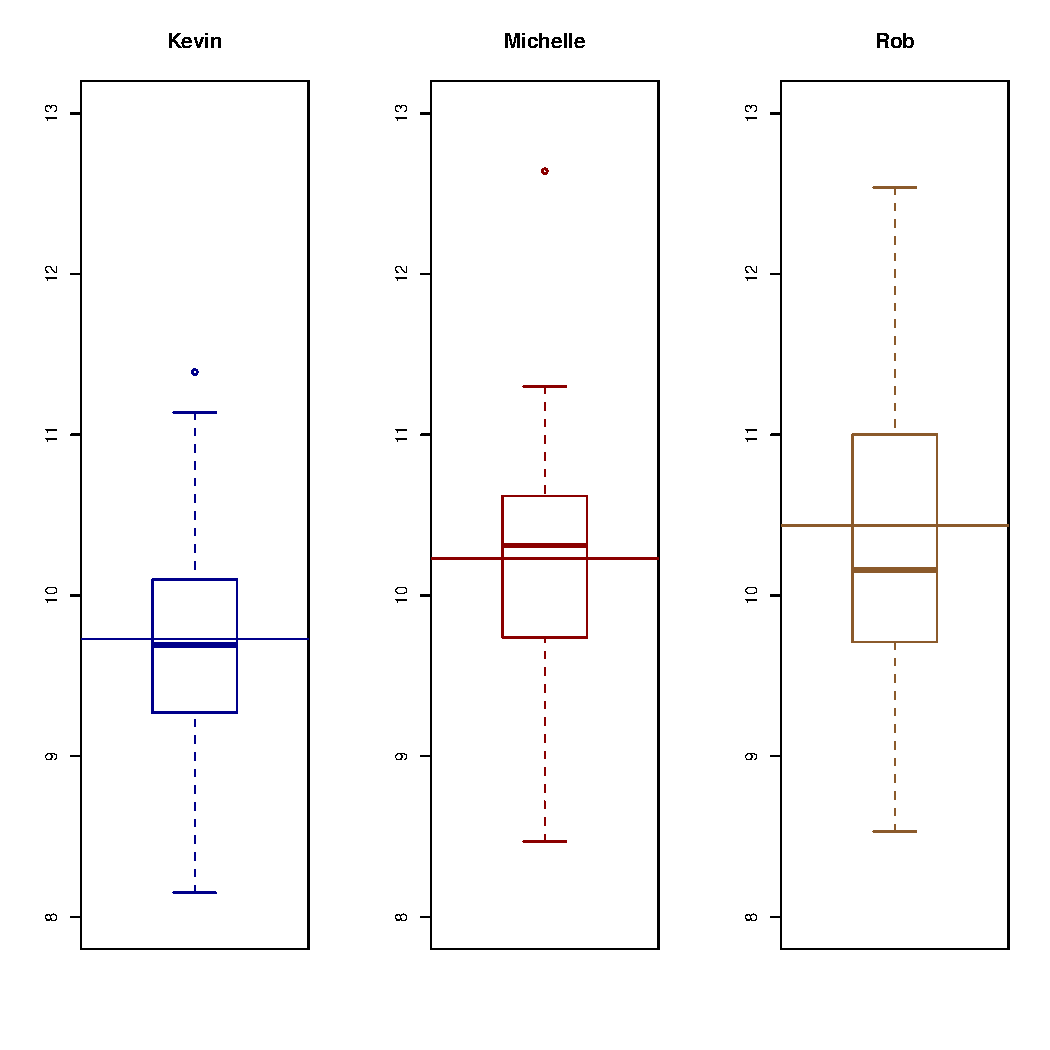
\includegraphics[width=7.5cm]{99_05_bwStrength.pdf}
  \end{center}
\end{frame}

\begin{frame}
  \vspace{0.25cm}
  The p-values of the Anderson-Darling normality test on operators are:
  \begin{itemize}
    \item Rob: 0.371;
    \item Kevin: 0.975;
    \item Michelle: 0.419.
  \end{itemize}
  \vspace{1cm}
  For each $ \alpha $ between those normally used, It is not possible to establish that data don't belong to a normally distributed population.\\
  \vspace{0.5cm}
  It is possible to assert that \textbf{the normality assumption required by ANOVA is satisfied}.
\end{frame}

\begin{frame}
  \vspace{0.25cm}
  One of the assumption of ANOVA is that different groups have variance equal between them. The hypothesis for this test are:\\ 
  $ H_0 $: all operators have the same variance;\\
  $ H_A $: almost one operator has variance different from others.\\
  \vspace{0.5cm}
  Both Bartlett test (p-value = 0.301) and Levene test (p-value = 0.400) show that the variances are not significantly different.\\
  \vspace{0.5cm}
  This fact means that the observed differences in the variances of groups are due to chance alone, so  \textbf{the homoskedasticity assumption required by ANOVA is satisfied}.
\end{frame}

\begin{frame}[fragile]
  \vspace{0.25cm}
  The variance analysis gives the following result:
  \begin{verbatim}
             Df  Sum Sq  Mean Sq  F value  p value  
Operator     2    6.621   3.3104   3.8508  0.02577
Residuals   72   61.895   0.8597  
  \end{verbatim}
  F test is the ratio between MS of Operatore factor and residuals (or error).\\
  \vspace{0.25cm}
  An $ F $ value close to 1 means that the differences in the averages of the factors are not significant but they can be due to chance.\\
  \vspace{0.25cm}
  The ratio $ F $ is distributed as a random variable F with 2 and 72 degrees of freedom.\\
\end{frame}

\begin{frame}
  \vspace{0.75cm}
  The p-value is 2.577\%.  It gives different conclusion according to the fixed significance level $ \alpha $:
  \vspace{0.5cm}
  \begin{itemize}
    \item The null hypothesis asserts that the averages are all equal and the alternative hypothesis asserts that \textbf{at least one of the averages is different}. Considering a 5\% confidence level, the null hypothesis $ H_0 $ is rejected;
    \vspace{0.5cm}
    \item Considering a 1\% confidence level, instead, the null hypothesis is not rejected. The conclusion is that the averages are  \textbf{statistically equal to each other}.
  \end{itemize}
\end{frame}

\begin{frame}
  \vspace{1cm}
  Since, at least for $ \alpha = 0.05 $, the averages of the groups seem to be all equal to each other, It can be useful apply the contrasts to analyse the differences between different operators.\\ 
  \vspace{1cm}
  It only makes sense if Rob, Kevin e Michelle are the only operators of the company and so we are applying a \textbf{fixed effects ANOVA}.
\end{frame}

\begin{frame}
  Graphical check of the model:\\
  \vspace{.1cm}
  \begin{center}
    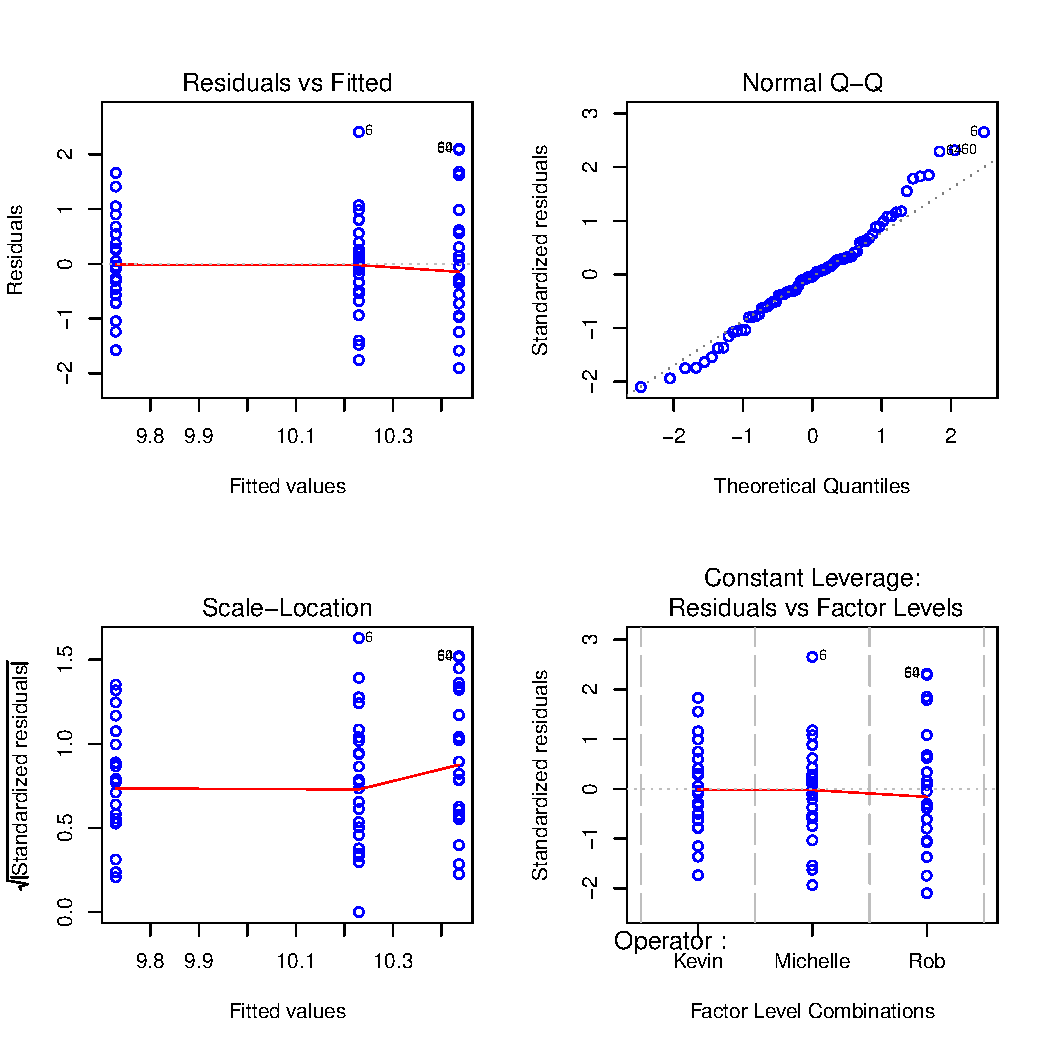
\includegraphics[width=7.5cm]{99_05_residAnovaCarseat}
    \end{center}
\end{frame}

\livelloB{Multi-head machine}

\begin{frame}
  \begin{description}
    \item[Data: ]pencap.txt \\ 
    \item[Description: ]
      \begin{footnotesize}
        \begin{itemize}
          \item \textit{Cavity}: indicates the number of head (factor);
          \item \textit{Width}: indicates the measurement (in mm).
        \end{itemize}
      \end{footnotesize}
    \item[Aims: ]
      \begin{footnotesize}
        A society that produces ballpoint pens uses a multi-head machine for the production of caps for pens. The productor wants to compare the means and the variances on all 16 heads and to determine if there are variations on the means of the different heads.
        \begin{itemize}
          \item[-] Let us show the BW plot of \textit{Width} for each head.
          \item[-] Let us check if different groups belong to a normally distributed population.
          \item[-] Let us check if the different groups have the same variance (homoskedasticity).
          \item[-] Let us check if there are differences between the means of the different groups.
        \end{itemize}
      \end{footnotesize}
  \end{description}
\end{frame}

\begin{frame}
  B-W Graph of \textit{Width} separately for each head:\\
  \vspace{-0.5cm}
  \begin{center}
    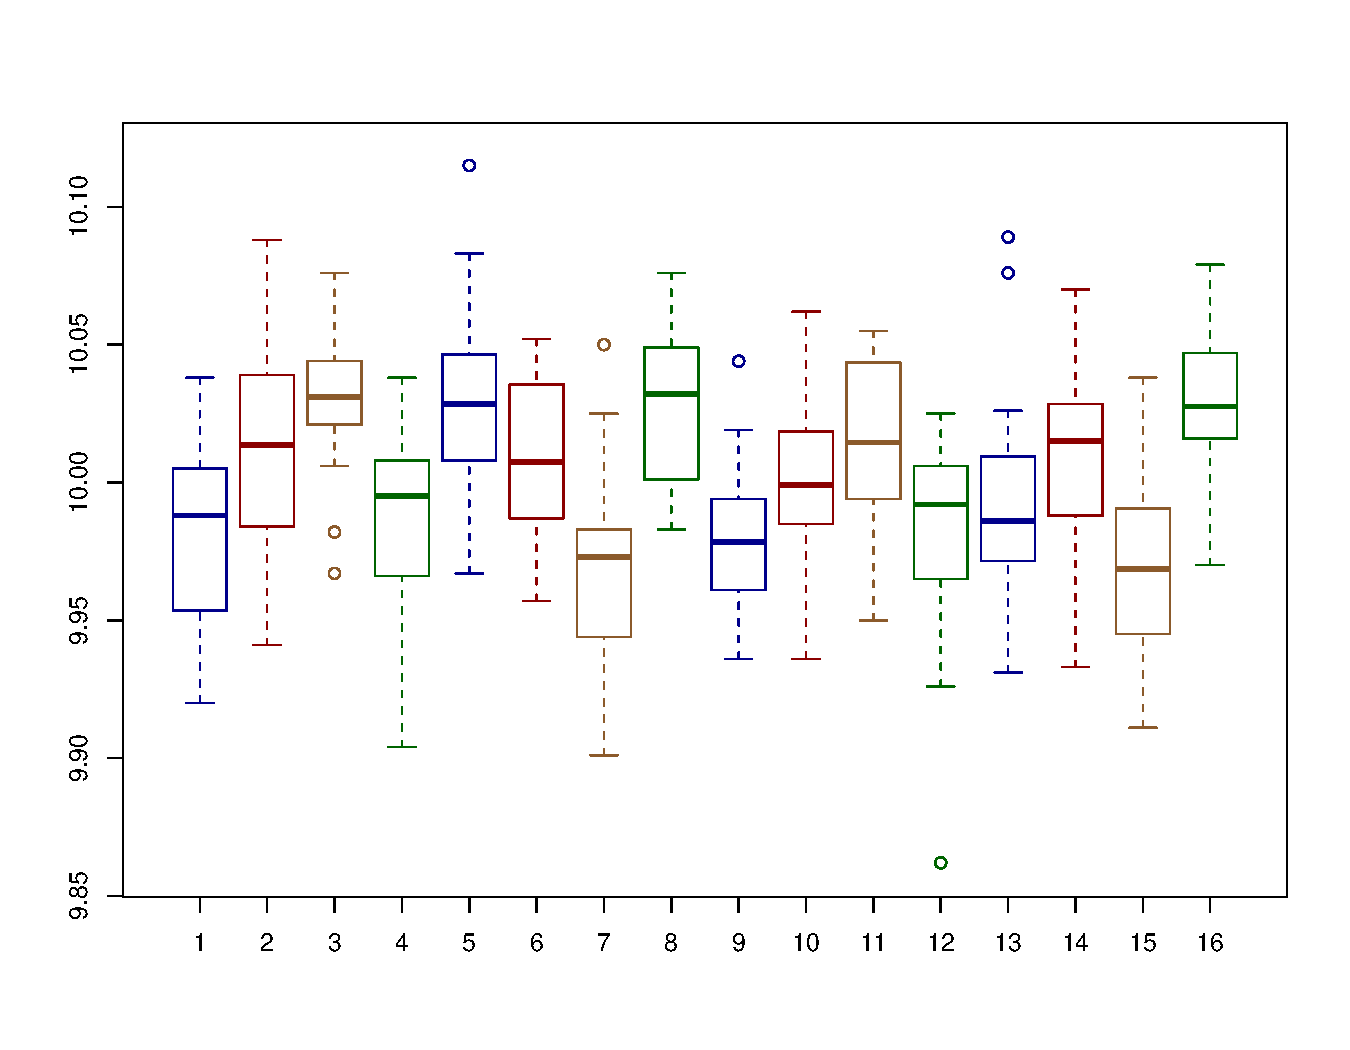
\includegraphics[width=11cm]{99_05_bwPencap.pdf}
  \end{center}
\end{frame}

\begin{frame}
  \begin{minipage}[t]{0.48\textwidth}
    Normality\\

    \vspace*{0.25cm}
    Anderson-Darling Test:
    \begin{table}[ht]
      \begin{tiny}
        \begin{tabular}{lr}
          \hline
          Cavity & p value \\ 
          \hline
           1 & 0.2155 \\ 
           2 & 0.9142 \\ 
           3 & 0.3541 \\ 
           4 & 0.1333 \\ 
           5 & 0.5674 \\ 
           6 & 0.3454 \\ 
           7 & 0.2569 \\ 
           8 & 0.5680 \\ 
           9 & 0.8530 \\ 
          10 & 0.6430 \\ 
          11 & 0.5147 \\ 
          12 & 0.0264 \\ 
          13 & 0.0845 \\ 
          14 & 0.5149 \\ 
          15 & 0.5856 \\ 
          16 & 0.2628 \\ 
          \hline
        \end{tabular}
      \end{tiny}
    \end{table}
  \end{minipage}
  \hfill
  \begin{minipage}[t]{0.48\textwidth}
    Homoskedasticity of variances\\

    \vspace*{0.25cm}
    Bartlett Test:\\
    \texttt{p value: 0.726}\\

    \vspace*{0.75cm}
    Levene Test:\\
    \texttt{p value: 0.899}\\
  \end{minipage}
\end{frame}

\begin{frame}[fragile]
  \vspace{0.25cm}
  Variance analysis:
  \begin{verbatim}
             Df  Sum Sq   Mean Sq F value   p value    
Cavity       15 0.14199 0.0094659  8.3501 5.922e-16
Residuals   304 0.34462 0.0011336    
  \end{verbatim}
\end{frame}

\begin{frame}
  Graphical check of the model:\\
  \vspace{.1cm}
  \begin{center}
    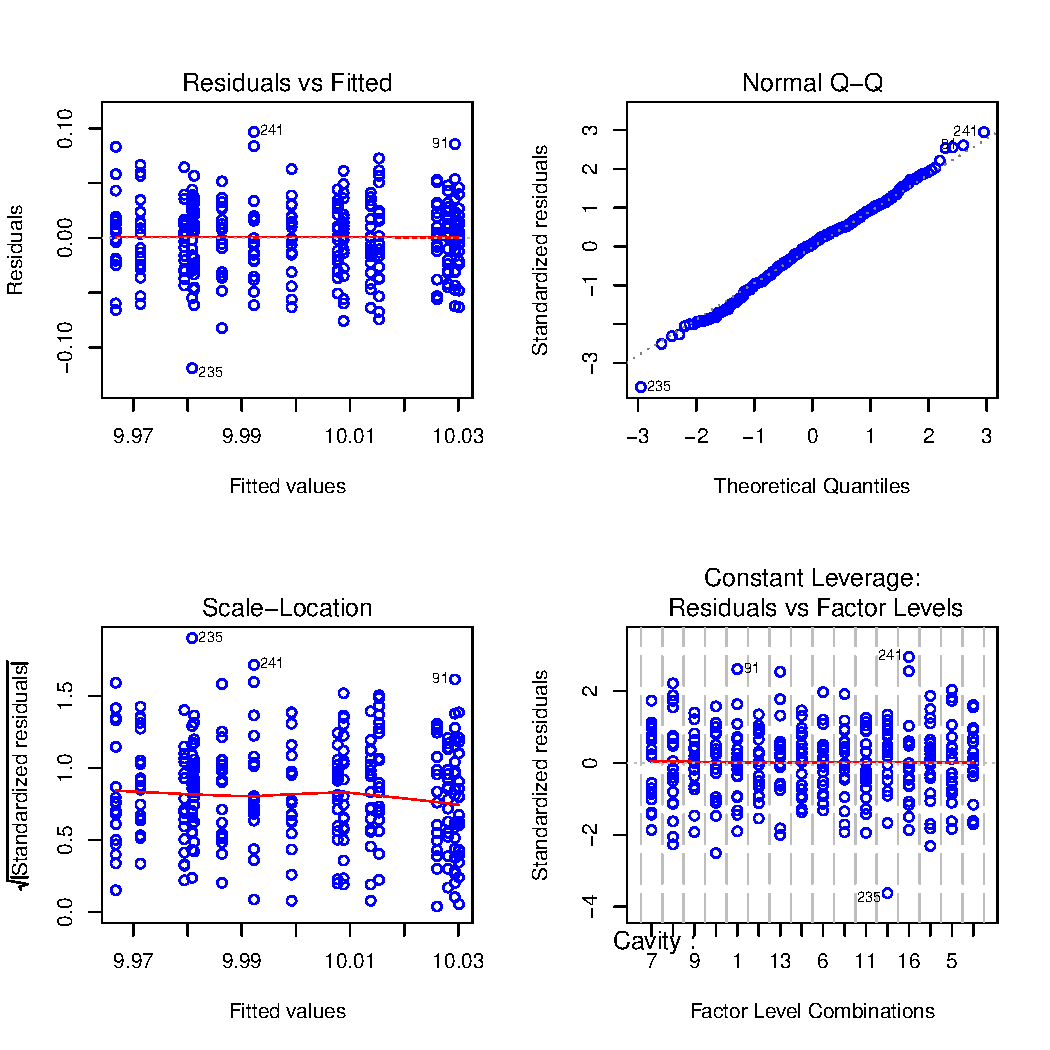
\includegraphics[width=7.5cm]{99_05_residAnovaPencap}
    \end{center}
\end{frame}

\livelloB{Tear resistance}

\begin{frame}
  \begin{description}
    \item[Data: ]sturdy.txt \\ 
    \item[Description: ]
      \begin{footnotesize}
        \begin{itemize}
          \item \textit{Time}: indicates the time between the solicitation and the tear (in minutes);
          \item \textit{Group}: indicates the raincoats brand (factor).
        \end{itemize}
      \end{footnotesize}
    \item[Aims: ]
      \begin{footnotesize}
        The aim is to study the tear resistance of five different raincoats brand. The raincoats were subjected to the same solicitation, and the time between the solicitation and the tear (in minutes and in decimal fractions of a minute) was measured.   
        \begin{itemize}
          \item[-] Let us show the BW plot of \textit{Time} for each brand.
          \item[-] Let us check that different groups belong to a normally distributed population.
          \item[-] Let us check if the different groups have the same variance (homoskedasticity).
          \item[-] Let us check if there are differnces between thwe means of the different groups.
        \end{itemize}
      \end{footnotesize}
  \end{description}
\end{frame}

\begin{frame}
  B-W Graph of \textit{Time} separately for each brand:\\
  \vspace{-0.5cm}
  \begin{center}
    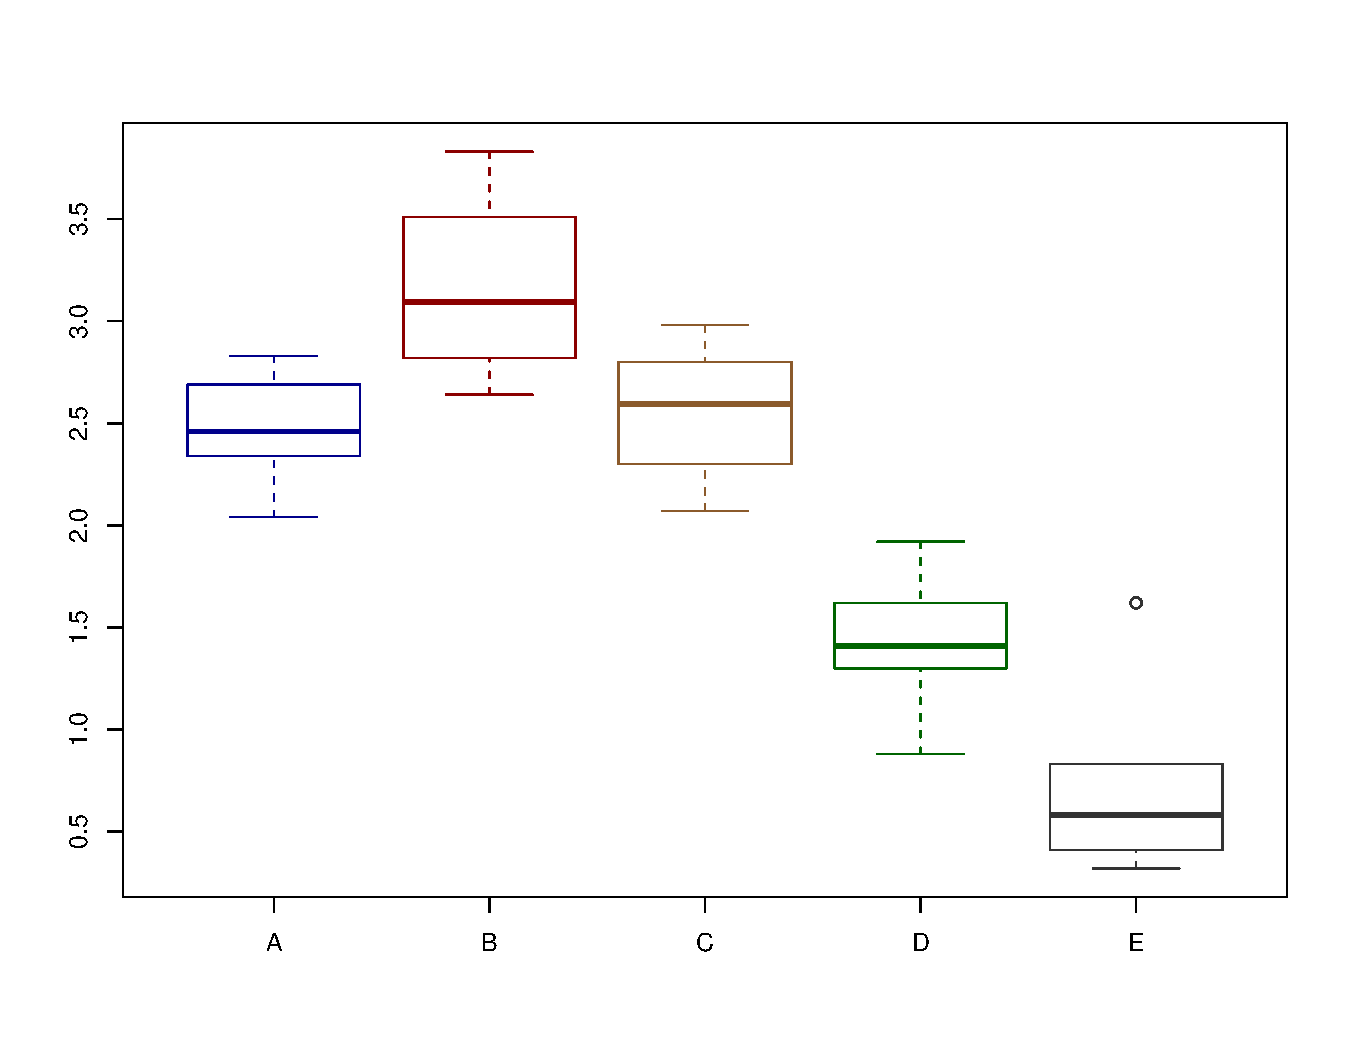
\includegraphics[width=11cm]{99_05_bwSturdy.pdf}
  \end{center}
\end{frame}

\begin{frame}
  Normality\\
  \vspace*{0.25cm}
  Because of the low number of units within each groups, It is not possible to perform Anderson Darling test. However, analysing the B-W plot of the previous slide, the normality assumption is considered valid. \\ 
  \vspace{1cm}
  Homoskedasticity of variances\\
  \vspace*{0.25cm}
  Bartlett Test\\
  \texttt{p value: 0.7722}\\
  \vspace*{0.75cm}
  Levene Test\\
  \texttt{p value: 0.9214}\\
\end{frame}

\begin{frame}[fragile]
  \vspace{0.25cm}
  Variance analysis:
  \begin{verbatim}
            Df  Sum Sq Mean Sq F value   p value    
Group        4 18.1681  4.5420  28.261 3.475e-08
Residuals   21  3.3751  0.1607       
  \end{verbatim}
\end{frame}

\begin{frame}
  Graphical check of the model:\\
  \vspace{.1cm}
  \begin{center}
    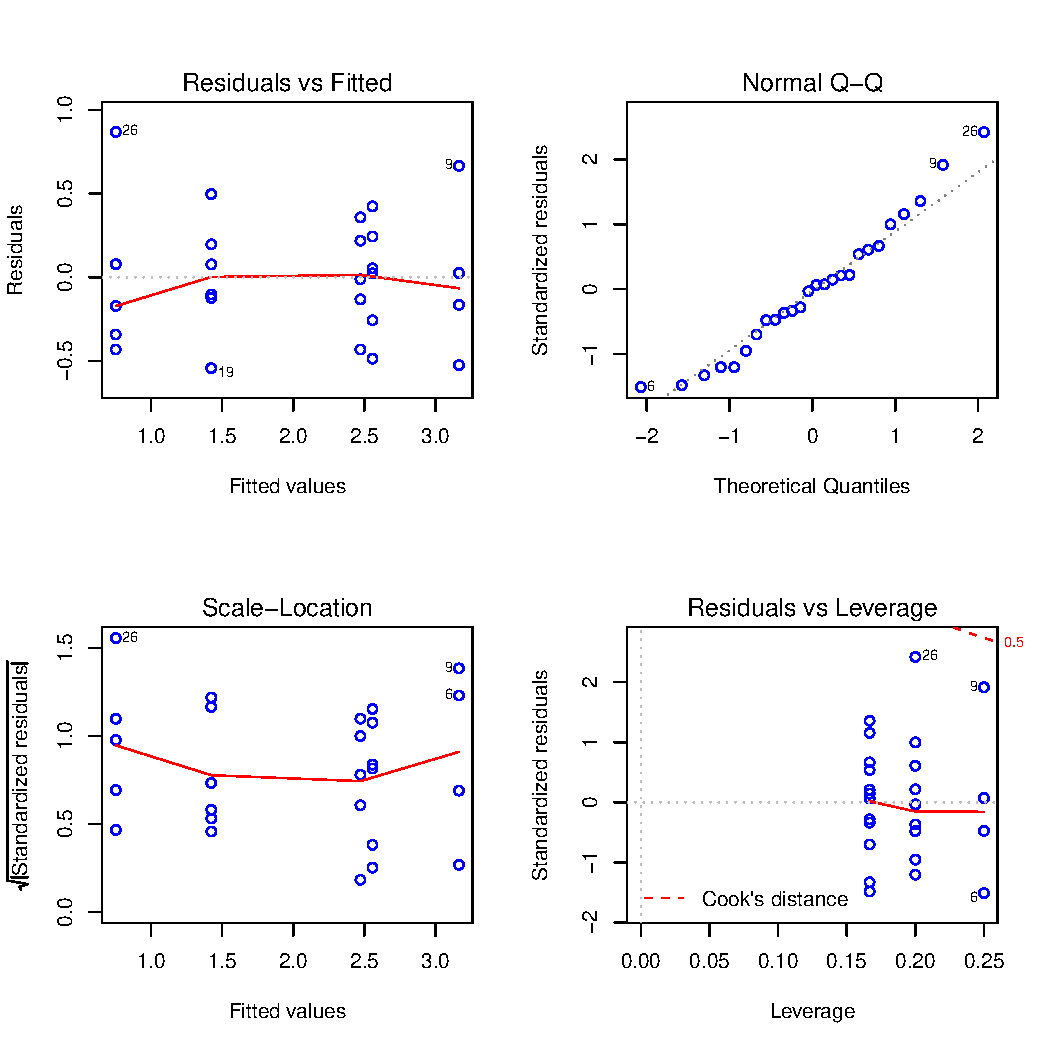
\includegraphics[width=7.5cm]{99_05_residAnovaSturdy}
    \end{center}
\end{frame}

\livelloB{Effect of toxic agent}

\begin{frame}
  \begin{description}
    \item[Data: ]rats.txt \\ 
    \item[Description: ]
      \begin{footnotesize}
        \begin{itemize}
          \item \textit{Time}: identifies the survival time (in tens of hours);
          \item \textit{Poison}: identifies the poison type (factor);
          \item \textit{Treatment}: identifies the type of treatment (factor).
        \end{itemize}
      \end{footnotesize}
    \item[Aims: ]
      \begin{footnotesize}
        The aim is to study the survival time to different types of rats treatments to which has been administered the second type of poison.  
        \begin{itemize}
          \item[-] Let us show the BW plot of \textit{Time} for each treatment.
          \item[-] Let us check if the different groups belong to a normally distributed population.
          \item[-] Let us check if the different groups have the same variance (homoskedasticity).
          \item[-] Is It posible to make a comparison? How?
        \end{itemize}
      \end{footnotesize}
  \end{description}
\end{frame}

\begin{frame}
  B-W Graph of \textit{Time} separately for each treatment:\\
  \vspace{-0.5cm}
  \begin{center}
    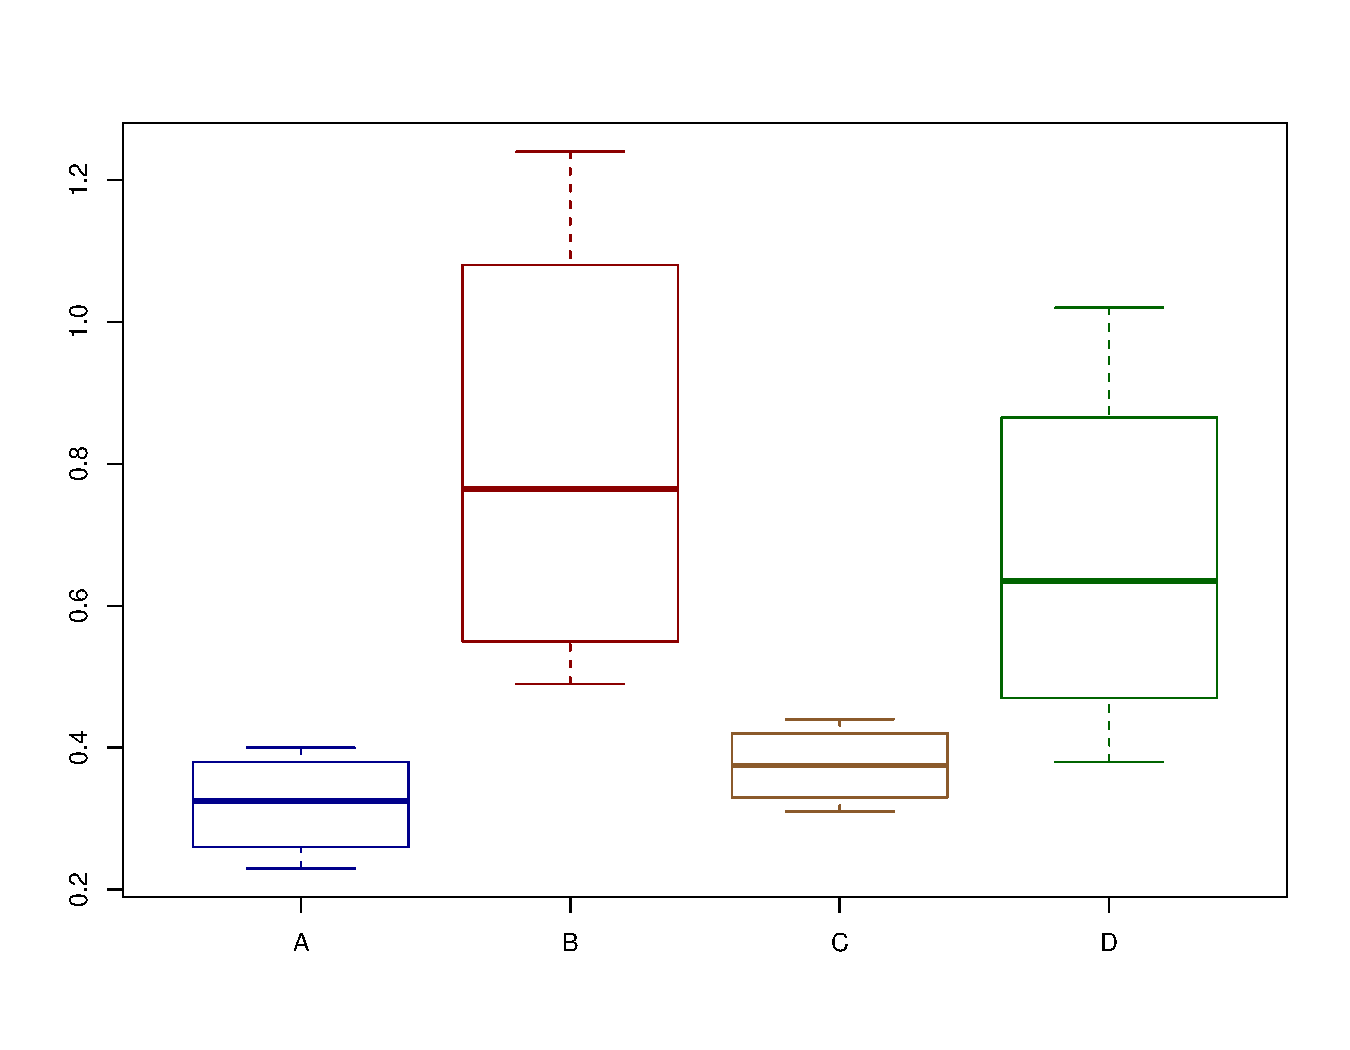
\includegraphics[width=11cm]{99_05_bwTreatment.pdf}
  \end{center}
\end{frame}

\begin{frame}
  Normality\\
  \vspace*{0.25cm}
  Because of the low number of units within each group, It is not possible to perform Anderson Darling test. However, analysing the B-W plot of the previous slide, the normality assumption is considered valid. \\ 
  \vspace{1cm}
  Homoskedasticity of variances\\
  \vspace*{0.25cm}
  Bartlett Test - \texttt{p value: 0.0229}\\
  Levene Test - \texttt{p value: 0.0373}\\
  \vspace*{0.75cm}
  The homoskedasticity hypothesis is rejected with a 5\% confidence level.
\end{frame}

\begin{frame}
  B-W graph of the reciprocal of \textit{Time} for each treatment:\\
  \vspace{-0.5cm}
  \begin{center}
    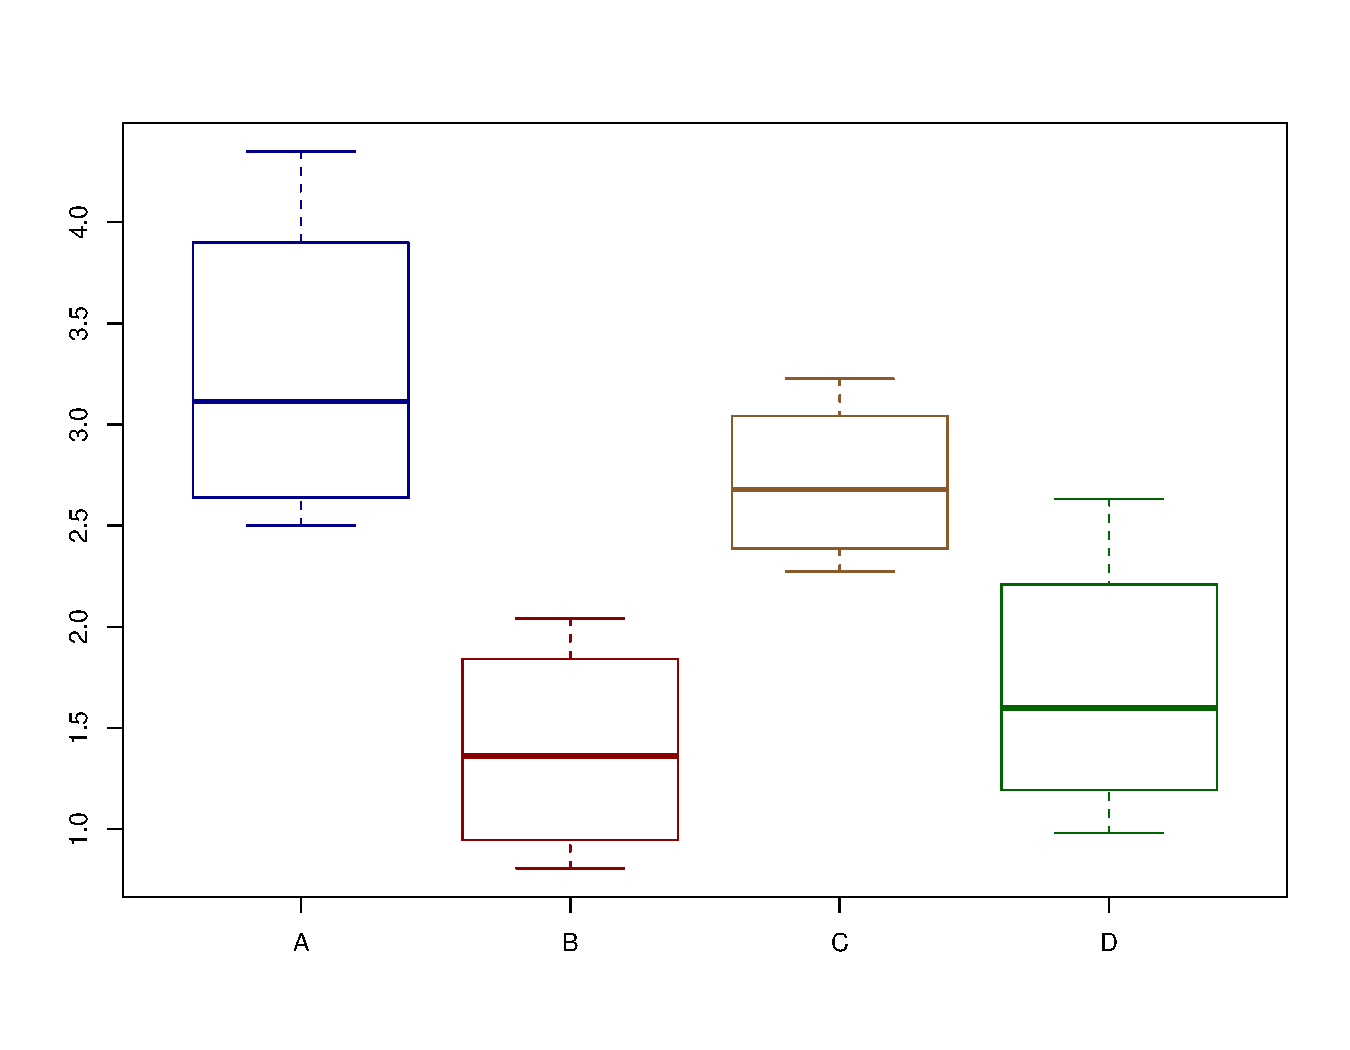
\includegraphics[width=11cm]{99_05_bwInvTreatment.pdf}
  \end{center}
\end{frame}

\begin{frame}
  Normality\\
  \vspace*{0.25cm}
  Because of the low number of units within each group, It is not possible to perform Anderson Darling test. However, analysing the B-W plot of the previous slide, the normality assumption is considered valid. \\ 
  \vspace{1cm}
  Homoskedasticity of variances\\
  \vspace*{0.25cm}
  Bartlett Test:\\
  \texttt{p value: 0.7337}\\
  \vspace*{0.75cm}
  Levene Test:\\
  \texttt{p value: 0.6244}\\
\end{frame}

\begin{frame}[fragile]
  \vspace{0.25cm}
  Variance analysis:
  \begin{verbatim}  
            Df Sum Sq Mean Sq F value  p value  
Treatment    3 9.1424 3.04747  7.3913 0.004594
Residuals   12 4.9477 0.41231       
  \end{verbatim}
\end{frame}

\begin{frame}
   Graphical check of the model:\\
  \vspace{.1cm}
  \begin{center}
    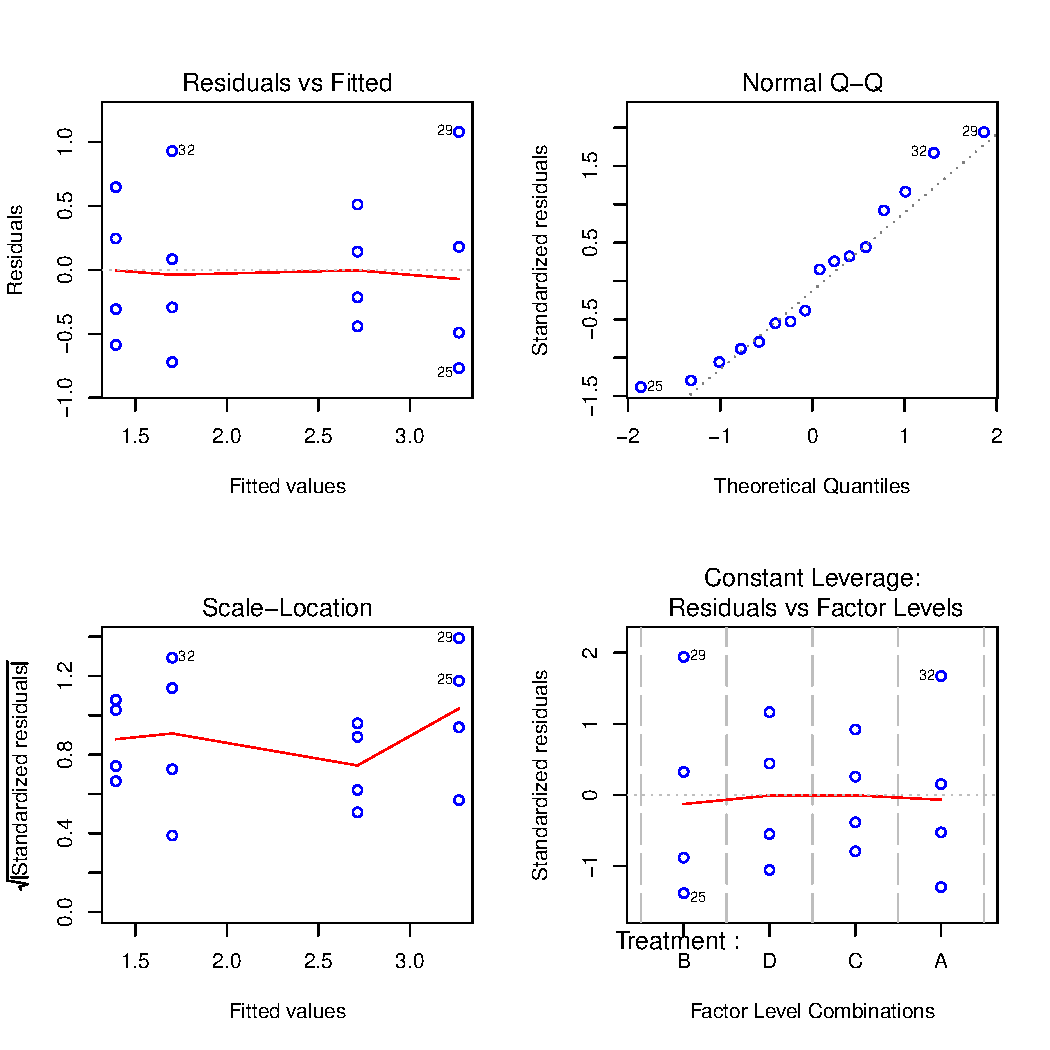
\includegraphics[width=7.5cm]{99_05_residAnovaInvTreatment}
    \end{center}
\end{frame}



\livelloA{Multi-factor variance analysis}

\livelloB{Stopping distance of a car on wet road}

\begin{frame}
  \begin{description}
    \item[Data: ]brakedis.txt \\ 
    \item[Description: ]
      \begin{footnotesize}
        \begin{itemize}
          \item \textit{Tire}: identifies the tyre model (factor);
          \item \textit{Tread}: identifies the tread depth, 1.5 or 10.0 mm (factor);
          \item \textit{ABS}: indicates whether the ABS is in operation (factor);
          \item \textit{Distance}: indicates the distance traveled, on wet surfaces, by the vehicle before stopping (in meters). 
        \end{itemize}
      \end{footnotesize}
    \item[Aims: ]
      \begin{footnotesize}
        The engineers want to know if the distance traveled by a car on wet surfaces is influenced by the tyre model, by the wear of the tread, the operation or not of the ABS. Data are collected with the same car at the speed of 60 km/h before braking.
      \begin{itemize}
          \item[-] Let us check which factors influence the stopping distance on wet surfaces.
        \end{itemize}
      \end{footnotesize}
  \end{description}
\end{frame}

\begin{frame}[fragile]
  \vspace{0.25cm}
  The first model analysed includes all factors and all possible interactions. The model is indicated in the following way:
  $ Distance = Tire \; | \; Tread \; | \; ABS $.\\
  The variance analysis produces the following result:
  \begin{verbatim}
               Df  Sum Sq Mean Sq F value   p value    
Tire            2  37.316  18.658  9.4074  0.003488
Tread           1   0.107   0.107  0.0538  0.820517    
ABS             1 140.167 140.167 70.6723 2.255e-06
Tire:Tread      2   6.656   3.328  1.6779  0.227740    
Tread:ABS       1   1.215   1.215  0.6126  0.448979    
Tire:ABS        2   2.986   1.493  0.7527  0.492074    
Tire:Tread:ABS  2   2.572   1.286  0.6485  0.540199    
Residuals      12  23.800   1.983 
  \end{verbatim}
\end{frame}

\begin{frame}[fragile]
  \vspace{0.25cm}
  Only two coefficient of the previous model are significant.\\ 
  \vspace{0.5cm}
  By eliminating a term at a time, starting from that with the higher p-value, we arrive at the following reduced model:
  \begin{verbatim}
            Df  Sum Sq Mean Sq F value   p value 
Tire         2  37.316  18.658  9.9946 0.0009792
ABS          1 140.167 140.167 75.0843 3.322e-08
Residuals   20  37.336   1.867  
  \end{verbatim}
  So, It is possible to conclude that the stopping distance is influenced by the tyre model and by the operation of ABS.
\end{frame}

\begin{frame}
   Graphical check of the model:\\
  \vspace{.1cm}
  \begin{center}
    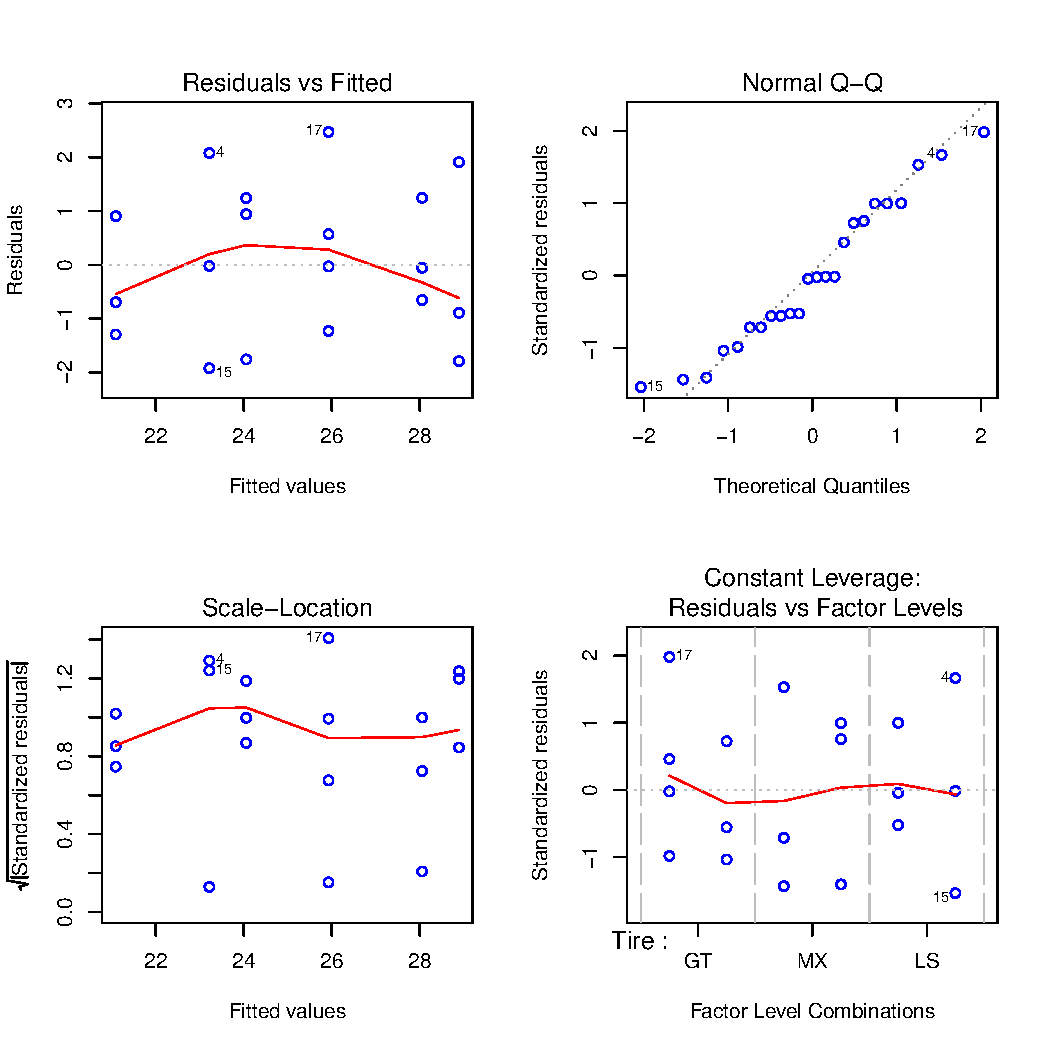
\includegraphics[width=7.5cm]{99_05_residAnovaBrakedis}
    \end{center}
\end{frame}

\livelloB{Wine quality}

\begin{frame}
  \begin{description}
    \item[Data: ]rioja.txt \\ 
    \item[Description: ]
      \begin{footnotesize}
        \begin{itemize}
          \item \textit{Judge}: indicates the name of the taster (factor);
          \item \textit{Wine}: indicates the wine name (factor);
          \item \textit{Trial}: indicates the order of tasting;
          \item \textit{Score}: indicates the evaluation reached (score).
        \end{itemize}
      \end{footnotesize}
    \item[Aims: ]
      \begin{footnotesize}
        A society wants to determine if there are significant differences in the quality of three types of wine: Matador, Conquistador e Saeta. Ten judges have assigned a score to the wine tasted. The order of tasting was random.
      \begin{itemize}
          \item[-] Let us perform a variance analysis to check if the mean of the score is equal for all types of wine.
          \item[-] Let us perform a variance analysis to check if the mean of the score is equal for all the judges.
          \item[-] Let us perform a variance analysis to check if the mean of the score depends by the type of wine and by the judge.
        \end{itemize}
      \end{footnotesize}
  \end{description}
\end{frame}

\begin{frame}
  B-W Graph of \textit{Score} separately for each type of wine:\\
  \begin{center}
    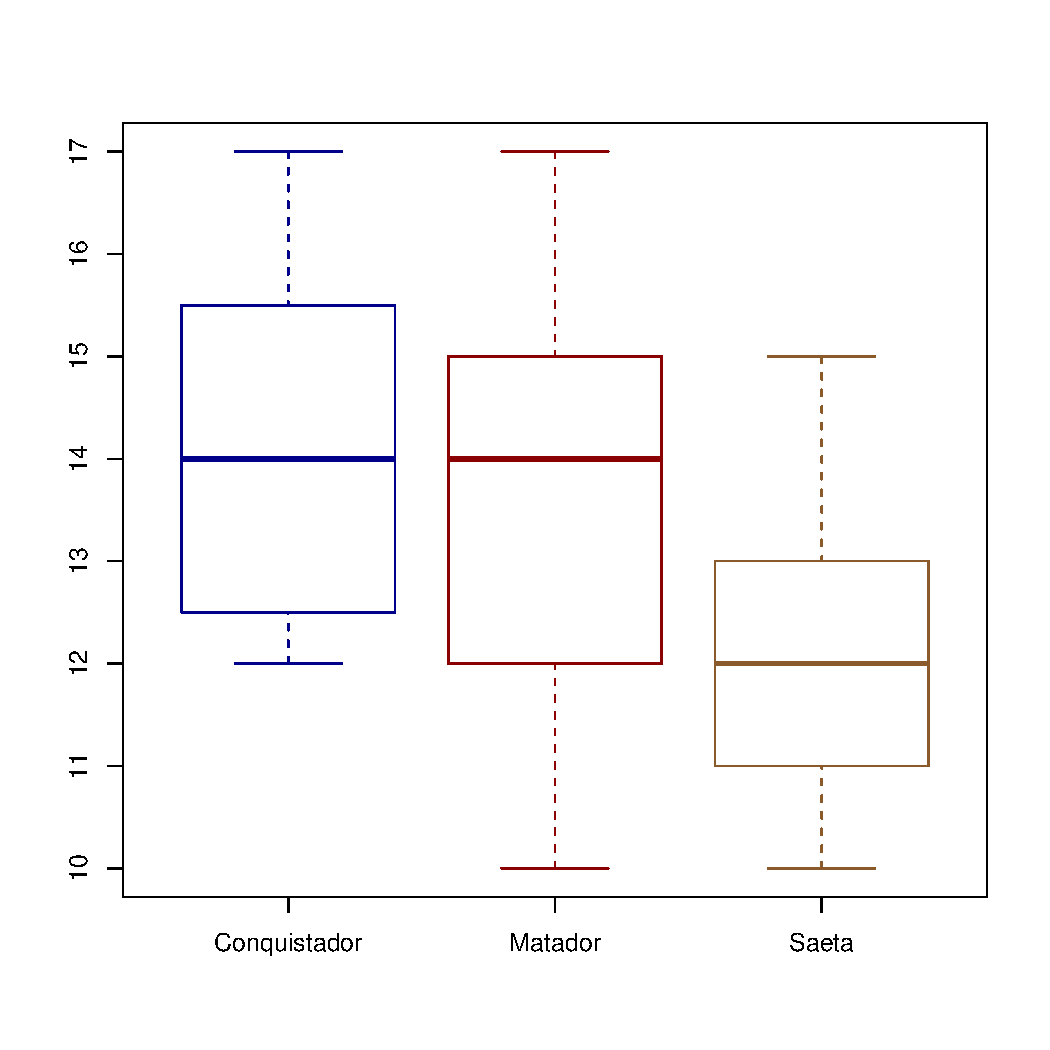
\includegraphics[width=7.5cm]{99_05_bwWine.pdf}
  \end{center}
\end{frame}

\begin{frame}
  B-W Graph of \textit{Score} separately for each judge:\\
  \vspace{-1cm}
  \begin{center}
    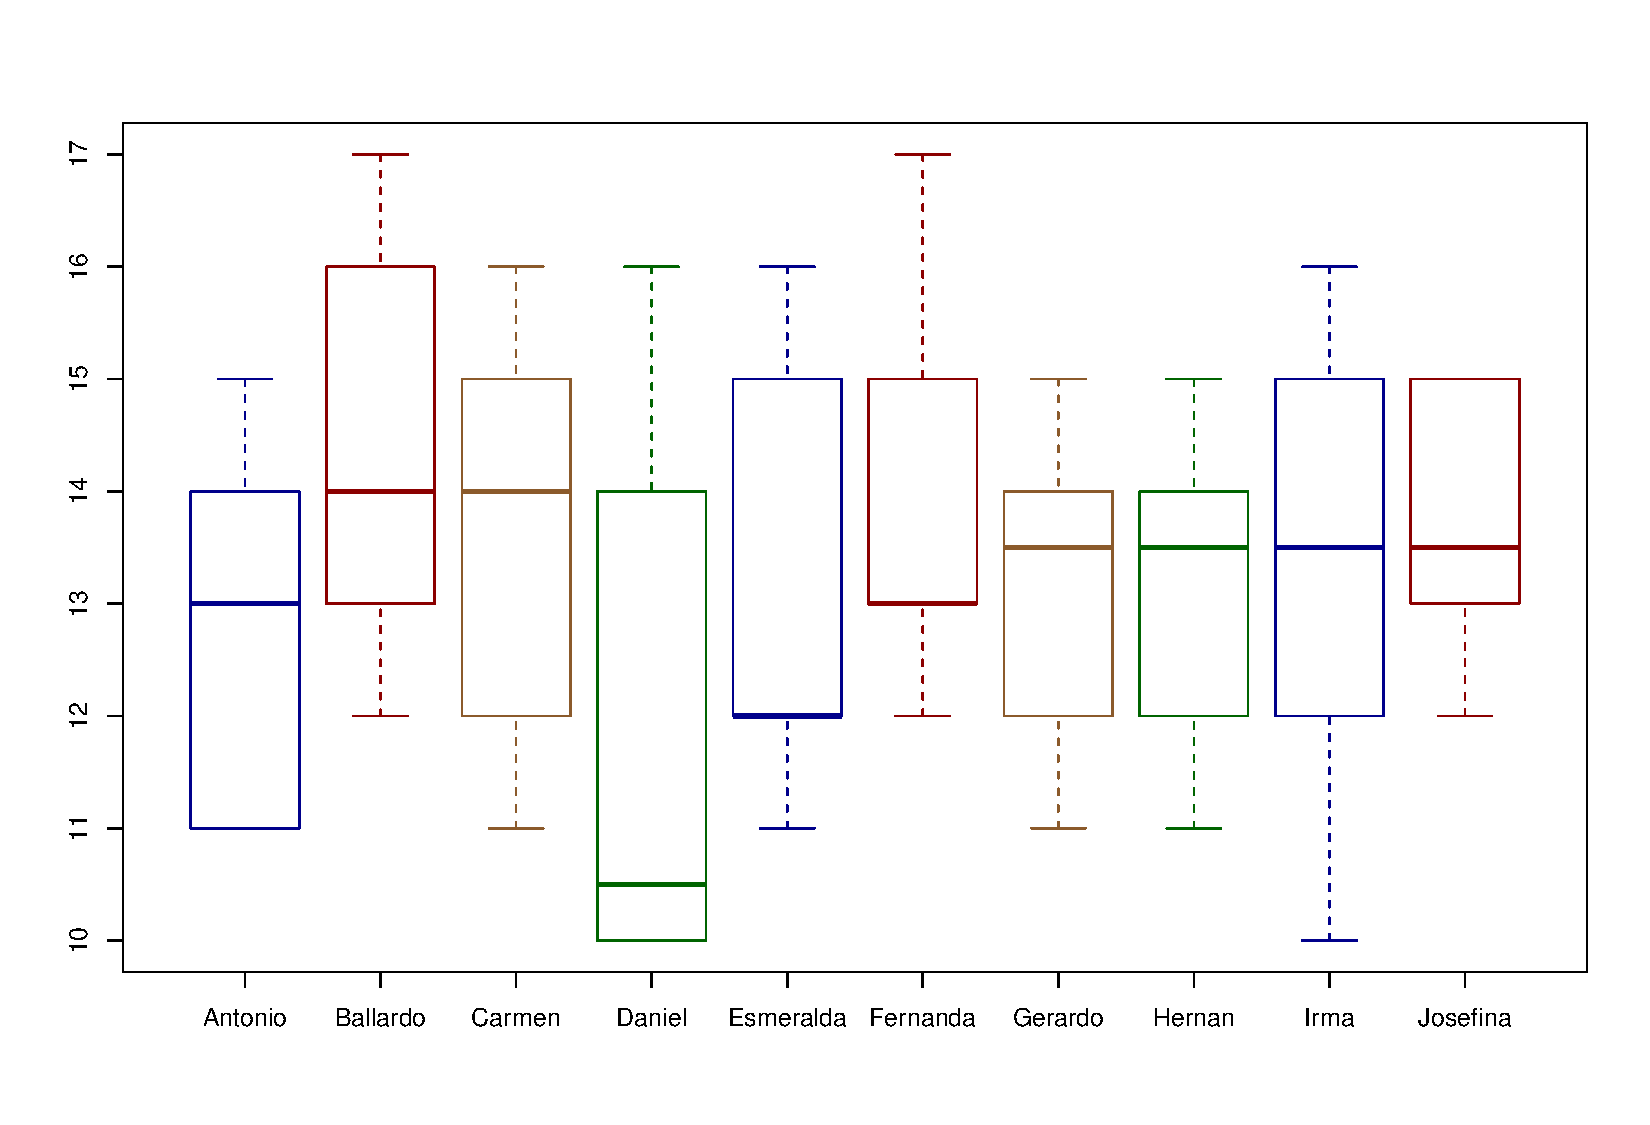
\includegraphics[scale=0.45]{99_05_bwJudge.pdf}
  \end{center}
\end{frame}

\begin{frame}
  Homoskedasticity of variances\\
  \vspace{0.5cm}
  \begin{minipage}[t]{0.48\textwidth}
    For each type of wine:\\

    \vspace*{0.25cm}
    Bartlett Test:\\
    \texttt{p value: 0.5726}\\

    \vspace*{0.75cm}
    Levene Test:\\
    \texttt{p value: 0.6283}\\
  \end{minipage}
  \hfill
  \begin{minipage}[t]{0.48\textwidth}
    For each judge:\\

    \vspace*{0.25cm}
    Bartlett Test:\\
    \texttt{p value: 0.9267}\\

    \vspace*{0.75cm}
    Levene Test:\\
    \texttt{p value: 0.9763}\\
  \end{minipage}
\end{frame}

\begin{frame}[fragile]
  \vspace{0.25cm}
  Variance analysis:
  \begin{verbatim}
            Df Sum Sq Mean Sq  F value   p value  
Wine         2  39.433 19.7167  7.0794 0.001794
Residuals   57 158.750  2.7851   
  \end{verbatim}
\end{frame}

\begin{frame}
   Graphical check of the model:\\
  \vspace{.1cm}
  \begin{center}
    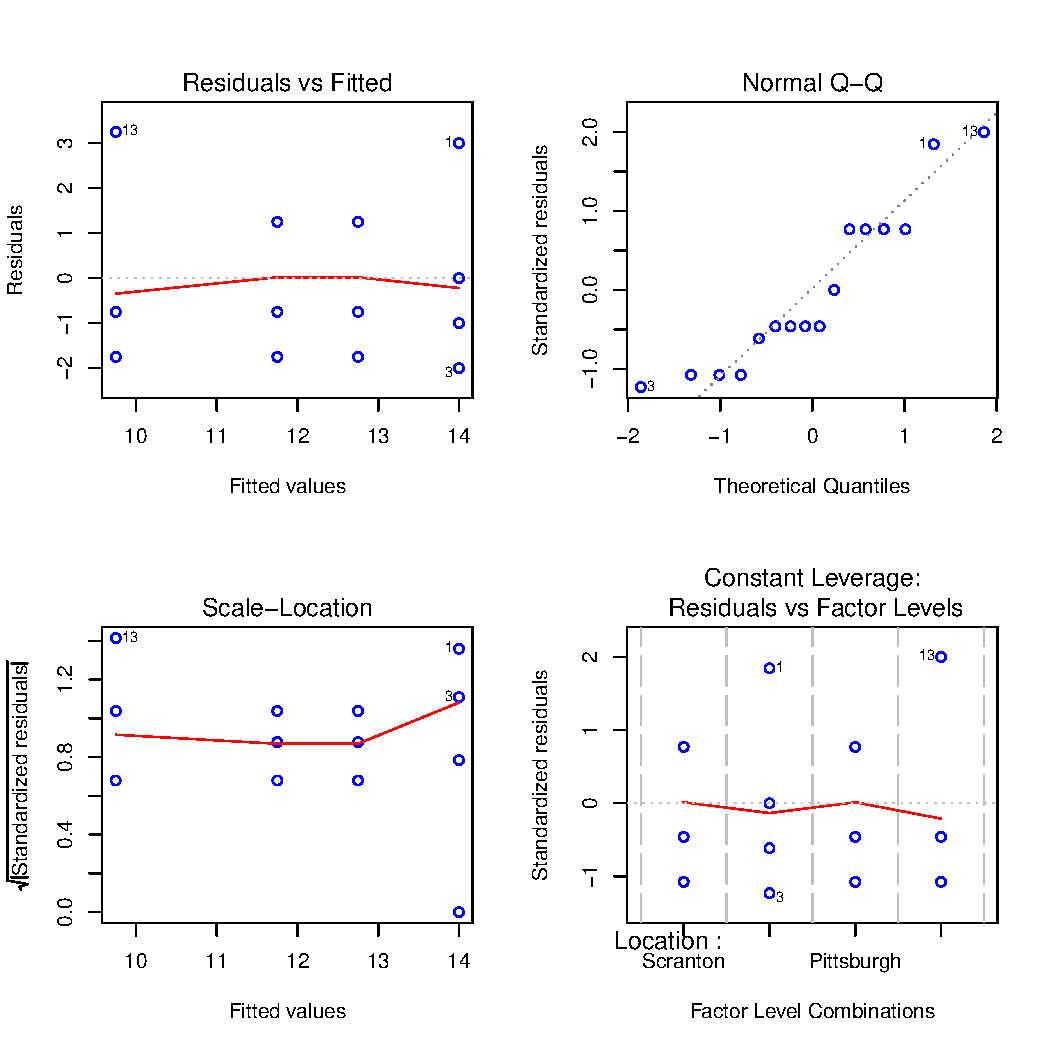
\includegraphics[width=7.5cm]{99_05_residAnovaPntWear1}
    \end{center}
\end{frame}

\begin{frame}[fragile]
  \vspace{0.25cm}
  Variance analysis:
  \begin{verbatim}
            Df Sum Sq Mean Sq  F value p value  
Judge        9  24.683  2.7426  0.7904 0.6264
Residuals   50 173.500  3.4700    
  \end{verbatim}
\end{frame}

\begin{frame}
   Graphical check of the model:\\
  \vspace{.1cm}
  \begin{center}
    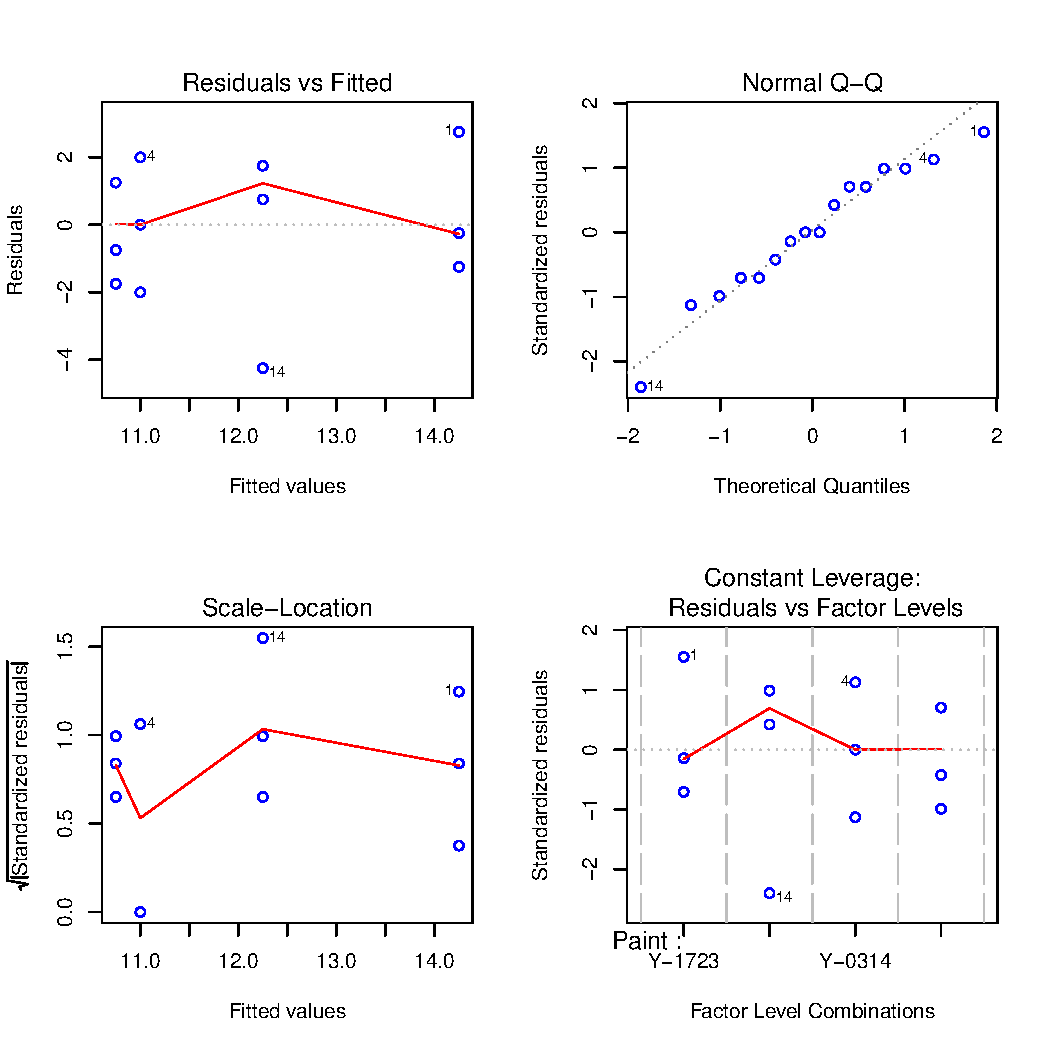
\includegraphics[width=7.5cm]{99_05_residAnovaPntWear2}
    \end{center}
\end{frame}

\begin{frame}[fragile]
  \vspace{0.25cm}
  Variance analysis:
  \begin{verbatim}
            Df Sum Sq Mean Sq  F value  p value   
Wine         2  39.433 19.7167  7.0592 0.002054
Judge        9  24.683  2.7426  0.9819 0.466912   
Residuals   48 134.067  2.7931    
  \end{verbatim}
\end{frame}

\begin{frame}
   Graphical check of the model:\\
  \vspace{.1cm}
  \begin{center}
    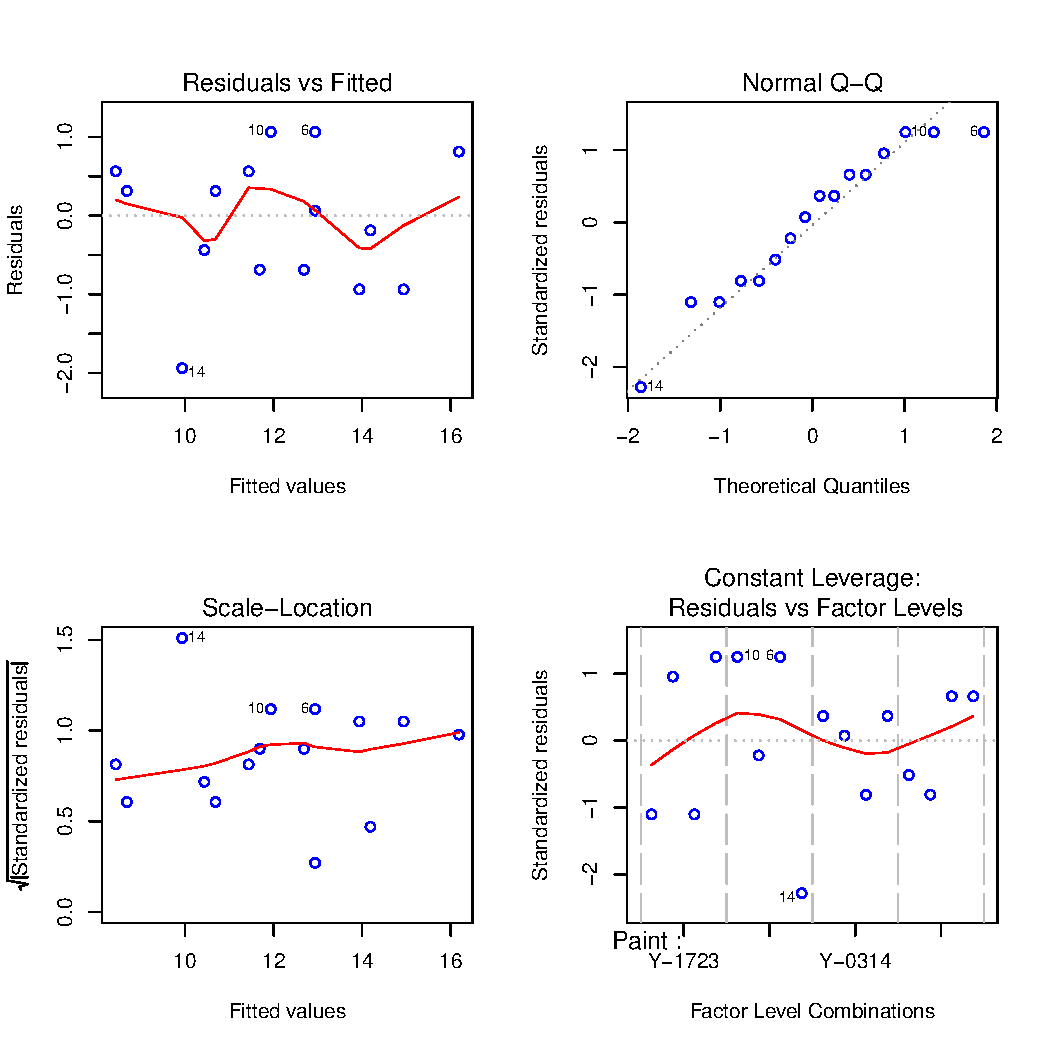
\includegraphics[width=7.5cm]{99_05_residAnovaPntWear3}
    \end{center}
\end{frame}

\livelloB{Wear of paint}

\begin{frame}
  \begin{description}
    \item[Data: ]pntwear.txt \\ 
    \item[Description: ]
      \begin{footnotesize}
        \begin{itemize}
          \item \textit{Location}: indicates the place of the test (factor);
          \item \textit{Paint}: indicates the type of paint (factor);
          \item \textit{PntWear}: indicates the wear of paint (score).
        \end{itemize}
      \end{footnotesize}
    \item[Aims: ]
      \begin{footnotesize}
        Pennsylvania Department of Transportation is studying the use of four different types of yellow paint for the street. The test is performed on the streets of Philadelphia, Pittsburgh, Harrisburg e Scranton, in Pennsylvania. After a period of exposure to the weather conditions and to the  traffic, the wear of paint is measured in the four cities. For the classification, a higher score was given to a lower wear of the paint. 
      \begin{itemize}
          \item[-] Let us perform an analysis of variance to check if the mean of the wear of the paint is equal for the four cities. 
          \item[-] Let us perform an analysis of variance to check if the mean of the wear of the paint is equal for the four types of paint. 
          \item[-] Let us perform an analysis of variance to check if the mean of the wear of the paint is different between the place and the type of paint.
        \end{itemize}
      \end{footnotesize}
  \end{description}
\end{frame}

\begin{frame}
  B-W Graph of \textit{PntWear} separately for each place:\\
  \begin{center}
    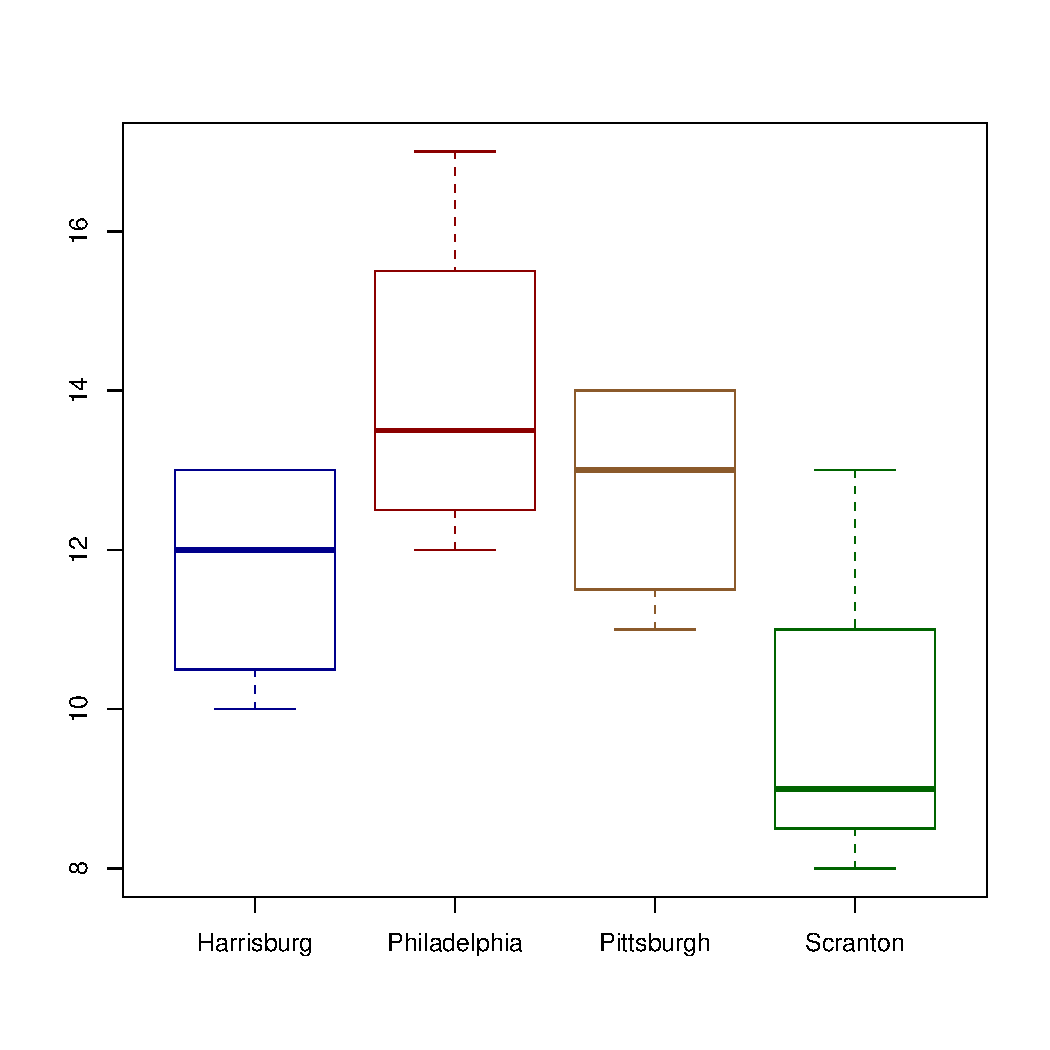
\includegraphics[width=7.5cm]{99_05_bwLocation.pdf}
  \end{center}
\end{frame}

\begin{frame}
  B-W Graph of \textit{PntWear} separately for each type of paint:\\
  \begin{center}
    \includegraphics[width=7.5cm]{99_05_bwPaint.pdf}
  \end{center}
\end{frame}

\begin{frame}
  Homoskedasticity of variances\\
  \vspace{0.5cm}
  \begin{minipage}[t]{0.48\textwidth}
    For each place:\\

    \vspace*{0.25cm}
    Bartlett Test:\\
    \texttt{p value: 0.8644}\\

    \vspace*{0.75cm}
    Levene Test:\\
    \texttt{p value: 0.899}\\
  \end{minipage}
  \hfill
  \begin{minipage}[t]{0.48\textwidth}
    For each type of paint:\\

    \vspace*{0.25cm}
    Bartlett Test:\\
    \texttt{p value: 0.6940}\\

    \vspace*{0.75cm}
    Levene Test:\\
    \texttt{p value: 0.9231}\\
  \end{minipage}
\end{frame}

\begin{frame}[fragile]
  \vspace{0.25cm}
  Variance analysis:
  \begin{verbatim}
            Df Sum Sq Mean Sq F value p value  
Location     3 38.688 12.8958  3.6627 0.04404
Residuals   12 42.250  3.5208    
  \end{verbatim}
\end{frame}

\begin{frame}
   Graphical check of the model:\\
  \vspace{.1cm}
  \begin{center}
    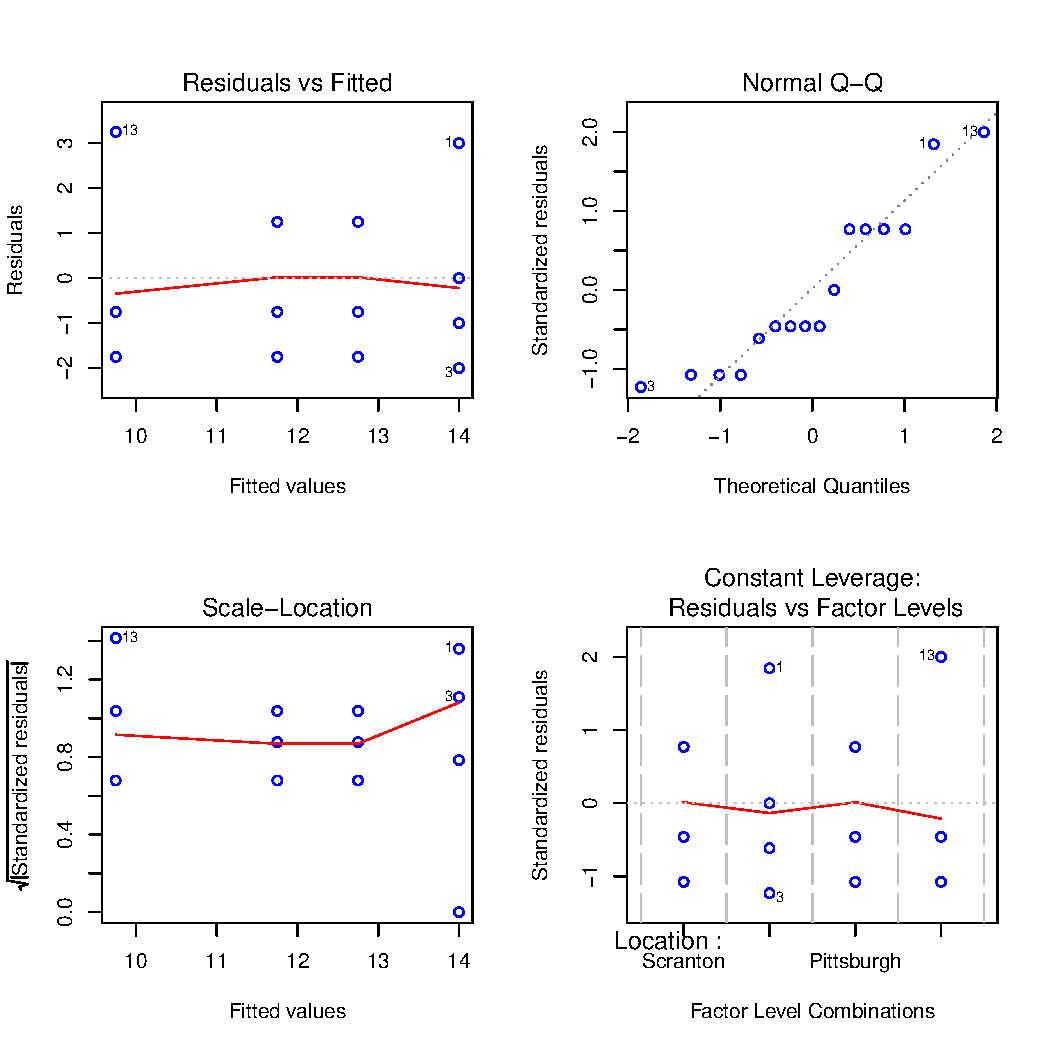
\includegraphics[width=7.5cm]{99_05_residAnovaPntWear1}
    \end{center}
\end{frame}

\begin{frame}[fragile]
  \vspace{0.25cm}
  Variance analysis:
  \begin{verbatim}
            Df Sum Sq Mean Sq F value p value  
Paint        3 30.688 10.2292  2.4428  0.1145
Residuals   12 50.250  4.1875     
  \end{verbatim}
\end{frame}

\begin{frame}
   Graphical check of the model:\\
  \vspace{.1cm}
  \begin{center}
    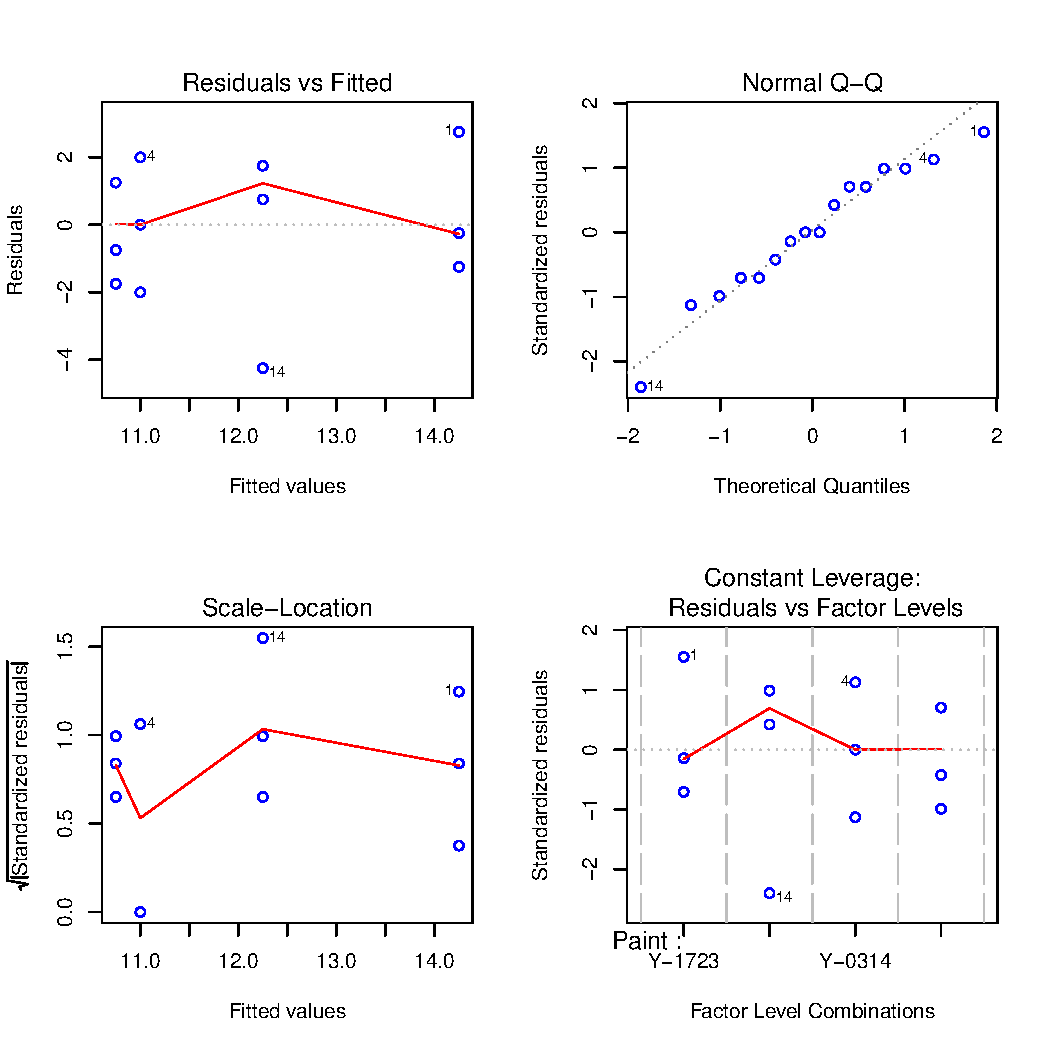
\includegraphics[width=7.5cm]{99_05_residAnovaPntWear2}
    \end{center}
\end{frame}

\begin{frame}[fragile]
  \vspace{0.25cm}
  Variance analysis:
  \begin{verbatim}
            Df Sum Sq Mean Sq F value  p value   
Paint        3 30.688 10.2292  7.9622 0.006685
Location     3 38.688 12.8958 10.0378 0.003133
Residuals    9 11.563  1.2847    
  \end{verbatim}
\end{frame}

\begin{frame}
   Graphical check of the model:\\
  \vspace{.1cm}
  \begin{center}
    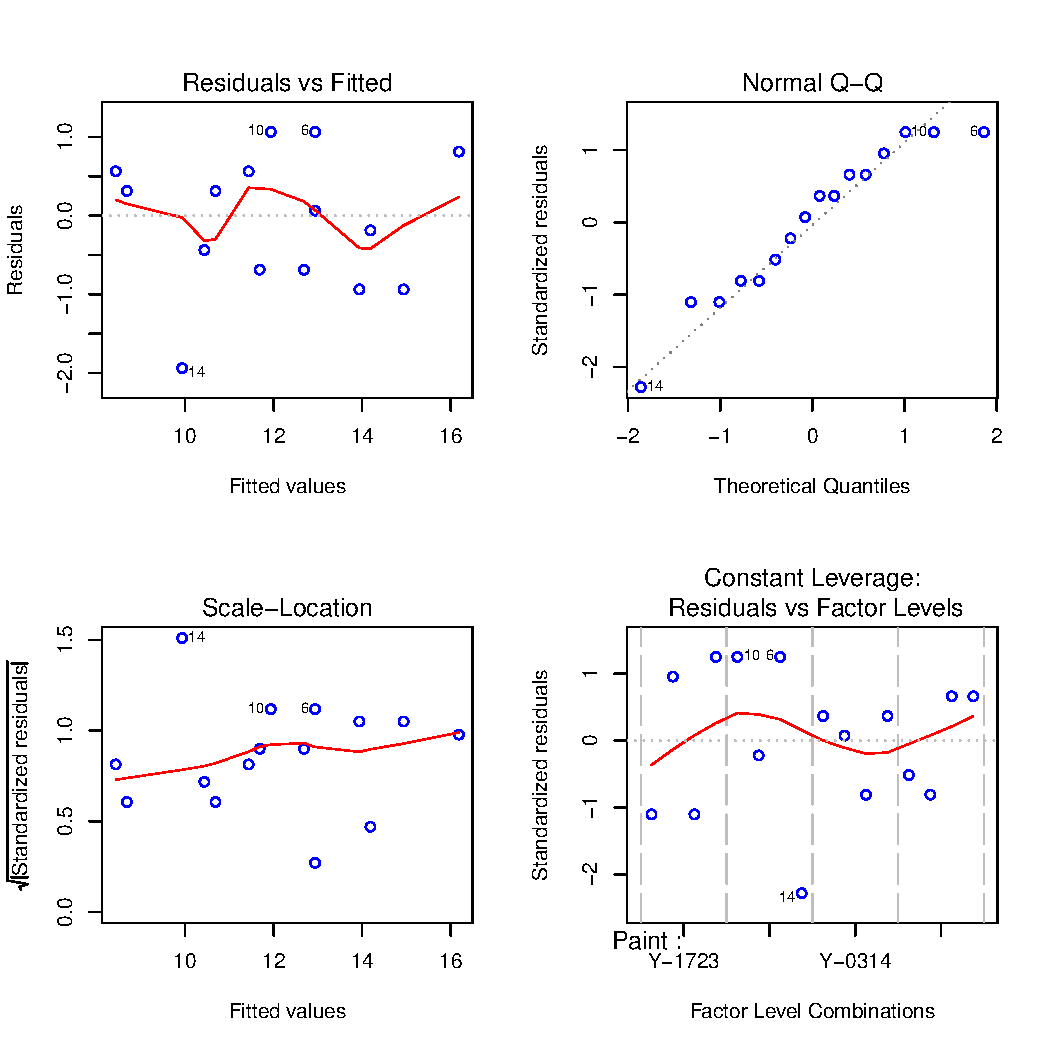
\includegraphics[width=7.5cm]{99_05_residAnovaPntWear3}
    \end{center}
\end{frame}



\livelloB{Penicillin production}

\begin{frame}
  \begin{description}
    \item[Data: ]penicillin.txt \\ 
    \item[Description: ]
      \begin{footnotesize}
        \begin{itemize}
          \item \textit{Mixture}: indicates the type of mixture chosen for the production (factor);
          \item \textit{Mode}: indicates the mode of production (factor);
          \item \textit{Penicillin}: indicates the quantity of penicillin produced.
        \end{itemize}
      \end{footnotesize}
    \item[Aims: ]
      \begin{footnotesize}
        The aim is to determine as the different modes of penicillin production (A, B, C, D) influence the quantity produced. Earlier It was observed that the mixture chosen for the production is rather variable and that this factor could somehow affect the production. So, It was decided to control also the effect of the mixture considering 5 mixtures (I, II, II, IV, V)  and using each of these in the four production processes. Let us note as in this case the interest is in the check if a difference of the effect on the quantities of penicillin produced with production mode exists, independently from the type of mixture used. 
      \end{footnotesize}
  \end{description}
\end{frame}

\begin{frame}
  \begin{description}
    \item[Aims: ]
      \begin{footnotesize}
        \begin{itemize}
          \item[-] Let us show the BW plot OF \textit{Penicillin} for each production mode and for each type of mixture.
          \item[-] By examining the BW plot, let us try to hypothesise if the modalities of production could detemine differences in the quantities of penicillin producted.
          \item[-] Performing an analysis of variance, let us check the hypothesis that the mode of production doesn't influence the quantity producted.
          \item[-] Let us look at what the differences may be due and let us repeat the analysis of variance considering the type of mixture.
        \end{itemize}
      \end{footnotesize}
  \end{description}
\end{frame}

\begin{frame}
  B-W Graph of \textit{Penicillin} for each mode of production:\\
  \vspace{-0.5cm}
  \begin{center}
    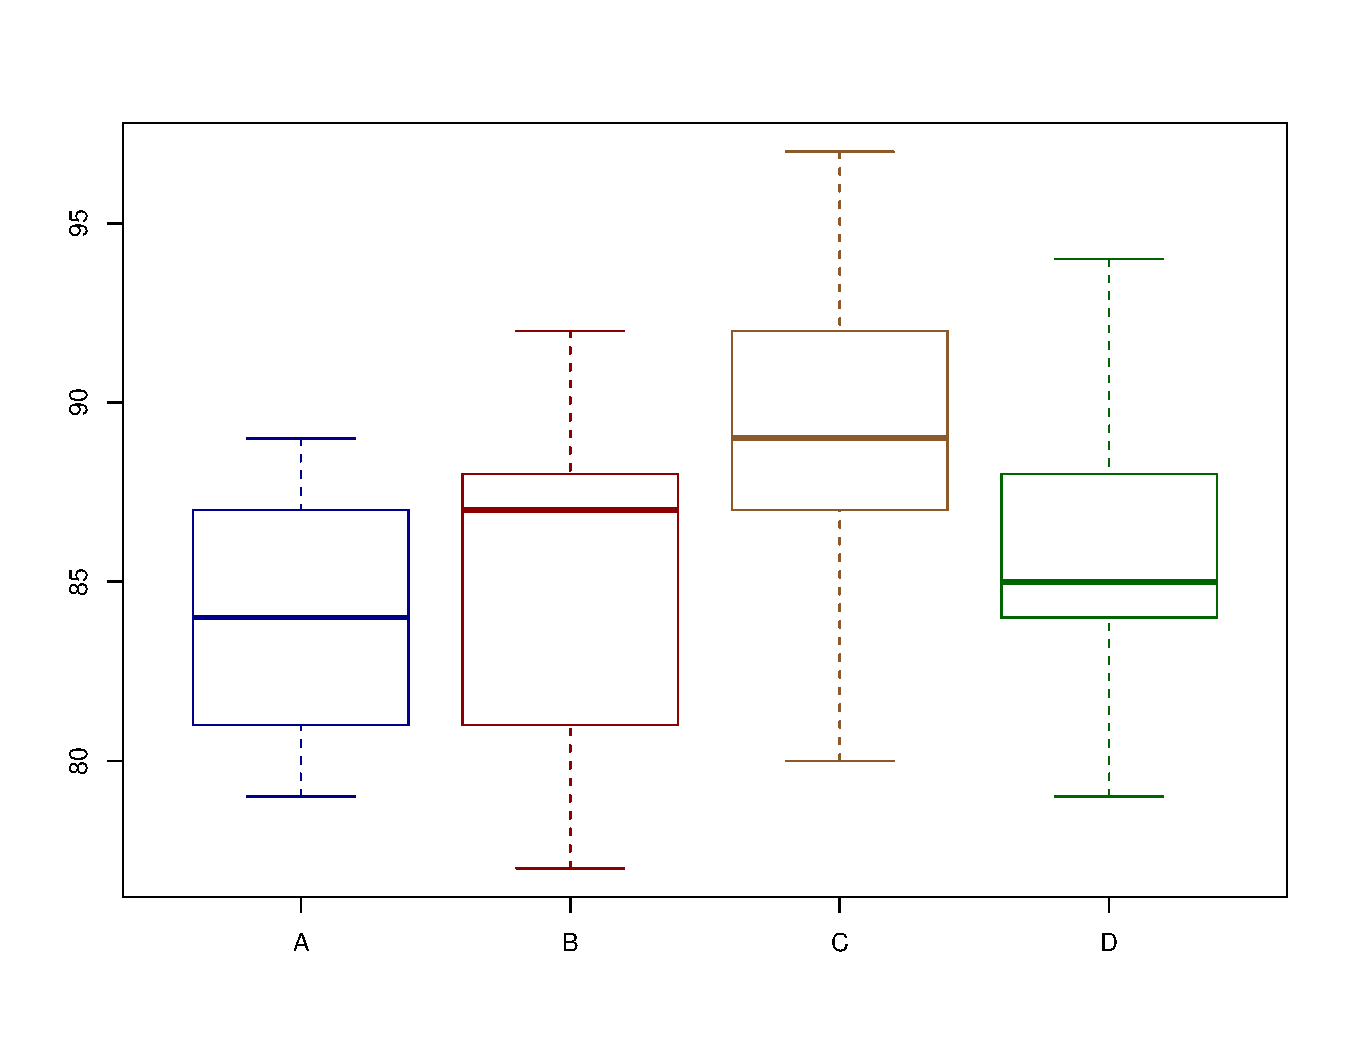
\includegraphics[width=11cm]{99_05_bwPenicillinMode.pdf}
  \end{center}
\end{frame}

\begin{frame}
  B-W Graph of \textit{Penicillin} for each type of mixture:\\
  \vspace{-0.5cm}
  \begin{center}
    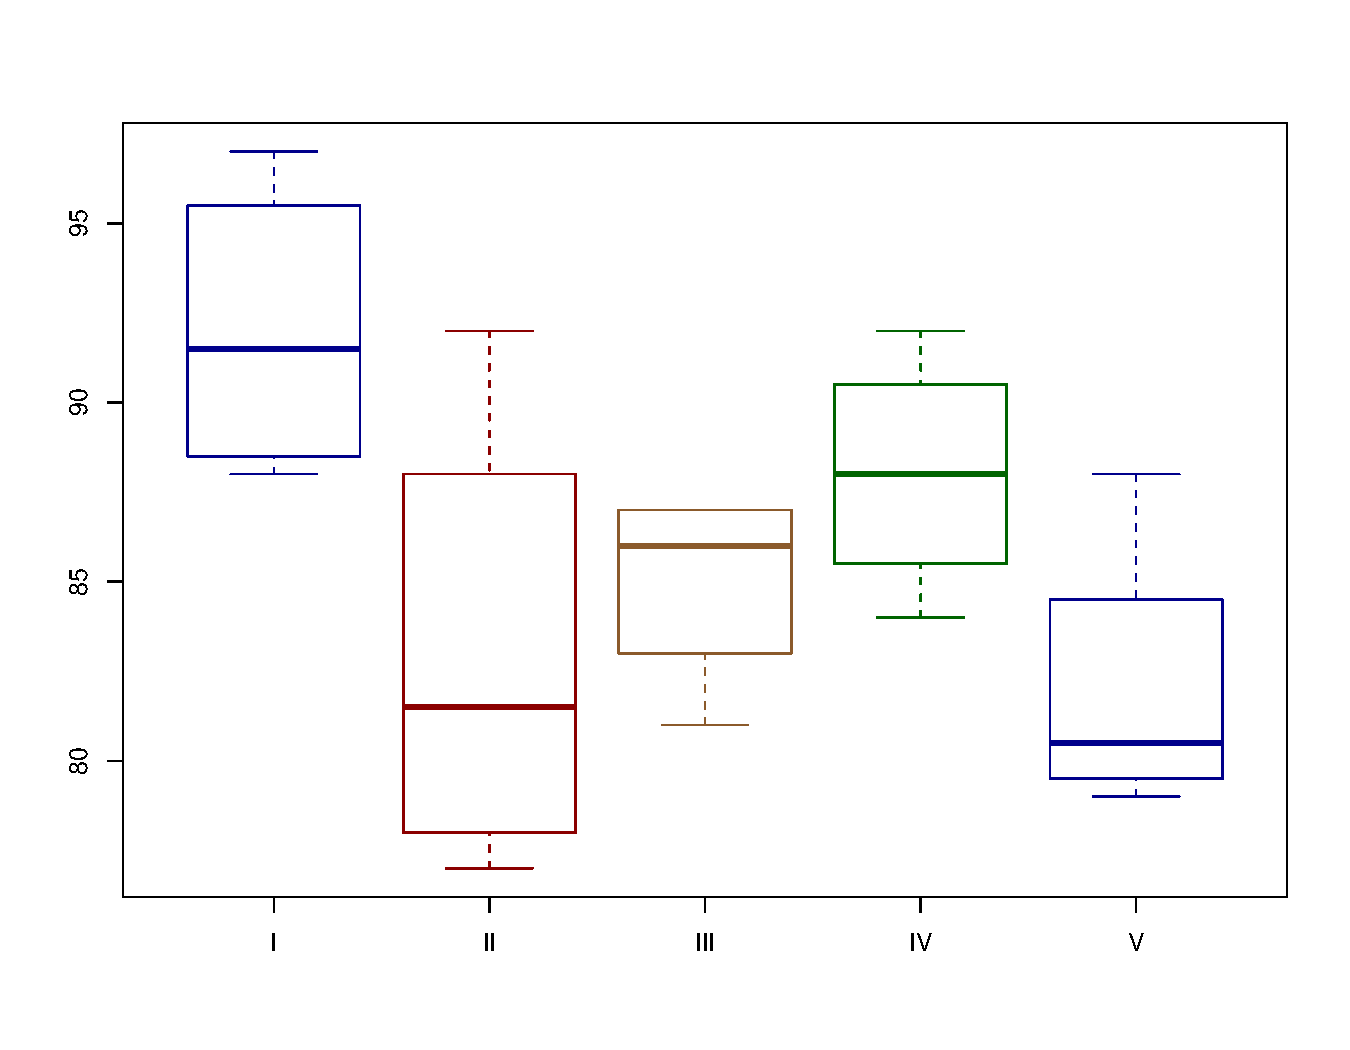
\includegraphics[width=11cm]{99_05_bwPenicillinMixture.pdf}
  \end{center}
\end{frame}

\begin{frame}
  Homoskedasticity of variances of \textit{Penicillin} for each mode of production\\
  \vspace*{0.25cm}
  Bartlett Test:\\
  \texttt{p value: 0.8755}\\
  \vspace*{0.25cm}
  Levene Test:\\
  \texttt{p value: 0.9388}\\
  \vspace*{0.75cm}
  Homoskedasticity of variances of \textit{Penicillin} for each type of mixture\\
  \vspace*{0.25cm}
  Bartlett Test:\\
  \texttt{p value: 0.6652}\\
  \vspace*{0.25cm}
  Levene Test:\\
  \texttt{p value: 0.5311}\\
\end{frame}

\begin{frame}[fragile]
  \vspace{0.25cm}
  Variance analysis (model that does not consider the type of mixture):
  \begin{verbatim}  
            Df Sum Sq Mean Sq F value p value
Mode         3     70  23.333  0.7619  0.5318
Residuals   16    490  30.625     
  \end{verbatim}
  \vspace{0.25cm}
  Variance analysis (model that consider the type of mixture):
  \begin{verbatim}  
            Df Sum Sq Mean Sq F value p value  
Mode         3     70  23.333  1.2389 0.33866  
Mixture      4    264  66.000  3.5044 0.04075
Residuals   12    226  18.833     
  \end{verbatim}
\end{frame}

\begin{frame}
   Graphical check of the model:\\
  \vspace{.1cm}
  \begin{center}
    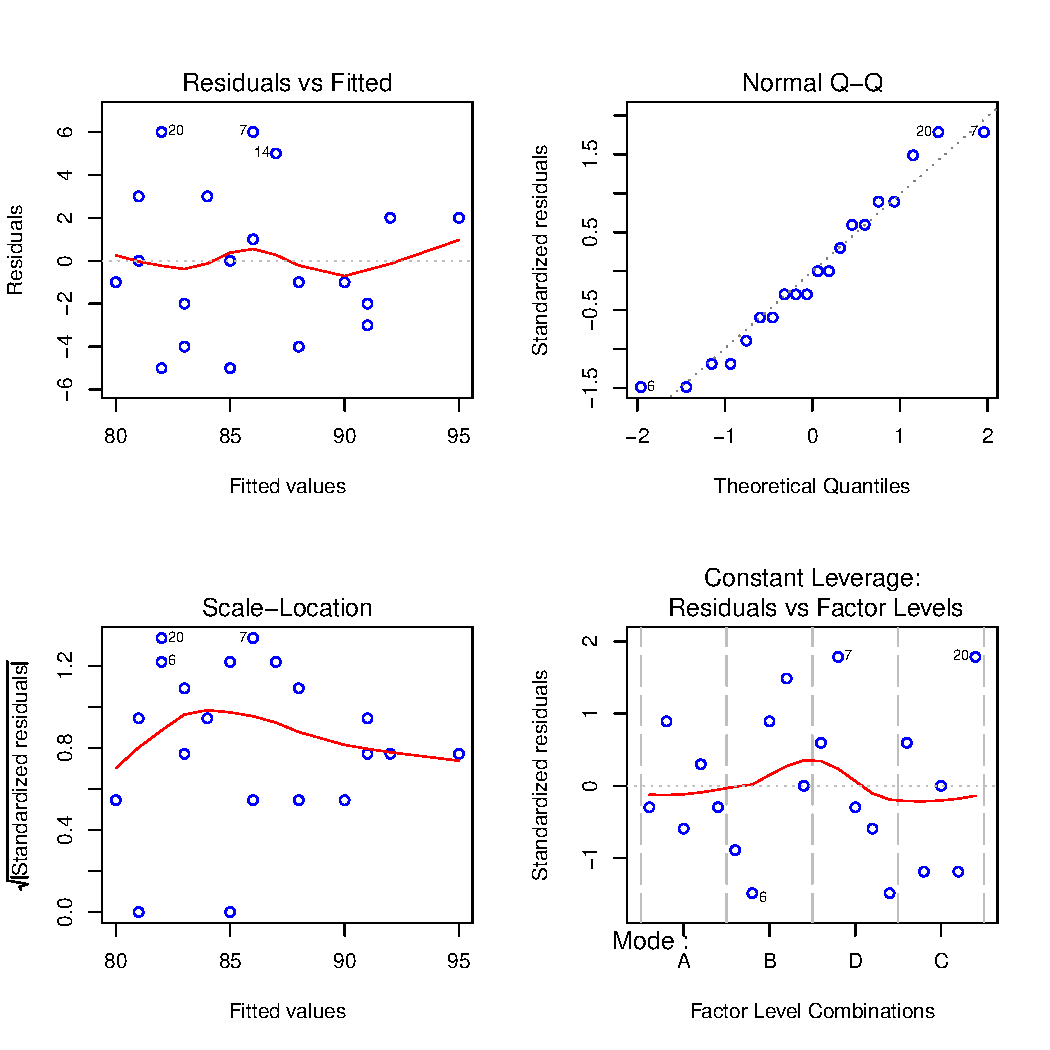
\includegraphics[width=7.5cm]{99_05_residAnovaPenicillin}
    \end{center}
\end{frame}


\livelloB{Effect of toxic agent}

\begin{frame}
  \begin{description}
    \item[Data: ]rats.txt \\ 
    \item[Description: ]
      \begin{footnotesize}
        \begin{itemize}
          \item \textit{Time}: identifies the survival time (in tens of hours);
          \item \textit{Poison}: identifies the poison type (factor);
          \item \textit{Treatment}: identifies the type of treatment (factor).
        \end{itemize}
      \end{footnotesize}
    \item[Aims: ]
      \begin{footnotesize}
        Let us consider three types of poison and four types of treatment. Each combination poison-treatment is administered to four rats. 
        \begin{itemize}
          \item[-] Let us show BW plot OF \textit{Time} for each type of poison.
          \item[-] Let us transform the variable \textit{Time} in its reciprocal.
          \item[-] Let us check the presence of the interaction effect between poison and type of treatment.
        \end{itemize}
      \end{footnotesize}
  \end{description}
\end{frame}

\begin{frame}
  B-W Graph of \textit{Time} separately for each type of poison:\\
  \vspace{-0.5cm}
  \begin{center}
    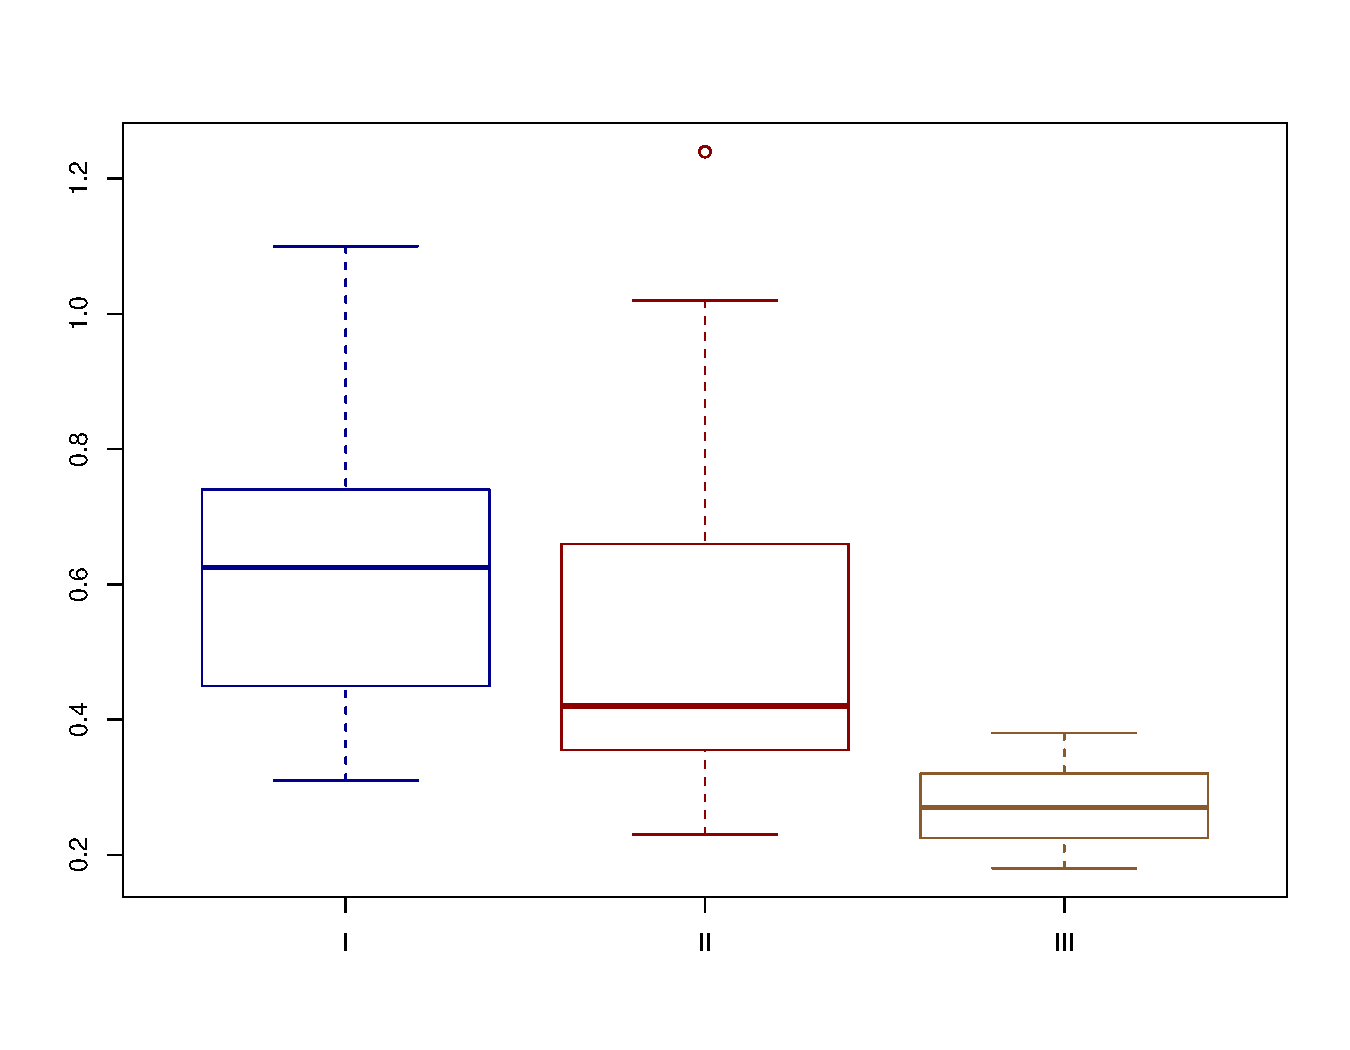
\includegraphics[width=11cm]{99_05_bwPoison.pdf}
  \end{center}
\end{frame}

\begin{frame}
  B-W Graph for the reciprocal of \textit{Time} for each type of poison:\\
  \vspace{-0.5cm}
  \begin{center}
    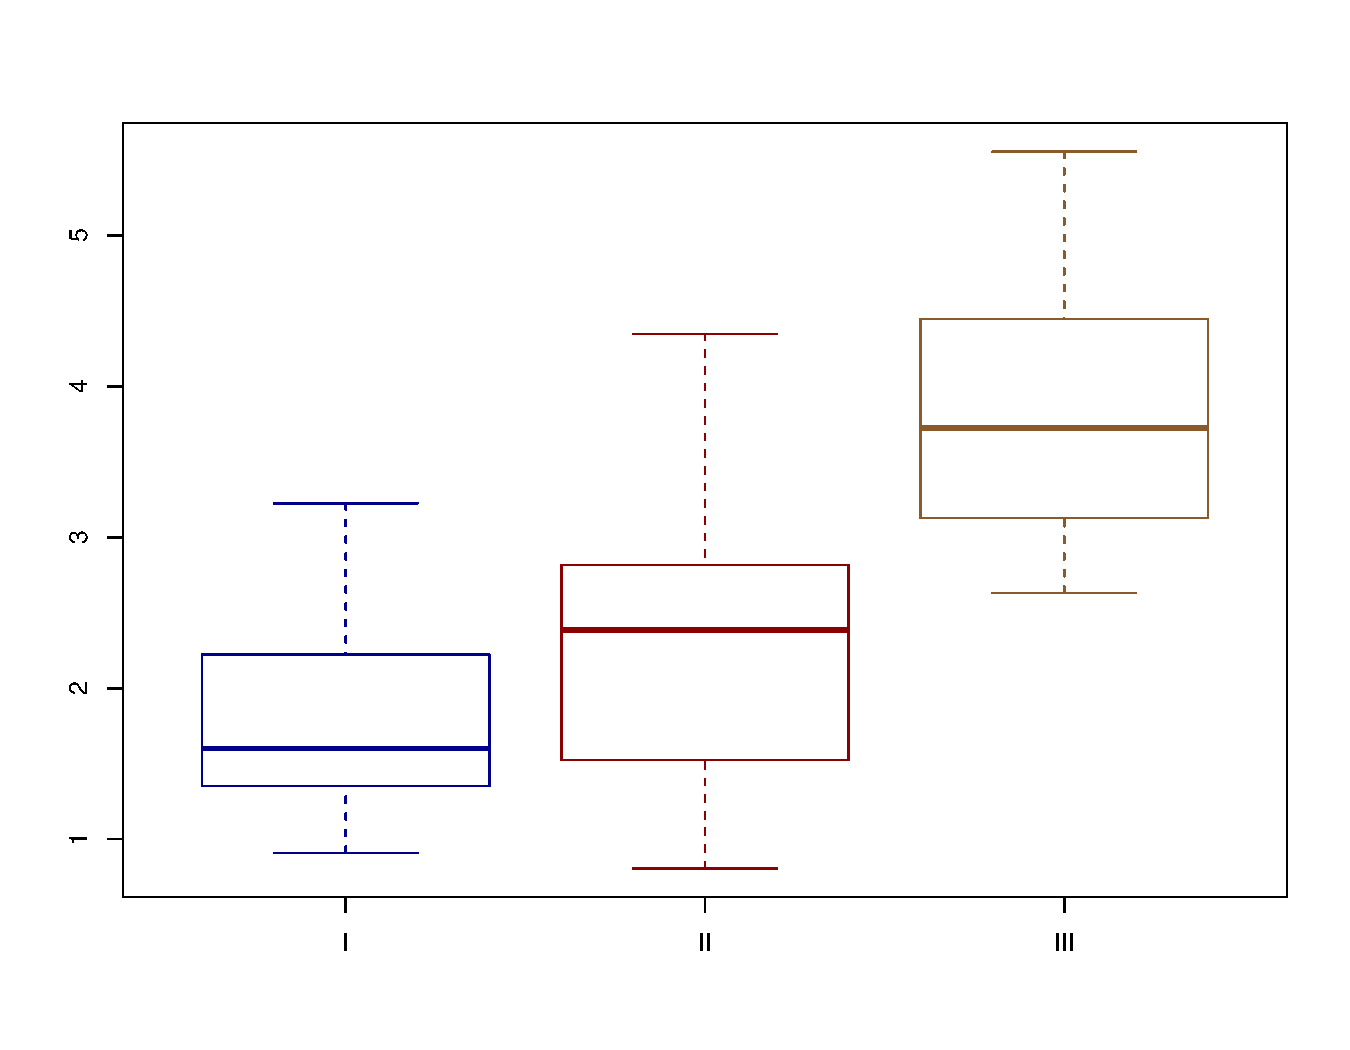
\includegraphics[width=11cm]{99_05_bwInvPoison.pdf}
  \end{center}
\end{frame}

\begin{frame}
  Normality\\
  \vspace*{0.25cm}
  Because of the low number of units within each groups, It is not possible to perform Anderson Darling test. However, analysing the B-W plot of the previous slide, the normality assumption is considered valid. \\
  \vspace{1cm}
  Homoskedasticity of variances of the reciprocal of \textit{Time} for each type of poison\\
  \vspace*{0.25cm}
  Bartlett Test:\\
  \texttt{p value: 0.2105}\\
  \vspace*{0.75cm}
  Levene Test:\\
  \texttt{p value: 0.1915}\\
\end{frame}

\begin{frame}[fragile]
  \vspace{0.25cm}
  Variance analysis (model with interaction):
  \begin{verbatim}  
                 Df Sum Sq Mean Sq F value   p value   
Treatment         3 20.414  6.8048 28.3431 1.376e-09
Poison            2 34.877 17.4386 72.6347 2.310e-13
Treatment:Poison  6  1.571  0.2618  1.0904    0.3867    
Residuals        36  8.643  0.2401      
  \end{verbatim}
  \vspace{0.25cm}
  Variance analysis (model without interaction):
  \begin{verbatim}  
            Df Sum Sq Mean Sq F value   p value    
Treatment    3 20.414  6.8048  27.982 4.192e-10
Poison       2 34.877 17.4386  71.708 2.865e-14
Residuals   42 10.214  0.2432      
  \end{verbatim}
\end{frame}

\begin{frame}
   Graphical check of the model:\\
  \vspace{.1cm}
  \begin{center}
    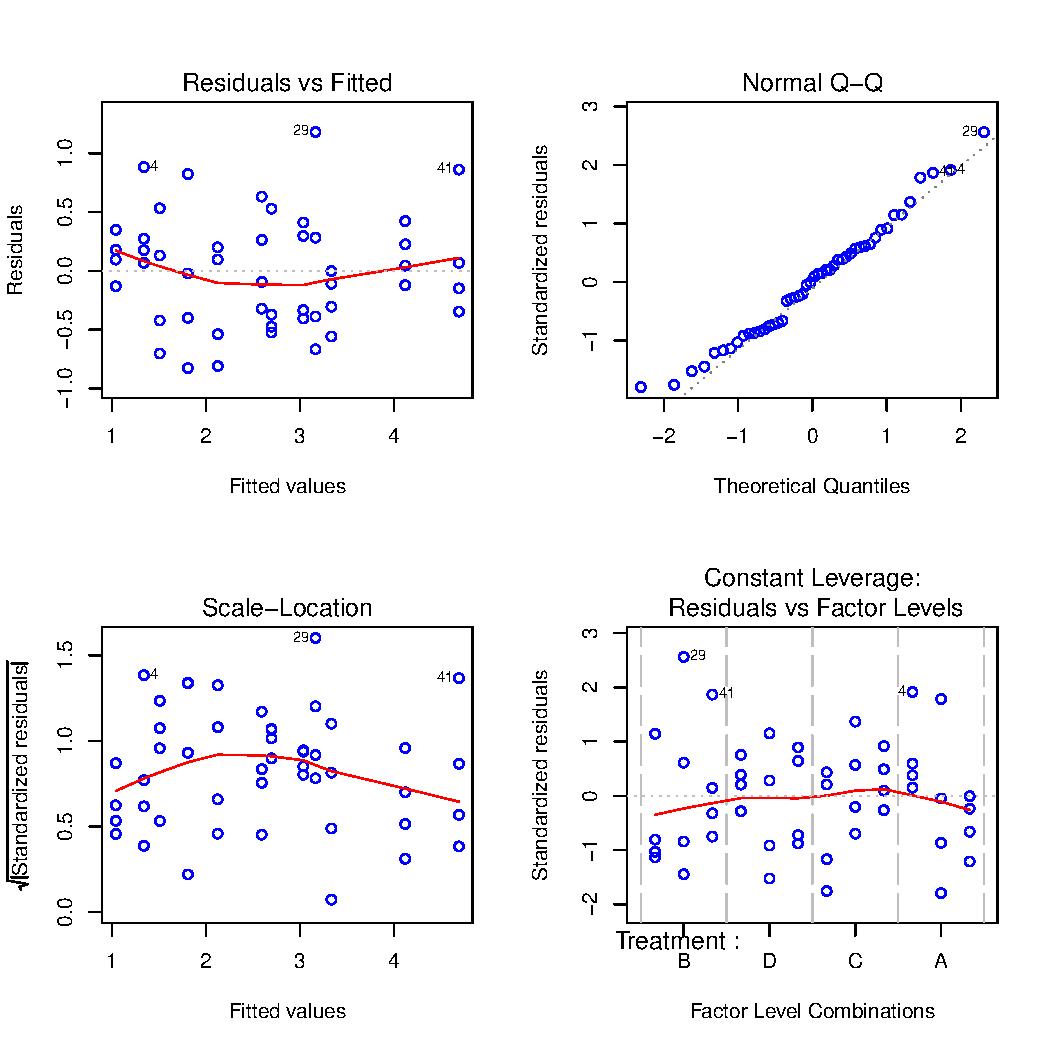
\includegraphics[width=7.5cm]{99_05_residAnovaInvTreatmentPoison}
    \end{center}
\end{frame}

\livelloB{Solvent for varnish}

\begin{frame}
  \begin{description}
    \item[Data: ]varnish.txt \\ 
    \item[Description: ]
      \begin{footnotesize}
        \begin{itemize}
          \item \textit{Solvent}: indicates the type of solvent (factor);
          \item \textit{Varnish}: indicates the type of varnish (factor);
          \item \textit{Time}: indicates the time necessary to dissolve the stain (minutes).
        \end{itemize}
      \end{footnotesize}
    \item[Aims: ]
      \begin{footnotesize}
        The aim is to evaluate the efficacy of a solvent to dissolve stains of nail varnish from fabrics. It is used two types of solvent and three types of varnish. The experiment consists of immersing 5 stained fabrics by a certain type of varnish into a bowl with a solvent, measuring the time (in minutes) necessary to dissolve the stain. 
        \begin{itemize}
          \item[-] Let us evaluate also if there are differences in the types of solvent in respect of the types varnish that produced the stain.
        \end{itemize}
      \end{footnotesize}
  \end{description}
\end{frame}

\begin{frame}
  B-W Graph of \textit{Time} separately for each type of solvent:\\
  \vspace{-0.5cm}
  \begin{center}
    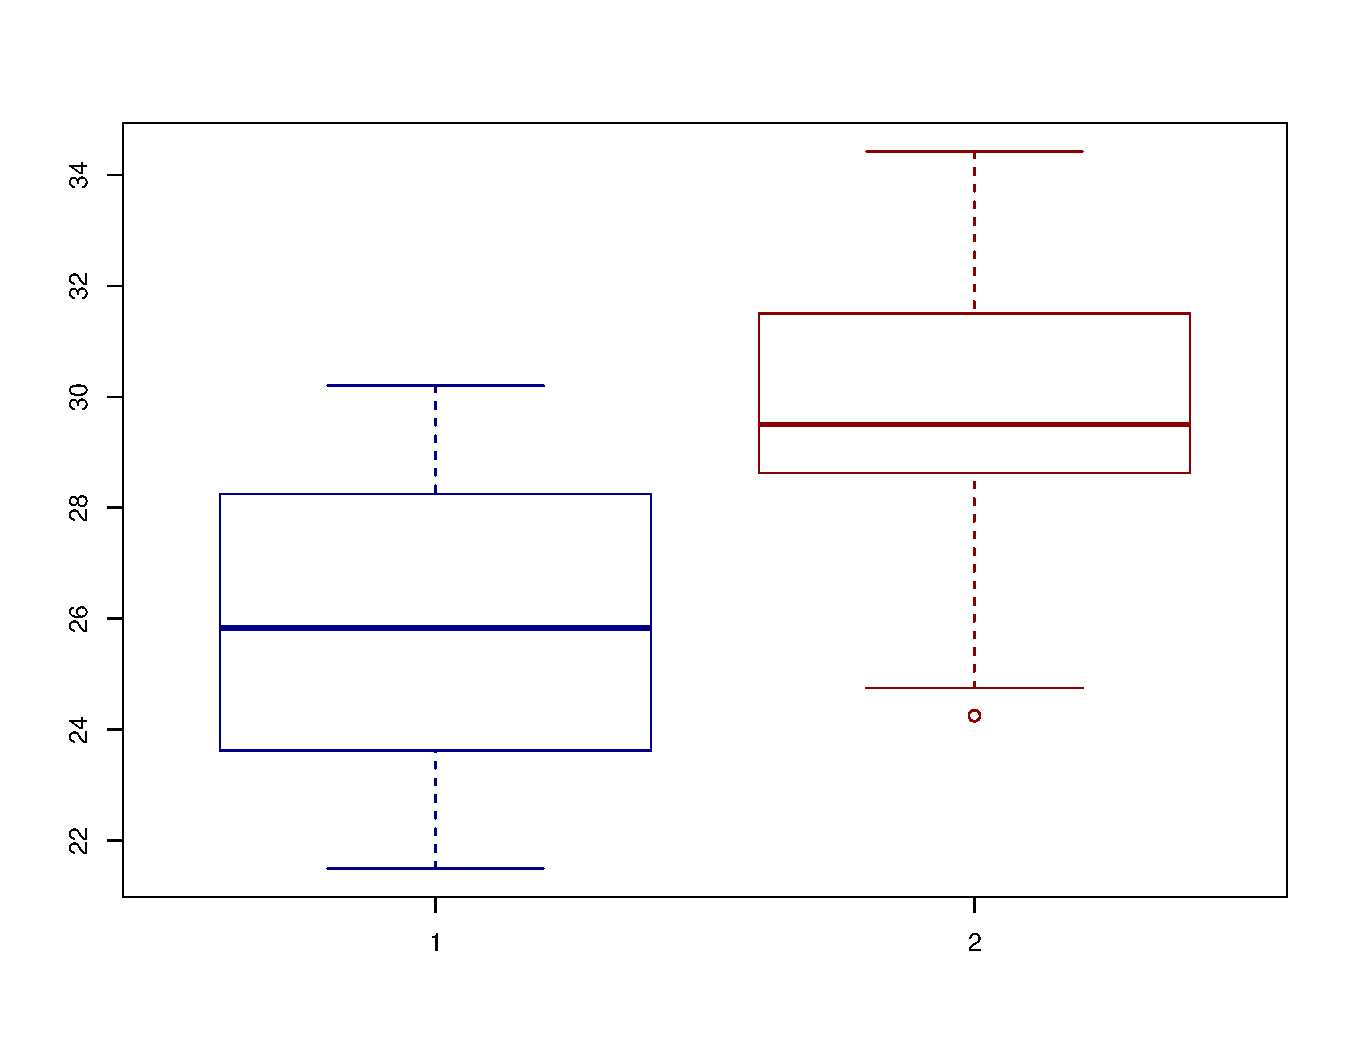
\includegraphics[width=11cm]{99_05_bwVarnishSolvent.pdf}
  \end{center}
\end{frame}

\begin{frame}
  B-W Graph of the reciprocal of \textit{Time} for each type of varnish:\\
  \vspace{-0.5cm}
  \begin{center}
    \includegraphics[width=11cm]{99_05_bwVarnishVarnish.pdf}
  \end{center}
\end{frame}

\begin{frame}
  Normality\\
  \vspace*{0.25cm}
  Anderson-Darling test doesn't reject the hypothesis of normality of \textit{Time} separately for each type of solvent and of \textit{Time} separately for each type of varnish.\\
  \vspace{1cm}
  Homoskedasticity of variances\\
  \vspace*{0.25cm}
  Both levene and Bartlett test doesn't reject the hypothesis of the homoskedasticity of \textit{Time}separately for each type of solvent and of \textit{Time}separately for each type of varnish.\\    
\end{frame}

\begin{frame}[fragile]
  \vspace{0.25cm}
  Variance analysis (complete model):
  \begin{verbatim}  
                Df  Sum Sq Mean Sq F value  p value   
Varnish          2  18.636   9.318  1.0695 0.358990   
Solvent          1  97.416  97.416 11.1810 0.002706
Varnish:Solvent  2   7.673   3.836  0.4403 0.648930   
Residuals       24 209.104   8.713  
  \end{verbatim}
  \vspace{0.25cm}
  Variance analysis (model which considers only the type of solvent):
  \begin{verbatim}  
            Df  Sum Sq Mean Sq F value  p value
Solvent      1  97.416  97.416  11.587 0.002022
Residuals   28 235.412   8.408      
  \end{verbatim}
\end{frame}

\begin{frame}
   Graphical check of the model:\\
  \vspace{.1cm}
  \begin{center}
    \includegraphics[width=7.5cm]{99_05_residAnovaVarnish}
    \end{center}
\end{frame}

\livelloA{Simple regression}

\livelloB{Impurities in paints}

\begin{frame}
  \begin{description}
    \item[Data: ]paint.txt \\ 
    \item[Description: ]
      \begin{footnotesize}
        \begin{itemize}
          \item \textit{Stirrate}: identifies the rate of agitation (revolution) applied to the container (rpm, revolutions per minute);
          \item \textit{Impurity}: indentifies the number of impurities (lumps) present in the containers of paint.
        \end{itemize}
      \end{footnotesize}
    \item[Aims: ]
      \begin{footnotesize}
        The number of impurities (lumps) present in the containers of paint depends on the rate of agitation applied to the container. The aim is to determine the relation between the rate of agitation (revolution) and the number of lumps.
        \begin{itemize}
          \item[-] Let us compute the main descriptive statistics of \textit{Impurity}.
          \item[-] Let us compute the correlation between \textit{Impurity} and \textit{Stirrate}.
          \item[-] Let us graphically represent the relation between these variables.
          \item[-] Let us compute a simple linear regression between \textit{Stirrate} and \textit{Impurity}.
          \item[-] Does \textit{Stirrate} influence \textit{Impurity}? How?
          \item[-] How many variability is explained by the regression? Which is the residual variability?  
        \end{itemize}
      \end{footnotesize}
  \end{description}
\end{frame}

\begin{frame}
  Computation of descriptive statistics and B-W graphic of \textit{Impurity}:\\
  \vspace{.3cm}
  \begin{scriptsize}
    \begin{center}
      \begin{tabular}{|c|cccccc|c|}
        \hline
        \textbf{n} & \textbf{Min.} & \textbf{1st. Qu.} & \textbf{Median} & \textbf{Mean} & \textbf{3rd. Qu.} & \textbf{Max.} & \textbf{Sd}\\
        \hline
        12 & 8.40 & 11.45 & 14.00 & 13.87 & 16.42 & 18.90 & 3.4076\\
        \hline	
      \end{tabular}
    \end{center}
    \vspace{0.3cm}
    \begin{center}
      \includegraphics[width=6cm]{99_06_bwImpurity}
    \end{center}
  \end{scriptsize}
\end{frame}

\begin{frame}
  Scatterplot matrix of the relation between correlation and significativity: \\
  \begin{center}
    \includegraphics[width=5.5cm]{99_06_splmatImpurity}
  \end{center}
\end{frame}

\begin{frame}
  Scatterplot of the relation with the regression line:\\
  \vspace{.3cm}
  \begin{center}
    \includegraphics[width=7.5cm]{99_06_regrStirrateImpurity}
  \end{center}
\end{frame}

\begin{frame}[fragile]
  Regression analysis:\\
  \begin{small}
    \begin{verbatim}
Coefficients:
               Estimate  Std. Error  t value   p value    
(Intercept)    -0.28928     1.22079   -0.237     0.817
Stirrate        0.45664     0.03844   11.880  3.21e-07

Residual standard error: 0.9193 on 10 degrees of freedom
Multiple R-squared: 0.9338,	Adjusted R-squared: 0.9272 
F-statistic: 141.1 on 1 and 10 DF,  p-value: 3.211e-07
    \end{verbatim}
  \end{small}
  Anderson-Darling test:\\
  \begin{small}
    \begin{verbatim}
A = 0.4329, p-value = 0.2515
    \end{verbatim}
  \end{small}
\end{frame}

\begin{frame}
  Graphical check of the regression model:\\
  \vspace{.1cm}
  \begin{center}
    \includegraphics[width=7.5cm]{99_06_residStirrateImpurity}
    \end{center}
\end{frame}

\begin{frame}
  \begin{small}
    \begin{itemize}
      \item The relation that ``links'' the revolution rate seems to be well described by a simple linea regression, at least for the considered interval of \textit{Stirrate}.  
      \item The estimated formula is the follows: $ Impurity = -0.2893 + 0.4566 \cdot Stirrate $.
      \item The p-value for the significativity of the coefficient of \textit{Stirrate} is extremely low. This fact confirms the ``non random'' existing relation between the two variables.  
      \item $ R^2 $ value is equal to 0.9338; this fact confirms that the model explais well the observed data.
      \item The standard deviation of the residual is 0.9193.
      \item The p-value of the intercept estimate is 0.817. This would indicate an intercept potentially equal to 0. 
      \item Keeping the intercept value equal to the estimate,  with value of \textit{Stirrate}=0, the mean number of imputities would be negative: the results of the regression couldn't be ``extended'' too outside experimental field. 
    \end{itemize}
  \end{small}
\end{frame}

\livelloB{Resistance of a polypropylene film}

\begin{frame}
  \begin{description}
    \item[Data: ]temperatures.txt \\ 
    %\item[Origine dati: ]http://www.weibull.com/DOEWeb/simple_linear_regression_analysis.htm\\
    \item[Description: ]
      \begin{footnotesize}
        \begin{itemize}
          \item \textit{Yield}: indicates the resistance of a polypropylene film;
          \item \textit{Temperature}: indicates the temperature of a chemical process.
        \end{itemize}
      \end{footnotesize}
    \item[Aims: ]
      \begin{footnotesize}
        The resistance of a polypropylene film depends on the temperature on which the chemical process is performed. The aim is to determine the relation between resistance and temperature.
        \begin{itemize}
          \item[-] Let us graphically represent the relation between the two variables.
          \item[-] Let us compute a simple linear regression between \textit{Yield} and \textit{Temperature}.
          \item[-] Does \textit{Yield} influences \textit{Temperature}? How?
          \item[-] How many variability is explained by the regression? Which is the residual variability?    
        \end{itemize}
      \end{footnotesize}
  \end{description}
\end{frame}

\begin{frame}
%   \begin{small}
    \begin{itemize}
      \item The relation  that ``links'' the revolution rate with the number of impurities seems to be well described by a simple linear regression, at least in the considered interval of \textit{Stirrate}. 
      \item The estimated formula is the follows: $ Yield = 17.00 + 2.00 \cdot Temperature $.
      \item The p-value for the significativity of the coefficient of \textit{Temperature} is extremely low. This fact confirms the ``non random'' existing relation between the two variables.
      \item $ R^2 $ value is 0.9831. This fact confirms that the model explains well the observed data.
    \end{itemize}
%   \end{small}
\end{frame}

\begin{frame}
  \begin{description}
    \item[Data: ]production.txt \\ 
    %\item[Origine dati: ]http://www.stat.tamu.edu/~sheather/book/docs/datasets/production.txt\\
    \item[Description: ]
      \begin{footnotesize}
        \begin{itemize}
          \item \textit{RunSize}: indicates the number of pieces produced in a productive process;
          \item \textit{RunTime}: indicates the duration of a productive process.
        \end{itemize}
      \end{footnotesize}
    \item[Aims: ]
      \begin{footnotesize}
        The duration of a productive process depends on the number of pieces produced.
        \begin{itemize}
          \item[-] Let us graphically represent the relation between the two variables.
          \item[-] Let us compute a simple linear regression between \textit{RunTime} a \textit{RunSize}.
          \item[-] Does \textit{RunSize} influences \textit{RunTime}? How?
          \item[-] How many variability is explained by the regression? Which is the residual variability? 
        \end{itemize}
      \end{footnotesize}
  \end{description}
\end{frame}

\begin{frame}
%   \begin{small}
    \begin{itemize}
      \item The relation that ``links'' the duration of the productiove process with the number of pieces produced seems to be well descibed by a simple linear regression.
      \item The esimated formula is the follows:  $ RunTime = 149.75 + 0.26 \cdot RunSize $.
      \item The p-value for the significativity of the coefficient of \textit{RunSize} is extremely low. This fact confirms the ``non random'' existing relation between the two variables.
      \item $ R^2 $ value is 0.7302. This fact confirms that the model explains well the observed data.
    \end{itemize}
%   \end{small}
\end{frame}


\livelloA{Polynomial regression}

\livelloB{Pressure Switch}

\begin{frame}
  \begin{description}
    \item[Data: ]switch.txt \\ 
    \item[Description: ]
      \begin{footnotesize}
        \begin{itemize}
	  \item \textit{BuildOrder}: indicates the order in which the switches have been assembled;
          \item \textit{RunOrder}: indicates the order in which the observations have been collected;
          \item \textit{DThickness}: indicates the thickness of the diaphragm (mm);
          \item \textit{SetPoint}: indicates the pressure at which the switch opens (KPa).
        \end{itemize}
      \end{footnotesize}
    \item[Aims: ]
      \begin{footnotesize}
        A pressure switch has a membrane whose thickness (in mm) influences the pressure required to trigger the switch itself. The aim is to determine the thickness of the membrane for which the switch ``trig'' with a pressure equal to $165 \pm 15$ KPa. 25 switches with different thickness of the membrane was analysed. 
        \begin{itemize}
          \item[-] Let us compute the descriptive statistics of the variable \textit{SetPoint}.
          \item[-] Let us graphically represent the relation \textit{DThickness}-\textit{SetPoint}.
          \item[-] Let us compute a linear regression between the two variables.
          \item[-] Does \textit{DThickness} influences \textit{SetPoint}? Is the model correct?
          %\item[-] Si determini lo spessore della membrana per cui l'interruttore ``scatta'' con una pressione pari a $165 \pm 15$ KPa.
          \item[-] How can be modified the model? Which are the final characteristics?
        \end{itemize}
      \end{footnotesize}
  \end{description}
\end{frame}

\begin{frame}
  Computation of the descriptive statistics and of the B-W Graphic of \textit{SetPoint}:\\
  \vspace{.3cm}
  \begin{scriptsize}
    \begin{center}
      \begin{tabular}{|c|cccccc|c|}
        \hline
        \textbf{n} & \textbf{Min.} & \textbf{1st. Qu.} & \textbf{Median} & \textbf{Mean} & \textbf{3rd. Qu.} & \textbf{Max.} & \textbf{Sd}\\
        \hline
        25 & 144.7 & 157.4 & 174.8 & 181.1 & 200.0 & 231.7 & 27.70 \\
        \hline	
      \end{tabular}
    \end{center}
    \vspace{0.3cm}
    \begin{center}
      \includegraphics[width=6cm]{99_06_bwSetPoint}
    \end{center}
  \end{scriptsize}
\end{frame}

\begin{frame}
  Scatterplot of the relation with regression line:\\
  \vspace{.3cm}
  \begin{center}
    \includegraphics[width=7.5cm]{99_06_regrDThicknessSetPoint}
  \end{center}
\end{frame}

\begin{frame}[fragile]
  Regression analysis:\\
  \begin{small}
    \begin{verbatim}
Coefficients:
               Estimate Std. Error t value  p value    
(Intercept)      51.145      7.266   7.039 3.58e-07
DThickness      185.637     10.174  18.246 3.54e-15

Residual standard error: 7.194 on 23 degrees of freedom
Multiple R-squared: 0.9354,	Adjusted R-squared: 0.9326 
F-statistic: 332.9 on 1 and 23 DF,  p-value: 3.542e-15
    \end{verbatim}
  \end{small}
  Anderson-Darling test:\\
  \begin{small}
    \begin{verbatim}
A = 0.1865, p-value = 0.8949
    \end{verbatim}
  \end{small}
\end{frame}

\begin{frame}
  Regression line with confidence and prediction intervals at 95\% level:\\  
  \vspace{.3cm}
  \begin{center}
    \includegraphics[width=6.5cm]{99_06_regrIntDThicknessSetPoint}
  \end{center}
\end{frame}

\begin{frame}
  Graphical check of the regression model:\\
  \vspace{.1cm}
  \begin{center}
    \includegraphics[width=7.5cm]{99_06_residDThicknessSetPoint}
    \end{center}
\end{frame}

\begin{frame}
  \begin{small}
    \begin{itemize}
      \item The relation that ``links'' the thickness of diaphragm with the pressure for which the switch trigs seems well described by a simple linear regression,  at least in the considered interval.
      \item The estimated formula is the follows: $ SetPoint = 51.145 + 185.637 \cdot DThickness $.
      \item The p-value for the significativity of the coefficient of \textit{DThickness} is extremely low. This fact confirms the  ``non random'' existing relation between the two variables.
      \item $ R^2 $ value is 0.9354. This fact confirms that the model explains well the observed data.
      \item The p-value of the estimate of the intercept is very low. The intercept is significative.
      \item The graphic of the residual values in respect of the estimated values shows a curvilinear trend. This fact implies that the model could be improved, for example with a quadratic model.
    \end{itemize}
  \end{small}
\end{frame}

\begin{frame}
  Scatterplot of the relation with polynomial regression curve:\\
  \vspace{.3cm}
  \begin{center}
    \includegraphics[width=6.5cm]{99_06_regrPolDThicknessSetPoint}
  \end{center}
\end{frame}

\begin{frame}[fragile]
  Polynomial regression analysis:\\
  \begin{small}
    \begin{verbatim}
Coefficients:
              Estimate Std. Error t value  p value
(Intercept)     202.47      26.24   7.717 1.07e-07
DThickness     -265.10      77.19  -3.434  0.00237
DThickness^2    321.96      54.94   5.860 6.76e-06

Residual standard error: 4.597 on 22 degrees of freedom
Multiple R-squared: 0.9748,	Adjusted R-squared: 0.9725 
F-statistic: 424.9 on 2 and 22 DF,  p-value: < 2.2e-16 
    \end{verbatim}
  \end{small}
  Anderson-Darling test:\\
  \begin{small}
    \begin{verbatim}
A = 0.4204, p-value = 0.3005
    \end{verbatim}
  \end{small}
\end{frame}

\begin{frame}
  Polynomial regression curve with a confidence and prediction interval at 95\% level:\\
  \vspace{.3cm}
  \begin{center}
    \includegraphics[width=6.5cm]{99_06_regrPolIntDThicknessSetPoint}
  \end{center}
\end{frame}

\begin{frame}
  \begin{small}
    \begin{itemize}
      \item The p-value of the quadratic term is significant, so the quadratic term explains a great quantity of variation in the response in respect of that explained by the linear model.
      \item The estimated formula is the follows: $ SetPoint = 202.47 - 265.10 \cdot DThickness + 321.96 \cdot DThickness^2 $.
      \item $ R^2 $ value is 0.9748, This value is certainly better than the same value of the simple linear model. 
      \item $ R^2 $ can never decrease. It will be always higher with the addiction of  predictors, even if the predictors addicted don't improve the model. 
      \item The value of the adjusted  $ R^2 $ allows one to compare models with different number of parameters.
      \item The value of the adjusted  $ R^2 $ of the polynomial model (0.9725) is greater than the same value of the simple linear model (0.9326).
    \end{itemize}
  \end{small}
\end{frame}

\begin{frame}
  Graphical check of the polynomial regression model:\\
  \vspace{.1cm}
  \begin{center}
    \includegraphics[width=7.5cm]{99_06_residPolDThicknessSetPoint}
    \end{center}
\end{frame}

\begin{frame}
  \vspace{0.75cm}
  \begin{itemize}
    \item The graphic of the estimated values vs residuals doesn't show any systematic trend of the residuals and the variance seems to be the same for each estimated value.
    \vspace{0.5cm}
    \item The residuals are quite well aligned on the line representing the quantile of the normal distribution: It is reasonable to assume that they are then normally distributed.
  \end{itemize}
\end{frame}

\begin{frame}
  \begin{floatingfigure}[l]{7cm}
    \vspace{-1cm}
    \centering
    \includegraphics[width=7.5cm]{99_06_regrPol165DThicknessSetPoint}\\
  \end{floatingfigure}
  \begin{footnotesize}
    \vspace{1cm}
    Using the quadratic regression model, the best choice for the thickness of diaphragm is approximately 0.64 mm. This result is obtained replacing 165 for \textit{SetPoint} (y) in the regression model and solving the thickness (\textit{DThickness} (x) using a quadratic equation.
  \end{footnotesize}
\end{frame}

\livelloB{Antierosion screens}

\begin{frame}
  \begin{description}
    \item[Data: ]erosion.txt \\ 
    \item[Description: ]
      \begin{footnotesize}
        \begin{itemize}
	  \item \textit{Hardness}: indicates the hardness of the turbine;
          \item \textit{Abrasion}: indicates the abrasion.
        \end{itemize}
      \end{footnotesize}
    \item[Aims: ]
      \begin{footnotesize}
        A builder of turbines wants to know how an antierosion screen is able to resist the abrasive action during use. The direct measurement of abrasion is difficult, expensive and destructive. However, the builder hopes to produce an abrasion resistance using the hardness of the steel. The loss due to abrasion and the hardness were measured on 24 antierosion screens, chosen randomly.   
        \begin{itemize}
          \item[-] Let us graphically represent the relation between the variables.
          \item[-] Let us compute a simple linear regression between the variables.
          \item[-] Let us try to introduce the terms of second and third degree in the model.
        \end{itemize}
      \end{footnotesize}
  \end{description}
\end{frame}

\begin{frame}
  Scatterplot:\\
  \vspace{.3cm}
  \begin{center}
    \includegraphics[width=7.5cm]{99_06_scattHardnessAbrasion}
  \end{center}
\end{frame}

\begin{frame}
  Regression line:\\
  \vspace{.3cm}
  \begin{center}
    \includegraphics[width=7.5cm]{99_06_regrIntHardnessAbrasion}
  \end{center}
\end{frame}

\begin{frame}[fragile]
  Regression analysis:\\
  \begin{small}
    \begin{verbatim}
Coefficients:
             Estimate Std. Error t value  p value   
(Intercept) 2671.0980   279.0055   9.574 2.65e-09
x             -3.1292     0.3991  -7.841 8.22e-08

Residual standard error: 42.85 on 22 degrees of freedom
Multiple R-squared: 0.7365,	Adjusted R-squared: 0.7245 
F-statistic: 61.49 on 1 and 22 DF,  p-value: 8.22e-08 
    \end{verbatim}
  \end{small}
  Anderson-Darling test:\\
  \begin{small}
    \begin{verbatim}
A = 0.1559, p-value = 0.9471
    \end{verbatim}
  \end{small}
\end{frame}

\begin{frame}
  Graphical check of the model:\\
  \vspace{.3cm}
  \begin{center}
    \includegraphics[width=7.5cm]{99_06_residHardnessAbrasion}
  \end{center}
\end{frame}

\begin{frame}
  Quadratic regression curve:\\
  \vspace{.3cm}
  \begin{center}
    \includegraphics[width=7.5cm]{99_06_regrQuadIntHardnessAbrasion}
  \end{center}
\end{frame}

\begin{frame}[fragile]
  Regression analysis:\\
  \begin{small}
    \begin{verbatim}
Coefficients:
              Estimate Std. Error t value  p value
(Intercept) -5.095e+03  1.055e+04  -0.483    0.634
x            1.927e+01  3.041e+01   0.634    0.533
x^2         -1.613e-02  2.190e-02  -0.737    0.470

Residual standard error: 43.3 on 21 degrees of freedom
Multiple R-squared: 0.7431,	Adjusted R-squared: 0.7187 
F-statistic: 30.37 on 2 and 21 DF,  p-value: 6.342e-07 
    \end{verbatim}
  \end{small}
  Anderson-Darling test:\\
  \begin{small}
    \begin{verbatim}
A = 0.2841, p-value = 0.6
    \end{verbatim}
  \end{small}
\end{frame}

\begin{frame}
  Graphical check of the model:\\
  \vspace{.3cm}
  \begin{center}
    \includegraphics[width=7.5cm]{99_06_residQuadHardnessAbrasion}
  \end{center}
\end{frame}

\begin{frame}
  Cubic regression curve:\\
  \vspace{.3cm}
  \begin{center}
    \includegraphics[width=7.5cm]{99_06_regrCubIntHardnessAbrasion}
  \end{center}
\end{frame}

\begin{frame}[fragile]
  Regression analysis:\\
  \begin{small}
    \begin{verbatim}
Coefficients:
              Estimate Std. Error t value  p value
(Intercept) -1.955e+05  3.938e+05  -0.496    0.625
x            8.416e+02  1.701e+03   0.495    0.626
x^2         -1.200e+00  2.448e+00  -0.490    0.629
x^3          5.675e-04  1.174e-03   0.484    0.634

Residual standard error: 44.12 on 20 degrees of freedom
Multiple R-squared: 0.7461,	Adjusted R-squared: 0.708 
F-statistic: 19.59 on 3 and 20 DF,  p-value: 3.615e-06 
    \end{verbatim}
  \end{small}
  Anderson-Darling test:\\
  \begin{small}
    \begin{verbatim}
A = 0.3706, p-value = 0.3958
    \end{verbatim}
  \end{small}
\end{frame}

\begin{frame}
  Graphical check of the model:\\
  \vspace{.3cm}
  \begin{center}
    \includegraphics[width=7.5cm]{99_06_residCubHardnessAbrasion}
  \end{center}
\end{frame}

\livelloB{Emissions from diesel trucks}

\begin{frame}
  \begin{description}
    \item[Data: ]diesel.txt \\ 
    \item[Description: ]
      \begin{footnotesize}
        \begin{itemize}
          \item \textit{NOx}: indicates the emissions of nitrogen oxide;
          \item \textit{Humidity}: indicates the percentage of humidity.
        \end{itemize}
      \end{footnotesize}
      \begin{tiny}
       The data derive from a study on the influence of weather conditions on pollutant emissions.	
      \end{tiny}
    \item[Aims: ]
      \begin{footnotesize}
        Let us analyse the effects of humidity on the emissions of the diesel trucks.
        \begin{itemize}
          \item[-] Let us graphically represent the relation between the variables.
          \item[-] Let us compute a simple linear regression between variables.
          \item[-] Let us try to introduce the terms of second and third degree in the model.
        \end{itemize}
      \end{footnotesize}
  \end{description}
\end{frame}

\begin{frame}
  Scatterplot:\\
  \vspace{.3cm}
  \begin{center}
    \includegraphics[width=7.5cm]{99_06_scattHumidityNOx}
  \end{center}
\end{frame}

\begin{frame}
  Regression line:\\
  \vspace{.3cm}
  \begin{center}
    \includegraphics[width=7.5cm]{99_06_regrIntHumidityNOx}
  \end{center}
\end{frame}

\begin{frame}[fragile]
  Regression analysis:\\
  \begin{small}
    \begin{verbatim}
Coefficients:
              Estimate Std. Error t value  p value   
(Intercept)  0.9420426  0.0581198  16.209  3.5e-12
x           -0.0011124  0.0005951  -1.869    0.078

Residual standard error: 0.07074 on 18 degrees of freedom
Multiple R-squared: 0.1626,	Adjusted R-squared: 0.116 
F-statistic: 3.494 on 1 and 18 DF,  p-value: 0.07794 
    \end{verbatim}
  \end{small}
  Anderson-Darling test:\\
  \begin{small}
    \begin{verbatim}
A = 0.264, p-value = 0.6596
    \end{verbatim}
  \end{small}
\end{frame}

\begin{frame}
  Graphical check of the model:\\
  \vspace{.3cm}
  \begin{center}
    \includegraphics[width=7.5cm]{99_06_residHumidityNOx}
  \end{center}
\end{frame}

\begin{frame}
  Quadratic regression curve:\\
  \vspace{.3cm}
  \begin{center}
    \includegraphics[width=7.5cm]{99_06_regrQuadIntHumidityNOx}
  \end{center}
\end{frame}

\begin{frame}[fragile]
  Regression analysis:\\
  \begin{small}
    \begin{verbatim}
Coefficients:
             Estimate Std. Error t value  p value   
(Intercept) 1.360e+00  9.729e-02  13.980 9.42e-11
x          -1.149e-02  2.244e-03  -5.119 8.55e-05
x^2         5.841e-05  1.243e-05   4.700 0.000206

Residual standard error: 0.048 on 17 degrees of freedom
Multiple R-squared: 0.6358,	Adjusted R-squared: 0.593 
F-statistic: 14.84 on 2 and 17 DF,  p-value: 0.0001867 
    \end{verbatim}
  \end{small}
  Anderson-Darling test:\\
  \begin{small}
    \begin{verbatim}
A = 0.1576, p-value = 0.9425
    \end{verbatim}
  \end{small}
\end{frame}

\begin{frame}
  Graphical check of the model:\\
  \vspace{.3cm}
  \begin{center}
    \includegraphics[width=7.5cm]{99_06_residQuadHumidityNOx}
  \end{center}
\end{frame}

\begin{frame}
  Cubic regression curve:\\
  \vspace{.3cm}
  \begin{center}
    \includegraphics[width=7.5cm]{99_06_regrCubIntHumidityNOx}
  \end{center}
\end{frame}

\begin{frame}[fragile]
  Regression analysis:\\
  \begin{small}
    \begin{verbatim}
Coefficients:
             Estimate Std. Error t value  p value   
(Intercept) 1.196e+00  2.442e-01   4.899 0.000161
x          -4.565e-03  9.716e-03  -0.470 0.644807    
x^2        -2.841e-05  1.191e-04  -0.239 0.814492    
x^3         3.339e-07  4.554e-07   0.733 0.474107

Residual standard error: 0.04867 on 16 degrees of freedom
Multiple R-squared: 0.6477,	Adjusted R-squared: 0.5816 
F-statistic: 9.804 on 3 and 16 DF,  p-value: 0.000657
    \end{verbatim}
  \end{small}
  Anderson-Darling test:\\
  \begin{small}
    \begin{verbatim}
A = 0.3708, p-value = 0.3892
    \end{verbatim}
  \end{small}
\end{frame}

\begin{frame}
  Graphical check of the model:\\
  \vspace{.3cm}
  \begin{center}
    \includegraphics[width=7.5cm]{99_06_residCubHumidityNOx}
  \end{center}
\end{frame}



\livelloA{Multiple regression}

\livelloB{Knocking of the engine}

\begin{frame}
  \begin{description}
    \item[Data: ]knock.txt \\ 
    \item[Description: ]
      \begin{footnotesize}
        \begin{itemize}
          \item \textit{Spark}: indicates the time of advance of the spark plug ignition;
          \item \textit{AFR}: indicates the air fuel ratio (Air Fuel Ratio);
          \item \textit{Intake}: indicates the inlet temperature;
          \item \textit{Exhaust}: indicates the exhaust temperature;
          \item \textit{Knock}: indicates the knocking of the engine.
        \end{itemize}
      \end{footnotesize}
    \item[Aims: ]
      \begin{footnotesize}
        The engeneers want to reduce the knocking of the engines. Before doing this, they have to identify which variables influence this phenomenon. Data are randomly collected from 13 engines.
        \begin{itemize}
          \item[-] Let us graphically represent the relations between \textit{Knock} and the predictors and let us compute the correlation.
          \item[-] Let us compute a multiple linear regression between \textit{Knock} and the predictors.
          \item[-] Is It possible to improve the resulting model? How?
        \end{itemize}
      \end{footnotesize}
  \end{description}
\end{frame}

\begin{frame}
  Scatterplot matrix of the relations between measures with correlations and significativity: \\
  \vspace{-0.3cm}
  \begin{center}
    \includegraphics[width=7.5cm]{99_06_splmatKnock}
  \end{center}
\end{frame}

\begin{frame}
  \vspace{0.75cm}
  \begin{itemize}
    \item The graph shows each possible combination between the variables. The last line shows the scatterplot of \textit{Knock} and each of the predictors.
    \vspace{0.5cm}
    \item \textit{Knock} and \textit{Spark} seem to be negatively correlated; \textit{Knock} is positively correlated with each of other predictors.
  \end{itemize}
\end{frame}

\begin{frame}[fragile]
  Multiple regression analysis:\\
  \begin{small}
    \begin{verbatim}
Coefficients:
             Estimate Std. Error t value  p value    
(Intercept) 23.814922   8.136731   2.927  0.01909  
Spark       -0.296490   0.307181  -0.965  0.36271    
AFR          3.191814   0.239804  13.310  9.7e-07
Intake       0.358704   0.078482   4.571  0.00182
Exhaust      0.013376   0.005421   2.467  0.03886

Residual standard error: 0.5106 on 8 degrees of freedom
Multiple R-squared: 0.9879,	Adjusted R-squared: 0.9818 
F-statistic: 163.3 on 4 and 8 DF,  p-value: 1.062e-07
    \end{verbatim}
  \end{small}
  Anderson-Darling test:\\
  \begin{small}
    \begin{verbatim}
A = 0.3214, p-value = 0.4873
    \end{verbatim}
  \end{small}
\end{frame}

\begin{frame}
  \begin{small}
    \begin{itemize}
      \item The equation of the estimated regression model is: $ Knock = 23.8 - 0.296 \cdot Spark + 3.19 \cdot AFR + 0.359 \cdot Intake + 0.0134 \cdot Exhaust $
      \item The p-value of each variable specifies if It is significant in the current model. For example the variable \textit{Spark} seems to be not significant, but if we exclude the variable \textit{Exhaust} from the model, then \textit{Spark} becomes significant. This fact is due to the high correlation between the two variables.
      \item Overall the model explains the 98.79\% of the variability of the response; also the value of the adjusted $ R^2 $ (98.18\%) is very high.
      \item Then a step forward could be the estimation of a new regression model, without considering the variable \textit{Spark}, which is not significant.
      \item If more than a variable would not be significant, It is important deleting them one at a time.
    \end{itemize}
  \end{small}
\end{frame}

\begin{frame}[fragile]
  Multiple regression analysis:\\
  \begin{small}
    \begin{verbatim}
Coefficients:
             Estimate Std. Error t value  p value    
(Intercept) 16.487725   2.917508   5.651 0.000313
AFR          3.214814   0.237709  13.524 2.76e-07
Intake       0.386365   0.072784   5.308 0.000488
Exhaust      0.016576   0.004273   3.879 0.003737

Residual standard error: 0.5086 on 9 degrees of freedom
Multiple R-squared: 0.9865,	Adjusted R-squared: 0.982 
F-statistic: 219.1 on 3 and 9 DF,  p-value: 9.962e-09 
    \end{verbatim}
  \end{small}
  Anderson-Darling test:\\
  \begin{small}
    \begin{verbatim}
A = 0.1965, p-value = 0.8599
    \end{verbatim}
  \end{small}
\end{frame}

\begin{frame}
  \begin{small}
    \begin{itemize}
      \item The equation of the estimated regression model is: $ Knock = 16.5 + 3.21 \cdot AFR + 0.386 \cdot Intake + 0.0166 \cdot Exhaust $
      \item The $R^2$ of the model is clearly lower than that of the model with four predictors, and It is equal to 98.65\%.
      \item The adjusted $R^2$, on the other hand, is improved, and It is equal to 98.20\%.
      \item Because of also the graphics of the residuals (next slide) shows that all the assumptions about the errors have been satisfied, it is possible to consider this as a good model to explain the knocking engine.
    \end{itemize}
  \end{small}
\end{frame}

\begin{frame}
  Graphical check of the regression model multipla:\\
  \vspace{.1cm}
  \begin{center}
    \includegraphics[width=7.5cm]{99_06_residPolKnock}
    \end{center}
\end{frame}

\livelloB{Mortality in the most important american cities}

\begin{frame}
  \begin{description}
    \item[Aims: ]
      \begin{footnotesize}
        The aim is to determine which variables are related with the percentage of mortality. Data was adapted from StatLib Website. 
        \begin{itemize}
          \item[-] Let us build the complete model, with all the regressors.
          \item[-] Let us reach to a model in which all the regressors have significant terms at the 5\% level, by eliminating a regressor at a time.
        \end{itemize}
      \end{footnotesize}
  \end{description}
\end{frame}

\begin{frame}
  \begin{description}
    \item[Data: ]mortality.txt \\ 
    \item[Description: ]
      \begin{footnotesize}
        \begin{itemize}
          \item \textit{Rain}: indicates the annual average rainfall;
          \item \textit{JanTemp}: indicates the average temperatures in January;
          \item \textit{JulyTemp}: indicates the average temperatures in July;
          \item \textit{PctOver65}: indicates the percentage of the population over 65 years;
          \item \textit{HHSize}: indicates the average size of housing;
          \item \textit{Education}: indicates the years of education;
          \item \textit{PctHomesLiveable}: indicates the percentage of ``habitable'' homes;
          \item \textit{PopDensity}: indicates the density of population;
          \item \textit{PctLowIncome}: indicates the percentage of low-income families;
          \item \textit{PctWhiteCollar}: indicates the percentage of employees;
          \item \textit{Hydrocarbon}: indicates the pollution level by hydrocarbons;
          \item \textit{NititeOxide}: indicates the pollution level of nitrite oxide;
          \item \textit{SulphurDioxide}: indicates the pollution level of sulfur dioxide;
          \item \textit{RelHum}: indicates the annual average relative humidity at 1 PM;
          \item \textit{MortalityRate}: indicates the mortality rate for 100'000 people.
        \end{itemize}
      \end{footnotesize}
  \end{description}
\end{frame}

\begin{frame}[fragile]
   Complete regression model:
  \begin{tiny}
    \begin{verbatim}
Coefficients:
                   Estimate Std. Error t value  p value    
(Intercept)       1.760e+03  4.270e+02   4.122 0.000159
Rain              1.916e+00  8.890e-01   2.156 0.036483
JanTemp          -1.976e+00  8.172e-01  -2.418 0.019714
JulyTemp         -3.115e+00  1.860e+00  -1.674 0.101021    
PctOver65        -9.218e+00  7.868e+00  -1.172 0.247501    
HHSize           -1.072e+02  6.862e+01  -1.562 0.125213    
Education        -1.714e+01  1.172e+01  -1.462 0.150678    
PctHomesLiveable -5.965e-01  1.404e+00  -0.425 0.673079    
PopDensity        3.625e-03  3.955e-03   0.917 0.364262    
PctLowIncome      4.424e+00  1.126e+00   3.930 0.000290
PctWhiteCollar   -1.704e-01  1.613e+00  -0.106 0.916322    
Hydrocarbon      -6.702e-01  4.841e-01  -1.385 0.173024    
NititeOxide       1.338e+00  9.935e-01   1.347 0.184813    
SulphurDioxide    8.686e-02  1.454e-01   0.597 0.553222    
RelHum            1.174e-01  1.139e+00   0.103 0.918323    

Residual standard error: 34.54 on 45 degrees of freedom
Multiple R-squared: 0.7649,	Adjusted R-squared: 0.6917 
F-statistic: 10.46 on 14 and 45 DF,  p-value: 6.576e-10 
    \end{verbatim}
  \end{tiny}
  Anderson-Darling test:\\
  \begin{small}
    \begin{verbatim}
A = 0.2774, p-value = 0.641
    \end{verbatim}
  \end{small}
\end{frame}

\begin{frame}
  \vspace{0.75cm}
  \begin{itemize}
    \item The complete model includes lots of non significant coefficients (at 5\% level).
    \vspace{0.75cm}
    \item Starting from the coefficient with the highest p-value, you must delete the non significant terms of the model one at a time. In this way, you arrive to the model displayed in the next slide.
    \vspace{0.75cm}
    \item Using other criterions to determine the significant variables, the resulting model could be different.
  \end{itemize}
\end{frame}

\begin{frame}[fragile]
  Reduced regression model:
  \begin{small}
    \begin{verbatim}
Coefficients:
              Estimate Std. Error t value  p value
(Intercept)  1145.1944    70.2397  16.304  < 2e-16
JanTemp        -1.5629     0.5937  -2.633  0.01103
Education     -19.3693     6.1794  -3.135  0.00278
PctLowIncome    4.4613     0.6531   6.831 7.75e-09
Hydrocarbon    -0.9844     0.3308  -2.976  0.00436
NititeOxide     1.9924     0.6341   3.142  0.00272

Residual standard error: 35.78 on 54 degrees of freedom
Multiple R-squared: 0.6972,	Adjusted R-squared: 0.6691 
F-statistic: 24.87 on 5 and 54 DF,  p-value: 6.603e-13 
    \end{verbatim}
  \end{small}
  \begin{small}
    Anderson-Darling test: \verb+A = 0.2651, p-value = 0.6824+
  \end{small}
\end{frame}

\begin{frame}
  Graphical check of the multiple regression model:\\
  \vspace{.1cm}
  \begin{center}
    \includegraphics[width=7.5cm]{99_06_residPolMortalityRate}
  \end{center}
\end{frame}

\livelloB{Sleep duration}

\begin{frame}
  \begin{description}
    \item[Data: ]sleep.txt \\
    \item[Description: ]
      \begin{footnotesize}
        \begin{itemize}
          \item \textit{Species}: indicates the kind of animal (string);
          \item \textit{BodyWght}: indicates the weight (kg);
          \item \textit{MaxLife}: indicates the life duration (years);
          \item \textit{Gestation}: indicates the gestation period (days);
          \item \textit{Predation}: indicates the probability index for the animal to be preyed (from 1, lower probability, to 5);
          \item \textit{Exposure}: indicates the index of the level of exposure during sleep (from 1, animal who sleeps in a safe location, to 5);
          \item \textit{Sleep}: indicates the daily hours of sleep.
        \end{itemize}
      \end{footnotesize}
    \item[Aims: ]
      \begin{footnotesize}
        The aim is to determine which variable are related to the sleep duration in the 51 species analysed.
        \begin{itemize}
          \item[-] Let us build the complete model, with all the regressors.
          \item[-] Let us reach to a model in which all the regressors have significant terms at the 5\% level, by eliminating a regressor at a time.
        \end{itemize}
      \end{footnotesize}
  \end{description}
\end{frame}

\begin{frame}[fragile]
  Complete regression model:
  \begin{small}
    \begin{verbatim}
Coefficients:
              Estimate Std. Error t value  p value    
(Intercept) 16.9311593  1.1681738  14.494   <2e-16
BodyWght     0.0007099  0.0006693   1.061   0.2945    
MaxLife     -0.0181089  0.0342994  -0.528   0.6001    
Gestation   -0.0174520  0.0066645  -2.619   0.0120
Predation   -0.9063605  0.4593231  -1.973   0.0546
Exposure    -0.5386782  0.5294925  -1.017   0.3144 

Residual standard error: 3.234 on 45 degrees of freedom
Multiple R-squared: 0.5701,	Adjusted R-squared: 0.5223 
F-statistic: 11.94 on 5 and 45 DF,  p-value: 2.213e-07 
    \end{verbatim}
  \end{small}
  \vspace{-0.2cm}
  Anderson-Darling test: \verb+A = 0.5624, p-value = 0.1385+
\end{frame}

\begin{frame}
  \vspace{0.75cm}
  \begin{itemize}
\item The complete model includes lots of non significant coefficients (at 5\% level).
    \vspace{0.75cm}
    \item Starting from the coefficient with the highest p-value, you must delete the non significant terms of the model one at a time. In this way, you arrive to the model displayed in the next slide.
    \vspace{0.75cm}
    \item Using other criterions to determine the significant variables, the resulting model could be different.
  \end{itemize}
\end{frame}

\begin{frame}[fragile]
  Reduced regression model:
  \begin{small}
    \begin{verbatim}
Coefficients:
             Estimate Std. Error t value  p value   
(Intercept) 16.426357   1.045378  15.713  < 2e-16
Gestation   -0.018909   0.003259  -5.801 5.04e-07
Predation   -1.192701   0.311999  -3.823  0.00038

Residual standard error: 3.251 on 48 degrees of freedom
Multiple R-squared: 0.5367,	Adjusted R-squared: 0.5174 
F-statistic: 27.81 on 2 and 48 DF,  p-value: 9.54e-09 

    \end{verbatim}
  \end{small}
  \begin{small}
    Anderson-Darling test: \verb+A = 0.5876, p-value = 0.1192+
  \end{small}
\end{frame}

\begin{frame}
  Graphical check of the multiple regression model:\\
  \vspace{.1cm}
  \begin{center}
    \includegraphics[width=7.5cm]{99_06_residPolSleep}
  \end{center}
\end{frame}



\livelloA{Regression with dummmy variables}

\livelloB{Weight differences between sexes}

\begin{frame}
  \begin{description}
    \item[Data: ]istat.txt \\ 
    \item[Description: ]
      \begin{footnotesize}
        \begin{itemize}
          \item \textit{Gender}: indicates the sex (factor);
          \item \textit{Area}: indicates the geographic area (factor);
          \item \textit{Weight}: indicates the weight (in kg);
          \item \textit{Height}: indicates the height (in cm).
        \end{itemize}
      \end{footnotesize}
      \begin{tiny}
        Data become to an ISTAT research of 2005 and interest the thirty-year-old italians.
      \end{tiny}
    \item[Aims: ]
      \begin{footnotesize}
        Let us study the differences in weight between the two sexes.
        \begin{itemize}
          \item[-] Use a t test for independent samples to check if there are differences in weight between male and female.  
          \item[-] Use, for the same check, a linear regression model.
        \end{itemize}
      \end{footnotesize}
  \end{description}
\end{frame}

\begin{frame}[fragile]
  \vspace{0.5cm}
  The t test for two independent samples gives the following result:
  \begin{small}
    \begin{verbatim}
t = -33.5243, df = 1804, p-value < 2.2e-16
alternative hypothesis: true difference in means
  is not equal to 0 
95 percent confidence interval:
 -17.26791 -15.35912 
    \end{verbatim}
  \end{small}
  It is necessary to note that the ``center'' of the 95\% level of the confidence interval for the real difference between means is  -16.31352 (point estimate). The reason will be clear in the next slide.
\end{frame}

\begin{frame}[fragile]
  A similar method to conduct the same comparison consists in using the linear regression model with an unique dummy variable as regressor, in addition to the intercept.
  \begin{small}
    \begin{verbatim}
Coefficients:
            Estimate Std. Error t value  p value   
(Intercept)  76.0668     0.3450  220.46   <2e-16
zFemale     -16.3135     0.4866  -33.52   <2e-16 

Residual standard error: 10.34 on 1804 degrees of freedom
Multiple R-squared: 0.3839,	Adjusted R-squared: 0.3835 
F-statistic:  1124 on 1 and 1804 DF,  p-value: < 2.2e-16 
    \end{verbatim}
  \end{small}
  Anderson-Darling test:\\
  \begin{small}
    \begin{verbatim}
A = 22.713, p-value < 2.2e-16
    \end{verbatim}
  \end{small}
\end{frame}

\begin{frame}
  \vspace{0.75cm}
  It is useful to note that:
  \begin{itemize}
    \vspace{0.5cm}
    \item The coefficient associated with the dummy variable has the same value of the point estimate of the difference between the means of the two groups;
    \vspace{0.5cm}
    \item The relative value of the index $ t $ is the same of the index $ t $ of the previous test.
  \end{itemize}
\end{frame}

\livelloB{Differences among sexes in the relationship between weight and height}

\begin{frame}
  \begin{description}
    \item[Data: ]istat.txt \\ 
    \item[Description: ]
      \begin{footnotesize}
        \begin{itemize}
          \item \textit{Gender}: indicates the sex (factor);
          \item \textit{Area}: indicates the geographic area (factor);
          \item \textit{Weight}: indicates the weight (in kg);
          \item \textit{Height}: indicates the height (in cm).
        \end{itemize}
      \end{footnotesize}
      \begin{tiny}
         Data become to an ISTAT research of 2005 and interest the thirty-year-old italians.
      \end{tiny}
    \item[Aims: ]
      \begin{footnotesize}
        The aim is to study if there are differences in the relation between weight and height due to sex.
       \begin{itemize}
          \item[-] Let us graphically represent the relation between weight and height, highlighting the different sex.
          \item[-] Let us compute a linear regression that considers the differences of intercept between male and female in the relation between weight and height.
          \item[-] Let us compute a linear regression that considers the differences of male and femal slope in the relation between weight and height.
          \item[-] Let us compute a linear regression that considers the differences both of intercept and of male and female slope in the relation between weight and height.
        \end{itemize}
      \end{footnotesize}
  \end{description}
\end{frame}

\begin{frame}
  \vspace{-0.3cm}
  \begin{center}
    \includegraphics[scale=0.45]{99_06_regrDummy1}
  \end{center}
\end{frame}

\begin{frame}[fragile]
  Regression analysis with dummy variables\\ (difference of intercept) :\\
  \begin{small}
    \begin{verbatim}
Coefficients:
             Estimate Std. Error t value  p value   
(Intercept) -39.23019    5.99508  -6.544  7.8e-11
x             0.65415    0.03397  19.258  < 2e-16
zFemale      -8.71260    0.59353 -14.679  < 2e-16

Residual standard error: 9.419 on 1803 degrees of freedom
Multiple R-squared: 0.489,	Adjusted R-squared: 0.4884 
F-statistic: 862.6 on 2 and 1803 DF,  p-value: < 2.2e-16 
    \end{verbatim}
  \end{small}
  Anderson-Darling test:\\
  \begin{small}
    \begin{verbatim}
A = 27.0344, p-value < 2.2e-1
    \end{verbatim}
  \end{small}
\end{frame}

\begin{frame}
  \vspace{0.5cm}
  \begin{itemize}
    \item The equation of the estimated regression model is: $ Weight = -39.23 + 0.654 \cdot Height - 8.713 \cdot Female $
    \item If the subject is male, then \textit{Female} is equal to 0 and so the model equation becomes: $ Weight = -39.23 + 0.654 \cdot Height $; if the subject is female, the model equation becomes  $ Weight = -47.94 + 0.654 \cdot Height $
    \item The dummy coefficient related to the difference of intercept between sexes is significant.
    \item $R^2$ of the model is equal to 48.90\%.
    \item The graphic is the next slide shows the two estimated regression lines.
  \end{itemize}
\end{frame}

\begin{frame}
  \vspace{-0.3cm}
  \begin{center}
    \includegraphics[scale=0.45]{99_06_regrDummy2}
  \end{center}
\end{frame}

\begin{frame}[fragile]
  Regression analysis with dummy variables\\ (difference of slope):\\
  \begin{small}
    \begin{verbatim}
Coefficients:
              Estimate Std. Error t value  p value   
(Intercept) -42.333280   5.792810  -7.308 4.06e-13
x             0.671981   0.032864  20.447  < 2e-16
x:zFemale    -0.052143   0.003483 -14.970  < 2e-16

Residual standard error: 9.399 on 1803 degrees of freedom
Multiple R-squared: 0.4911,	Adjusted R-squared: 0.4906 
F-statistic: 870.1 on 2 and 1803 DF,  p-value: < 2.2e-16 
    \end{verbatim}
  \end{small}
  Anderson-Darling test:\\
  \begin{small}
    \begin{verbatim}
A = 27.3062, p-value < 2.2e-16
    \end{verbatim}
  \end{small}
\end{frame}

\begin{frame}
  \begin{small}
    \begin{itemize}
      \item The equation of the estimated regression model is: $ Weight = -42.33 + 0.672 \cdot Height - 0.052 \cdot Height \cdot Female $
      \item If the subject is a male, than \textit{Female} is equal to 0 and so the equation of the model becomes: $ Weight = -42.33 + 0.672 \cdot Height $; if the subject is a female then the equation becomes $ Weight = -42.33 + 0.667 \cdot Height $
      \item The coefficient of the dummy variable related to the difference of slope among sexes is significant.
      \item The $R^2$ of the model is 49.11\%.
      \item The graphics of the next slides shows the two estimated regression lines. The first graph shows the graph starting from the origin of axes. In this way It is clear that the two lines have the same intercept. The second graph shows only the part of plan that includes the points. This part is highlighted by a black box in the first graph.  
    \end{itemize}
  \end{small}
\end{frame}

\begin{frame}
  \vspace{-0.3cm}
  \begin{center}
    \includegraphics[scale=0.45]{99_06_regrDummyCA1}
  \end{center}
\end{frame}

\begin{frame}
  \vspace{-0.3cm}
  \begin{center}
    \includegraphics[scale=0.45]{99_06_regrDummyCA2}
  \end{center}
\end{frame}

\begin{frame}[fragile]
  Regression analysis with dummy variables\\ (differences both of intercept and of slope):\\
  \begin{small}
    \begin{verbatim}
Coefficients:
             Estimate Std. Error t value  p value    
(Intercept) -68.44263    7.98282  -8.574  < 2e-16
x             0.81989    0.04526  18.116  < 2e-16
zFemale      54.44344   11.52739   4.723 2.50e-06
x:zFemale    -0.37191    0.06779  -5.486 4.70e-08

Residual standard error: 9.344 on 1802 degrees of freedom
Multiple R-squared: 0.4974,	Adjusted R-squared: 0.4965 
F-statistic: 594.4 on 3 and 1802 DF,  p-value: < 2.2e-16 
    \end{verbatim}
  \end{small}  
  Anderson-Darling test:\\
  \begin{small}
    \begin{verbatim}
A = 26.6082, p-value < 2.2e-16
    \end{verbatim}
  \end{small}
\end{frame}

\begin{frame}
  \vspace{0.5cm}
  \begin{itemize}
    \item The equation of the estimated model is: $ Weight = -68.44 + 0.820 \cdot Height - 54.44 \cdot Female - 0.372 \cdot Height \cdot Female $
    \vspace{0.15cm}
    \item If the subject is a male, than \textit{Female} is equal to 0 and so the equation of the model is: $ Weight = -68.44 + 0.820 \cdot Height $; if the subject is a female than the eqaution becomes $ Weight = -14.00 + 0.44798 \cdot Height $
    \vspace{0.15cm}
    \item The coefficients are all significant.
    \vspace{0.15cm}
    \item $R^2$ of the model is 49.74\%.
    \vspace{0.15cm}
    \item The graph in the next slide shows the two estimated regression lines.
  \end{itemize}
\end{frame}

\begin{frame}
  \vspace{-0.3cm}
  \begin{center}
    \includegraphics[scale=0.45]{99_06_regrDummyAll1}
  \end{center}
\end{frame}


\livelloB{Differences among geographical areas in the relation between weight and height}

\begin{frame}
  \begin{description}
    \item[Data: ]istat.txt \\ 
    \item[Description: ]
      \begin{footnotesize}
        \begin{itemize}
          \item \textit{Gender}: indicates the sex (factor);
          \item \textit{Area}: indicates the geographic area (factor);
          \item \textit{Weight}: indicates the weight (in kg);
          \item \textit{Height}: indicates the height (in cm).
        \end{itemize}
      \end{footnotesize}
      \begin{tiny}
       Data become to an ISTAT research of 2005 and interest the thirty-year-old italians.
      \end{tiny}
    \item[Aims: ]
      \begin{footnotesize}
        The aim is to study if in the relation between weight and height there are differences due to the geographical area of residence (North, Centre, South and Islands).
       \begin{itemize}
          \item[-] Let us graphically represent the relation between weight and heigh, highlighting the different geographical areas.
          \item[-] Let us compute a linear regression that considers the differences of intercept among the different geographical areas in the relation between weight and height.
        \end{itemize}
      \end{footnotesize}
  \end{description}
\end{frame}

\begin{frame}
  \vspace{-0.3cm}
  \begin{center}
    \includegraphics[scale=0.45]{99_06_regrDummy3}
  \end{center}
\end{frame}

\begin{frame}[fragile]
  Regression analysis with dummy variables\\ (differences of intercept):\\
  \begin{small}
    \begin{verbatim}
Coefficients:
              Estimate Std. Error t value  p value    
(Intercept) -104.37815    4.60721 -22.655  < 2e-16
x              1.00532    0.02679  37.521  < 2e-16
zIsole         2.70906    0.84250   3.216  0.00133 
zNord         -0.25560    0.61924  -0.413  0.67983    
zSud           2.74037    0.68021   4.029 5.84e-05

Residual standard error: 9.873 on 1801 degrees of freedom
Multiple R-squared: 0.4392,	Adjusted R-squared: 0.4379 
F-statistic: 352.6 on 4 and 1801 DF,  p-value: < 2.2e-16 
    \end{verbatim}
  \vspace{-0.5cm}
  Anderson-Darling test: \verb+A = 14.1561, p-value < 2.2e-16+
  \end{small}
\end{frame}

\begin{frame}
  \vspace{0.5cm}
  \begin{itemize}
    \item The geographical area ``Centre'' represents the baseline, or reference. The coefficients relative to the others geographical areas represent the deviation of the intercept from the coefficient of the region Centre.
    \vspace{0.25cm}
    \item For $ \alpha = 0.05 $, the coefficient of South and Islands are significant.
    \vspace{0.25cm}
    \item $R^2$ of the model is 43.92\%.
    \vspace{0.25cm}
    \item The graph in the next slide shows the estimated regression lines. It is possible to note as the estimated regression lines of North and Centre are closer each other; in the same way those relative to the South and the Islands.
  \end{itemize}
\end{frame}

\begin{frame}
  \vspace{-0.3cm}
  \begin{center}
    \includegraphics[scale=0.45]{99_06_regrDummy4}
  \end{center}
\end{frame}

\begin{frame}[fragile]
  Regression analysis with dummy variables\\ (differences both of intercept and of slope):\\
  \begin{small}
    \begin{verbatim}
Coefficients:
              Estimate Std. Error t value Pr(>|t|)    
(Intercept) -1.032e+02  9.950e+00 -10.370   <2e-16
zIsole      -1.651e+01  1.662e+01  -0.994    0.321    
zNord       -1.410e+00  1.212e+01  -0.116    0.907    
zSud         9.432e+00  1.373e+01   0.687    0.492    
x            9.983e-01  5.813e-02  17.172   <2e-16
zIsole:x     1.138e-01  9.788e-02   1.162    0.245    
zNord:x      6.753e-03  7.075e-02   0.095    0.924    
zSud:x      -3.963e-02  8.063e-02  -0.492    0.623

Residual standard error: 9.874 on 1798 degrees of freedom
Multiple R-squared:  0.44,	Adjusted R-squared: 0.4378 
F-statistic: 201.8 on 7 and 1798 DF,  p-value: < 2.2e-16 
    \end{verbatim}
  \end{small}
\end{frame}

\begin{frame}
  \vspace{0.5cm}
  \begin{itemize}
    \item The previous slide shows the regression analysis with differences both of intercept and of slope.
    \vspace{0.25cm}
    \item For $ \alpha = 0.05 $, none coefficient of the dummy variables seems to be significant.
    \vspace{0.25cm}
    \item It is not correct to eliminate all the non significant terms: we must always eliminate one at a time.
    \vspace{0.25cm}
    \item At the end of a backwise procedure, the resulting model is the same displayed previously. The difference is only the intercept.
  \end{itemize}
\end{frame}



\livelloA{Linearizable models}

\livelloB{Body weight and brain weight}

\begin{frame}
  \begin{description}
    \item[Data: ]brainbod.txt \\ 
    \item[Description: ]
      \begin{footnotesize}
        \begin{itemize}
          \item \textit{Species}: indicates the animal species (string);
          \item \textit{Body}: indicates the weight of the animal (in kg);
          \item \textit{Brain}: indicates the weight of the brain of the animal (in g).
        \end{itemize}
      \end{footnotesize}
    \item[Aims: ]
      \begin{footnotesize}
        The aim is to establish if there is a relation between the weight of the body and the weight of the brain of fifteen mammal (african elephant, cow, monkey, man, gray wolf, red fox, armadillo, chinchilla and so on).
        \begin{itemize}
          \item[-] Let us show the descriptive univariate graphics (histograms and BW plot) of the two variables.
          \item[-] Let us show a scatterplot of the two variables and let us estimate a linear regression model.       
          \item[-] The linear model between the two variables is adequate? Why? How could it been improved?
        \end{itemize}
      \end{footnotesize}
  \end{description}
\end{frame}

\begin{frame}
  Descriptive graphics:\\
  \vspace{-0.3cm}
  \begin{center}
    \includegraphics[scale=0.45]{99_06_modLin1}
  \end{center}
\end{frame}

\begin{frame}
  \vspace{0.5cm}
  Scatterplot:\\
  \vspace{-0.8cm}
  \begin{center}
    \includegraphics[scale=0.45]{99_06_modLin2}
  \end{center}
\end{frame}

\begin{frame}[fragile]
  Regression analysis:\\
  \begin{small}
    \begin{verbatim}
Coefficients:
             Estimate Std. Error t value  p value    
(Intercept) 124.52517   90.60557   1.374    0.193    
x             0.84086    0.05259  15.990 6.26e-10

Residual standard error: 336.1 on 13 degrees of freedom
Multiple R-squared: 0.9516,	Adjusted R-squared: 0.9479 
F-statistic: 255.7 on 1 and 13 DF,  p-value: 6.257e-10 
    \end{verbatim}
  \end{small}
  Anderson-Darling test:\\
  \begin{small}
    \begin{verbatim}
A = 3.5975, p-value = 1.677e-09
    \end{verbatim}
  \end{small}
\end{frame}

\begin{frame}
  Graphical check of the regression model:\\
  \vspace{.1cm}
  \begin{center}
    \includegraphics[width=7.5cm]{99_06_resid1SetPoint}
    \end{center}
\end{frame}

\begin{frame}
  \vspace{0.5cm}
  \begin{itemize}
    \item A linear regression seems to exist between the two variables.
    \vspace{0.35cm}
    \item An high value of the$ R^2 $ (95.16\%) implies that the link between body weight and brain weight is well explained by a linear regression.
    \vspace{0.35cm}
    \item However, the weight of the African elephant is much higher than that of other animals, and It makes the graph and the regression curve illegible.
    \vspace{0.35cm}
    \item A logarithmic transformation of the two variables may suggest a more clear reading of the graph and It may show understandably the relation between the two variables.
  \end{itemize}
\end{frame}

\begin{frame}
  descriptive graphics:\\
  \vspace{-0.3cm}
  \begin{center}
    \includegraphics[scale=0.45]{99_06_modLin3}
  \end{center}
\end{frame}

\begin{frame}
  \vspace{0.5cm}
  Scatterplot:\\
  \vspace{-0.8cm}
  \begin{center}
    \includegraphics[scale=0.45]{99_06_modLin4}
  \end{center}
\end{frame}

\begin{frame}[fragile]
  Regression analysis:\\
  \begin{small}
    \begin{verbatim}
Coefficients:
            Estimate Std. Error t value  p value    
(Intercept)  2.04818    0.19261   10.63 8.78e-08
log(x)       0.78218    0.05123   15.27 1.11e-09

Residual standard error: 0.6891 on 13 degrees of freedom
Multiple R-squared: 0.9472,	Adjusted R-squared: 0.9431 
F-statistic: 233.1 on 1 and 13 DF,  p-value: 1.110e-09  
    \end{verbatim}
  \end{small}
  Anderson-Darling test:\\
  \begin{small}
    \begin{verbatim}
A = 0.7164, p-value = 0.04826
    \end{verbatim}
  \end{small}
\end{frame}

\begin{frame}
  Graphical check of the regression model:\\
  \vspace{.1cm}
  \begin{center}
    \includegraphics[width=7.5cm]{99_06_resid2SetPoint}
    \end{center}
\end{frame}

\begin{frame}
  \vspace{0.75cm}
  \begin{itemize}
    \item The scatterplot of the logarithms of the weights seems to be more clear than in the same graph on the original data. 
.
    \vspace{0.5cm}
    \item Moreover, the Anderson-Darling test rejects the hypothesis of residual normality, for all values of $\alpha$ among those commonly used. However, in the model that considers logarithmic transformation the hypothesis of residual normality seems to be accepted.
  \end{itemize}
\end{frame}



\livelloA{Forecasting}

\livelloB{Impurities in paints}

\begin{frame}
  \begin{description}
    \item[Data: ]paint.txt \\ 
    \item[Description: ]
      \begin{footnotesize}
        \begin{itemize}
         \item \textit{Stirrate}: identifies the rate of agitation (revolution) applied to the container (rpm, revolutions per minute);
          \item \textit{Impurity}: indentifies the number of impurities (lumps) present in the containers of paint.
        \end{itemize}
      \end{footnotesize}
    \item[Aims: ]
      \begin{footnotesize}
        The number of impurities (lumps) present in the containers of paint depends on the rate of agitation applied to the container. Previously we determined the linear relation that links the revolution rate applied to the container with the number of lumps. We want to use that relation to forecast the number of lumps present in the container with varinish, starting from the applied agitation rate.
        \begin{itemize}
          \item[-]  Let us estimate the value of \textit{Impurity} if \textit{Stirrate} is equal to 30.
          \item[-]  Let us estimate the confidence and prediction intervals at 95 \% level for the linear regression model.
          \item[-]  Let us estimate a prediction interval of \textit{Impurity} at 95 \% level if \textit{Stirrate} is equal to 30.
        \end{itemize}
      \end{footnotesize}
  \end{description}
\end{frame}

\begin{frame}
  Scatterplot of the relation with regression line:\\
  \vspace{.3cm}
  \begin{center}
    \includegraphics[width=7.5cm]{99_06_regrPred30StirrateImpurity.pdf}
  \end{center}
\end{frame}

\begin{frame}
  Regression line with confidence and prediction intervals at 95\% level:\\
  \vspace{.3cm}
  \begin{center}
    \includegraphics[width=7.5cm]{99_06_regrInt30StirrateImpurity.pdf}
  \end{center}
\end{frame}

\begin{frame}
  \vspace{.25cm}
  \begin{small}
  \begin{itemize}
     \item A possible use of the linear regression model to make predictions on \textit{Stirrate} values not present in the sample.
     \item For example, let us assume you want to estimate the number of impurities present in the containers of paint when the revolution rate is equal to 30 rpm.
     \item The first graph shows than an estimate (punctual) of the number of impurities is 13.41. It means that you can expect about 13 impurities.
     \item It is necessary to consider the variability of the estimates of the model, so the prediction interval, built starting from the regression line, must be used.
     \item Let us assume a value of \textit{Stirrate} equal to 30, the 95\% level prediction interval is 11.28 - 15.54. It means that the number of lumps can vary from 11 to 16, when the revolutio rate is equal to 30 rpm. 
  \end{itemize}
  \end{small}
\end{frame}



\livelloA{Covariance analysis}

\livelloB{Effect of susceptibility to hypnosis}

\begin{frame}
  \begin{description}
    \item[Data: ]suggestibility.txt \\ 
    \item[Description: ]
      \begin{footnotesize}
        \begin{itemize}
          \item \textit{Induction}: indicates the score of the induction to hypnosis (from 1 to 50);
          \item \textit{Suggestibility}: indicates the score of punteggio di susceptibility (from 1 to 50);
          \item \textit{Method}: indicates the type of medicine (factor).
        \end{itemize}
      \end{footnotesize}
    \item[Aims: ]
      \begin{footnotesize}
        The aim is to establish if two hypnotic medicines, A and B, are equally effective in inducing the hypnotic state in patients. However, the effective of the hypnotic induction is subjective because It depends on the individual susceptibility of the patient. Then, before the medicine administration, the subjects have to do a susceptibility test to hypnosis.
        \begin{itemize}
          \item[-] Let us show, at least graphically, that the differences between the two medicines, A e B, are much more evident when the component due to the susceptibility of the patient is removed.
        \end{itemize}
      \end{footnotesize}
  \end{description}
\end{frame}

\begin{frame}
  \vspace{0.5cm}
  The following slide shows three graphics that highlight how:
  \begin{itemize}
    \vspace{0.25cm}
    \item without considering the individual susceptibility of the patients, the induction to hypnosis is similar between subjects treated with medicine A and those treated with medicine B, as the left graph shows;
    \vspace{0.25cm}
    \item the susceptibility and the induction to hypnosis is different in the two groups, as the central graph shows;
    \vspace{0.25cm}
    \item in fact, when you removed the component due to susceptibility, the induction to hypnosis of the subjects treated with medicine A is greater than the induction to hypnosis of the subjects treated with medicine B, as the right graph shows.
  \end{itemize}
\end{frame}

\begin{frame}
  \vspace{-0.3cm}
  \begin{center}
    \includegraphics[scale=0.45]{99_06_ancova1}
  \end{center}
\end{frame}

\livelloB{Effect of the height on the obesity}

\begin{frame}
  \begin{description}
    \item[Data: ]weight.txt \\ 
    \item[Description: ]
      \begin{footnotesize}
        \begin{itemize}
          \item \textit{Region}: indicates the region of residence (factor);
          \item \textit{Weight}: indicates the weight (in kg);
          \item \textit{Height}: indicates the height (in cm).
        \end{itemize}
      \end{footnotesize}
    \item[Aims: ]
      \begin{footnotesize}
        The aim is to establish if the inhabitants of two italian regions close to each other, Lombardy and Veneto, have different ``obesity''. 
        The weight is used as obesity index.
        \begin{itemize}
          \item[-] Let us show how, at least graphically, the differences between the ``obesity'' of the Lombardy and Veneto inhabitants are due to the different heights of the subjects of both groups.
        \end{itemize}
      \end{footnotesize}
  \end{description}
\end{frame}

\begin{frame}
  \vspace{0.5cm}
  The following slide shows three graphs that highlight how:
  \begin{itemize}
    \vspace{0.25cm}
    \item the obesity, without considering the height, is lower for Veneto inhabitants, as the left graph shows;
    \vspace{0.25cm}
    \item the weight and height are different in the two regions, as the central graph shows;
    \vspace{0.25cm}
    \item in fact, when you removed the component due to the differences in height, the degree of obesity of the Veneto inhabitants not seem to be different from that of the Lombardy inhabitants.
  \end{itemize}
\end{frame}

\begin{frame}
  \vspace{-0.3cm}
  \begin{center}
    \includegraphics[scale=0.45]{99_06_ancova2}
  \end{center}
\end{frame}






\end{document}
